\begin{chapter}{Metodología}
\label{chap:Metodologia}
\lettrine{E}{n} este capítulo se describirá el desarrollo del proyecto y las funcionalidades más destacadas de la solución implementada. Para ello se describirán los requisitos para implementar VCF en un entorno real, el proceso de despliegue del producto sobre un entorno de pruebas y finalmente, se demostrará el uso que los usuarios pueden hacer de la solución.
%\begin{section}{Prueba de concepto}
Para no afectar al funcionamiento del servicio proporcionado por el CITIC y para mostrar y probar las capacidades de VMware Cloud Foundation, en lugar de utilizar un entorno real el proyecto se lleva a cabo en un entorno aislado de prestaciones reducidas. La instalación de VMware Cloud Foundation se realiza con la herramienta VMware Lab Constructor (VLC)\footnote{Se utiliza la versión 4.0.1 del instalador.}, que genera de forma automatizada una infraestructura embebida basada en el diseño de VMware Cloud Foundation propuesto por VMware sobre la cual despliega cada uno de los componentes para simular un entorno real.

\begin{subsection}{Preparación}
  \begin{subsubsection}{Host ESXi}  
  
  Como base para la instalación se utiliza un servidor físico con el hipervisor ESXi instalado que aunque no cumpla con alguno de requisitos mínimos de VMware Cloud Foundation, no aporta gran rendimiento pero si permite crear un entorno funcional a modo de prueba. Este host cuenta con una memoria RAM de 128 GB, una CPU de 28,8 GHz y un \textit{datastore} con discos SSD con 2 TB de capacidad. Cuenta con dos interfaces físicas, una que conecta al host con el \textit{datastore} y otra a la que se conectan dos redes, una llamada \textit{Management Network} que permite acceder al host desde una VM para gestionarlo, y otra llamada \textit{VM Network} donde se conectan todas las VMs generadas por VLC y de los servicios que dan soporte a los componentes de VMware Cloud Foundation.
  \end{subsubsection}
  \begin{subsubsection}{Servicios}
    Todos los servicios requeridos por VMware Cloud Foundation se despliegan sobre el mismo servidor en forma de VMs. Una de las VMs es Windows Server 2016 que contiene un servidor DNS, un servidor NTP, un servidor Active Directory, un servidor SMTP y ejerce también como Cetificate Authority. Otra VM contiene el sistema operativo VyOS que funciona como un router virtual y como servidor DHCP. Una última VM con Windows 10\footnote{Se refiere a ella como \textit{Jump Host}.} se requiere para ejecutar VLC y acceder al entorno embebido generado por VLC.
    El servidor DNS contiene los \textit{hostnames} y sus respectivas direcciones IP de todas las VMs, tanto las que residen dentro del host físico como las que se alojan dentro del entorno embebido generado por la herramienta VLC. Este servidor DNS implementa un único dominio que se denomina \textit{pesci.domain}. El servidor Active Directory proporciona almacena usuarios y grupos de usuarios requeridos para establecer roles y proporcionar acceso a los componentes y servicios de VMware Cloud Foundation. Se utiliza este servidor de usuarios en lugar del directorio real de la UDC para evitar posibles problemas del servicio. El router VyOS tiene configuradas todas las subredes y VLANs que VMware Cloud Foundation utiliza en la capa L3 de la infraestructura física y proporciona acceso a Internet, en las cuatro interfaces que conectan con las instancias de VMware NSX-T Edge utiliza enrutamiento dinámico BGP. El servidor DHCP asigna una dirección IP a cada TEP de cada host ESXi.    
  \end{subsubsection}
  
  \begin{subsubsection}{VMware Lab Constructor}
    VLC genera en el host ESXi cuatro VMs que representan cuatro hosts ESXi. posteriormente, dentro de estos hosts VLC inicia la creación del \textit{management domain} de esta infraestructura embebida incluyendo todos los componentes de VMware Cloud Foundation. El diseño y configuración generados se describirá en las siguientes secciones.
    \begin{figure}[h!]
      \centering
      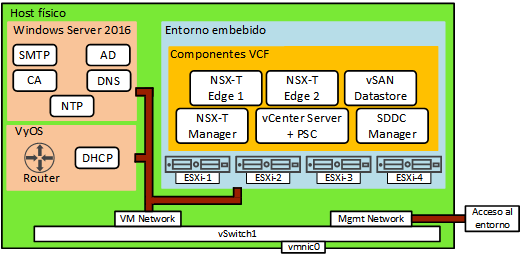
\includegraphics[width=0.6\textwidth]{imaxes/pruebaconcepto/hostFisico.png}
      \caption{Muestra la estructura generada por el instalador VLC. Cuatro hosts ESXi embebidos con los componentes de VMware Cloud Foundation cuyo tráfico circula a través del \textit{port group} VM Network.}
      \label{fig:estructura-generada-por-VLC}
    \end{figure}
    \begin{figure}[h]
      \centering
      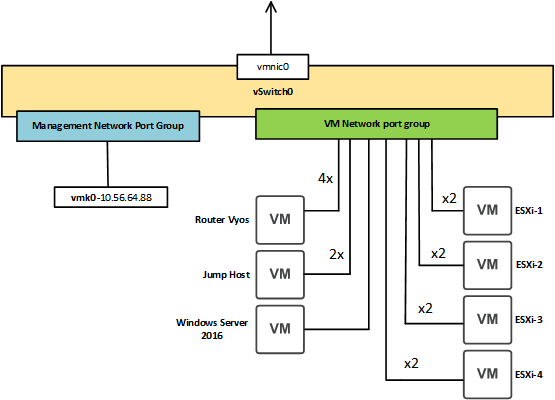
\includegraphics[width=0.6\textwidth]{imaxes/pruebaconcepto/vSwitch0HostFisico.png}
      \caption{Muestra las VMs que están funcionando sobre el host físico y que representan los componentes de la infraestructura física de un SDDC real, junto con el número de interfaces que se utilizan en cada una. Cada host ESXi generado por VLC cuenta con dos interfaces de red. El router VyOS, Jump Host y Windows Server 2016 se configuran antes del despliegue de VMware Cloud Foundation con VLC y se comunican con el entorno generado por VLC a través del \textit{port group} VM Network. El \textit{port group} Management Network se utiliza para acceder a la configuración del host físico a través de la dirección que se indica. Se utiliza la interfaz vmnic0 del host como salida del tráfico generado por el vSwitch0.}
      \label{fig:VMs-alojadas-host-fisico}
    \end{figure}
    \begin{figure}[h]
      \centering
      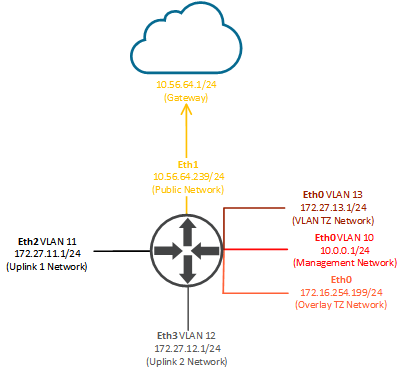
\includegraphics[width=0.4\textwidth]{imaxes/pruebaconcepto/RouterFisicoL3.png}
      \caption{Muestra la configuración del router VyOS. Cada una de las interfaces se debe configurar antes del despliegue de VCF. Todas usan MTU de 8940 Bytes. 
      En las interfaces Eth2 y Eth3 el router utiliza enrutamiento dinámico BGP donde el AS local es 65001 y el AS remoto es AS 65003, configurado para anunciar a sus vecinos la red 10.0.0.0/24 Management Network. Las direcciones configuradas como \textit{neighbour} son: 172.27.11.2, 172.27.11.3, 172.27.12.2 y 172.27.12.3. En la dirección IP 172.27.254.199 de la interfaz eth0, el router proporciona un servidor DHCP que asigna direcciones IP en el rango 172.16.254.0 - 172.16.254.100.}
      \label{fig:interfaces-router-fisico-L3}
    \end{figure}
    \begin{figure}[h]
      \centering
      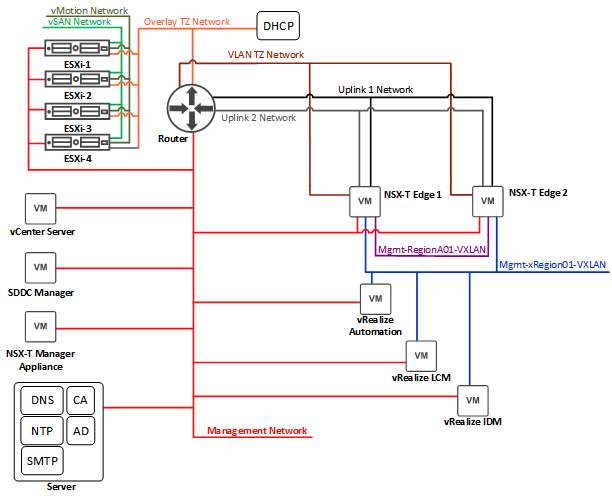
\includegraphics[width=0.6\textwidth]{imaxes/pruebaconcepto/RedDesdeDentro.png}
      \caption{Muestra todos los componentes de VMware Cloud Foundation desplegados por VLC, como se conectan con los distintos servicios de red y a que redes se conectan. Las redes Mgmt-xRegion01-VXLAN y Mgmt-Region01A-VXLAN se corresponden a redes virtuales gestionadas por VMware NSX-T que no requieren ninguna configuración adicional en la capa 3 de la infraestructura física (esto se verá con detalle en el apartado de diseño de VMWare NSX-T).}
      \label{fig:red-L3-infraestructura-fisica}
    \end{figure}
    \FloatBarrier
  \end{subsubsection}
  
\end{subsection}
    %%%%%DISEÑO ARQ. VIRTUAL
\begin{subsection}{Diseño y configuración del Management Domain}
    
    % Esta capa virtual provee infraestructura de almacenamiento, red y cómputo definida por software a través de servicios. En el modelo de despliegue consolidado de VMware Cloud Foundation, todos sus servicios y componentes se encuentran dentro de un mismo cluster (solo una AZ) dentro de la infraestructura, mientras que en el modelo estándar los servicios y componentes de gestión de la infraestructura están situados en clusters distintos (pueden estar en AZ distintas), todos sus componentes se encuentran agrupados en un mismo cluster.
    
    
    
    \subsubsection{Diseño de VMware vCenter Server}
    El componente VMware vCenter Server es el punto de acceso y de control de todas las máquinas virtuales localizados en los hosts ESXi que forman parte de su dominio. En el entorno desplegado se utiliza una instancia de VMware vCenter Server para controlar el \textit{management domain}, se denomina \textit{vcenter-mgmt}. Esta instancia de vCenter Server contiene un dominio que con un cluster vSphere formado por los cuatro hosts ESXi desplegados por VLC, estos se denominan respectivamente \textit{esxi-1}, \textit{esxi-2}, \textit{esxi-3} y \textit{esxi-4}. En vCenter Server se gestionan los recursos de las VMs de cada componente, se monitorizan los recursos, permite la creación y asignación de roles, permisos y usuarios, aisla las redes que usan los recursos que controla de otras instancias de vCenter Server, permite gestionar los grupos de discos de almacenamiento de cada host ESXi que forman el \textit{datastore} de VMware vSAN, administrar las redes a las que se conecta cada componente, en definitiva, VMware vCenter Server es el punto desde el cual se controlan los recursos que utiliza cada componente. Además, incluye el componente PSC que controla el dominio de autenticación de VMware vSphere SSO Domain denominado \textit{local}. Desde vCenter Server también se controlan las características de alta disponibilidad y recuperación ante fallos de VMware vSphere como se verá a continuación. El acceso a vCenter Server se hace a través del componente web vSphere Client.
    \begin{figure}[h]
      \centering
      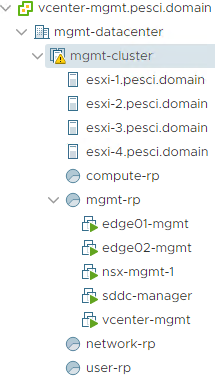
\includegraphics[width=0.2\textwidth]{imaxes/pruebaconcepto/clusterVCenterServer.png}
      \caption{Muestra el dominio (\textit{vcenter-mgmt.pesci.domain} de la instancia de vCenter Server y el cluster vSphere (\textit{mgmt-cluster}) donde se alojan los componentes del \textit{management domain}. Incluye cuatro hosts ESXi y cuatro \textit{resource pools}, uno de ellos contiene las VMs de los componentes dedicados a este \textit{management domain}.}
      \label{fig:cluster-vCenter-Server}
    \end{figure}
    \FloatBarrier
    %  Con vCenter Server se simplifica la escalabilidad del SDDC, la gestión de actualizaciones para los componentes es más sencilla, permite determinar roles específicos y responsabilidades y permite aislar las redes de otras instancias de vCenter Server. Además, para gestionar vSpehere SSO Domain, VMware vCenter Server contiene embebido el componente PSC con todos los servicios necesarios. 
    %  En caso de que existan varios \textit{Workload Domain} se puede habilitar el modo \textit{Enhanced Linked Mode} para poder gestionar todas las instancias de vCenter Server de forma centralizada desde un único vSphere Client.
    % Por lo anterior, en el \textit{management domain} se despliega una instancia de VMware vCenter Server que incluye un cluster de VMware vSphere.
    
    \begin{subsubsection}{Diseño almacenamiento VMware vSAN}
      El almacenamiento del \textit{management domain} desplegado, está implementado con VMwware vSAN. Los cuatro hosts ESXi contienen cuatro grupos de discos cada uno con configuración All-Flash. Como hay cuatro hosts participantes, soporta el fallo de un host lo cual permite dejar hosts fuera de servicio para tareas de mantenimiento. Esto es posible gracias a que con FTT (\textit{Failures-To-Tolerate}) igual a 1 se mantiene la redundancia de los datos almacenados en el \textit{datasotore}, en uno de los hosts. Cada grupo de discos cuenta con cuatro discos uno de ellos para caché, 16 discos en total. Para hacer disponible este servicio de almacenamiento, todos los hosts deben estar conectados a la subred generada para VMware vSAN y utilizar una VLAN para separar su tráfico.
    \end{subsubsection}
        
    \begin{subsubsection}{Diseño cluster VMware vSphere}
    Dentro de un \textit{workload domain} pueden existir varios clusters vSphere con diferentes características según su finalidad. Los hosts ESXi que lo forman pueden ser de diferentes tamaños teniendo en cuenta que se pueden usar menos hosts ESXi de mayor capacidad o más hosts con menores prestaciones, el coste de cada host ESXi, el uso que se le va a dar al cluster y las características máximas y mínimas del cluster vSphere. Para el \textit{management domain} se utiliza un único cluster vSphere con de 4 hosts de los cuales se reserva un host para proveer redundancia. Todos los hosts ESXi cuenta con 64GB de memoria RAM menos uno que tiene 32 GB, y 19.9GHz de CPU. Dentro del cluster hay que configurar los servicios vSphere HA y vSphere DRS para proteger los componentes del SDDC. La configuración que se establece en el \textit{management domain} es la siguiente:
    % En caso de que el \textit{management domain} esté extendido en dos AZ entonces se requieren 4 hosts en cada AZ para proporcionar redundancia y disponibilidad en caso de caída de una de las AZ.
   
    \begin{itemize}
        \item \textbf{vSphere High Availability}: en este servicio la propiedad \textit{Admission Control Policy} permite establecer la cantidad recursos reservados en caso de fallo y como se establece el cálculo de esos recursos. En el \textit{management domain} se configura para el fallo de al menos un host y reserva de recursos según un porcentaje, reservando así el 25\% de la CPU y el 30\% de la memoria RAM ya que funciona mejor cuando las VM usan mucha CPU y memoria. La otra propiedad que se debe habilitar para el correcto funcionamiento del servicio es \textit{VM and Application Monitoring}, que se encarga de reiniciar las VM en caso de caída.
        % que puede ser según el número hosts que pueden fallar en el cluster, según un porcentaje de reserva de rescursos o especificando el host donde se recolocan las VM del host caído.  RAM.  
        \item \textbf{vSphere DRS}: este servicio permite migrar VMs de un host ESXi a otro dentro del mismo cluster vSphere para equilibrar la carga de trabajo y mantener las VMs activas en caso de caída de alguno de los hosts. se activa usando la opción por defecto \textit{Fully Automated} ya que aporta el mejor balance entre consumo de recursos y migraciones de VM innecesarias. Adicionalmente se pueden establecer reglas para determinar reglas de orden de encendido sobre grupos de VM. 
        %En caso de que exista más de una AZ, se deben crear grupos de VM y de hosts de cada AZ para luego implementar reglas de afinidad para que las VM de una AZ no sean migradas a otra AZ ya que esto puede afectar al rendimiento de la VM. 
    \end{itemize}
    % En el modelo consolidado se debe crear un único cluster con un mínimo de cuatro hosts ESXi ya que uno de los hosts se utiliza para asegurar la disponibilidad del almacenamiento vSAN cuando hay algún host inactivo. Este modelo proporciona capacidad de un único fallo por cluster.
    \end{subsubsection}
    \subsubsection{Diseño de red para el cluster vSphere}
    Si bien en VMware Cloud Foundation existe VMware NSX-T, un componente dedicado únicamente a la administración de la red del SDDC, es desde VMware vSphere dónde se encuentran los elementos para establecer redes que separen cada tipo de tráfico de los componentes del SDDC. Estas redes se configuran en base a los siguientes aspectos:
    \begin{itemize}
        \item Separar el tráfico de cada servicio para mejorar la eficiencia de la red y la seguridad. Así se puede ajustar las características de cada red, como el ancho de banda o la latencia, a las necesidades de cada servicio.
        \item Utilizar un único vSphere Distributed Switch por cluster donde se añade un \textit{port groups} por cada servicio.
        % \item Mejorar el rendimiento usando NICs de tipo VMXNET3 en las máquinas virtuales.
        \item Las NICs físicas de cada host ESXi conectados a un mismo vSphere Distributed Switch están conectadas también a la misma red física.
        % \item Aquellas redes que se dedican a servicios de la infraestructura deben estar configuradas con puertos tipo \textit{vmkernel}.
    \end{itemize}
    Para el \textit{management domain} del SDDC se crea un único vSphere Distributed Switch llamado \textit{sddc-vds01} con la siguiente configuración:
    \begin{itemize}
        
        \item Se establece un MTU igual 9000 Bytes para permitir el tráfico de \textit{jumbo frames} ya que son requeridos por algunos de los servicios.
        
        \item Se habilita el servicio \textit{Network I/O} que permite establecer un nivel de prioridad a cada tipo de tráfico. Esto se realiza estableciendo limites de ancho de banda, políticas de balanceo de carga y reserva de recursos para un tipo de tráfico asociado a un servicio. Por cada tipo de tráfico hay cuatro aspectos que se pueden configurar que son \textit{Shares} (indica el \% de ancho de banda que se le da a un tipo de tráfico, el tipo de tráfico que tenga un mayor valor en \textit{Shares} tendrá más prioridad a la hora de usar los recursos), \textit{Reservation} (indica el valor de ancho de banda que se reserva para el tipo de tráfico) y \textit{Limit} (establece un valor máximo para el ancho de banda de un tipo de tráfico). En el \textit{management domain} los tipos de tráfico más relevantes que se deben configurar son los siguientes:
        \begin{itemize}
          \item \textit{Management Traffic}: el valor \textit{Shares} se establece al 50\% (\textit{Normal}) lo cual le da mayor prioridad que el resto de tipos. El resto de valores no se modifican.
          \item \textit{vSphere vMotion Traffic}: el valor \textit{Shares} se establece al 25\% (\textit{Low}) ya que durante el estado normal del entorno este tipo de tráfico no es muy importante. El resto de valores no se modifican.
          \item \textit{vSAN Traffic}: el valor \textit{Shares} se establece al 100\% (\textit{High}) para garantizar que este servicio recibe la cantidad de ancho de banda que necesita. El resto de valores no se modifican.
          \item \textit{Virtual Machine Traffic}: el valor \textit{Shares} se establece al 100\% (\textit{High}) para garantizar que las VMs siempre tienen acceso a la red ya que son una parte importante del SDDC. El resto de valores no se modifican.
        \end{itemize}
        
        \item Para detectar errores de compatibilidad entre la configuración del vSphere Distributed Switch y la red física se habilita el servicio \textit{Health Check}. Este se encarga de comprobar si la configuración de cada VLAN y MTU se adapta a la configuración de la capa física.
        
        \item Como puertos de salida \textit{Uplink} se configuran las interfaces físicas \textit{vmnic0} y \textit{vmnic1}. Como vDS es un componente distribuído, en cada host se usarán ambas interfaces de red como \textit{uplinks}.
        
    \end{itemize}
    En este vSpehere Distributed Switch para el \textit{management domain} se configuran los siguientes \textit{port groups}, que son de tipo \textit{Distributed port group} y de tipo \textit{Uplink port group}:
    \begin{itemize}
           
            \item \textbf{Management port group}: es un \textit{Distributed port group} que comunica a todos los hosts ESXi entre si y transmite el tráfico entre los diferentes componentes de VMware Cloud Foundation, es decir, por este \textit{port group} circulan los comandos de configuración y gestión que los componentes del SDDC se envían entre ellos. Con el nombre \textit{sddc-vds01-mgmt}, en él están configurados los cuatro hosts ESXi y las VMs \textit{vcenter-mgmt}, \textit{sddc-manager}, \textit{nsx-mgmt-1},\textit{edge01-mgmt} y \textit{edge02-mgmt} bajo la subred con IP 10.0.0.0, con máscara de red 255.255.255.0, con VLAN 10 y con MTU igual a 1500 Bytes. Esta red debe ser configurada también en la infraestructura física.
            
            \item \textbf{vMotion port group}: es un \textit{Distributed port group} que está dedicado al tráfico del componente vSphere vMotion para realizar las migraciones de máquinas virtuales de un host a otro. Con el nombre \textit{sddc-vds01-vmotion}, en él están configurados los 4 hosts bajo la subred con IP 10.0.4.0, con máscara de red 255.255.255.0, con VLAN 10 y con MTU igual a 8940 Bytes.
            
            \item \textbf{vSAN port group}: es un \textit{Distributed port group} que está dedicado al servicio de almacenamiento VMware vSAN y por él los hosts acceden al almacenamiento del SDDC. Con el nombre \textit{sddc-vds01-vsan}, en él están configurados los 4 hosts bajo la subred con IP 10.0.8.0, con máscara de red 255.255.255.0, con VLAN 10 y con MTU igual a 8940 Bytes.
            
            \item \textbf{Edge Uplink port group}: es un \textit{Distributed port group} dedicado a las conexiones del component NSX-T Edge que se dedica a dar acceso a determinados servicios y para proporcionar a otros \textit{workload domain} conexión con la red externa. Están gestionados por VMware NSX-T ya que dan servicio a sus componentes. En el entorno existen dos \textit{port groups} para proporcionar redundancia y alta dispobilidad, uno llamado \textit{sddc-edge-uplink01} cuyas instancias están configuradas bajo la red con IP 172.27.11.0 y con máscara de red 255.255.255.0, y otro llamado \textit{sddc-edge-uplink02} cuyas instancias están configuradas bajo la red con IP 172.27.12.0 y máscara de red 255.255.255.0. Ambos \textit{port groups} están configurados como VLAN Trunk (por ellos puede circular tráfico de cualquier VLAN) y tienen un MTU de 8940 Bytes. En los dos están configuradas dos VM llamadas \textit{edge01-mgmt} y \textit{edge02-mgmt}. Estas dos redes también se deben configurar en la infraestructura física.
            
            \item \textbf{Uplink port group}: se trata de un \textit{Uplink port group} al que se le asignan las NICs físicas de cada host para establecer políticas sobre el tráfico que se dirige desde los hosts y VMs hacia fuera del vSphere Distributed Switch. Con el nombre \textit{sddc-vds01-DVUplinks-10}, en él están configuradas las dos NICs físicas de cada host, cada una en una interfaz \textit{uplink}.
            
    \end{itemize}
    \begin{figure}[h]
      \centering
      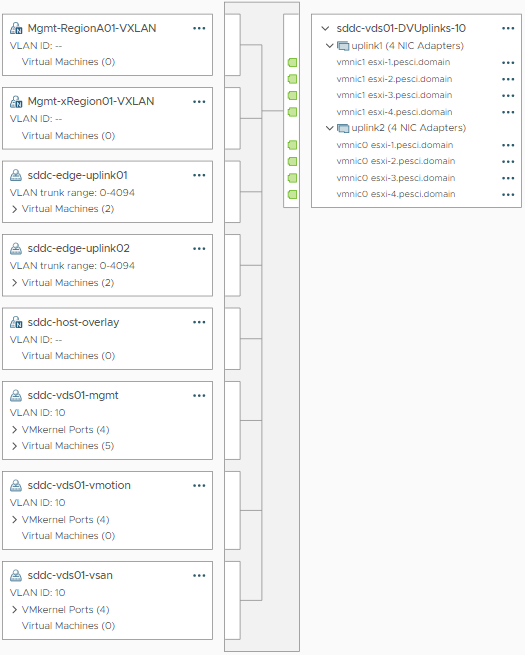
\includegraphics[width=0.4\textwidth]{imaxes/pruebaconcepto/distributedSwitchEntornoFinal.png}
      \caption{Muestra todos los \textit{Distributed Port Groups} y \textit{Uplink port group} que se alojan en el vSphere Distributed Switch (\textit{sddc-vds01}) dedicado al \textit{management domain}. En el \textit{port group} \textit{sddc-vds01-DVUplinks-10} se muestra como a cada interfaz \textit{uplink} se mapea una interfaz física (vmnic) de cada host ESXi. Los \textit{port groups} \textit{mgmt-Region01A-VXLAN}, \textit{mgmt-xRegion01-VXLAN} y \textit{sddc-host-overlay} son generados y administrados por el componente VMware NSX-T como se explicará más adelante. Cada \textit{port group} informa de cuantas VMs y hosts ESXi tiene conectados.}
      \label{fig:port-groups-vSwitch-vSphere}
    \end{figure}
    \FloatBarrier
    La configuración que se aplica a cada \textit{Distributed port group} descrito anteriormente es la siguiente:
    \begin{itemize}
      \item \textit{Port binding}: permite indidcar como se gestionan los puertos de un \textit{port group} cuando se añade o elimina una VM. Tiene dos opciones de configuración, la primera se denomina \textit{Static Port Binding} y su función consiste en asignar un puerto dentro del \textit{port group} a la VM que se conecta y solo se elimina cuando la VM es borrada. La segunda opción se denomina \textit{Ephemeral Port Binding} y consiste en que el puerto se asigna a la VM cuando esta se enciende y se elimina cuando se apaga o elimina. Para los \textit{port groups} \textit{sddc-vds01-vsan} y \textit{sddc-vds01-vmotion} se configura la opción \textit{Static Port Binding} ya que así se asegura que las VMs se conectan siempre al mismo puerto lo cual permite mantener datos históricos y hacer monitoreo a nivel de puerto. Para los \textit{port group} \textit{sddc-vds01-mgmt}, \textit{sddc-edge-uplink01} y \textit{sddc-edge-uplink02} se configura la opción \textit{Ephemeral Port Binding} ya que como el tráfico que circula por ellos es el que gestiona todos los componentes y da acceso a otras redes etonces se elimina la dependencia del estado de vCenter Server permitiendo que la comunicación continúe aunque vCenter Server no se encuentre operativo.
    
      \item \textit{Load Balancing}: indica como se distribuye el tráfico de salida de cada VM/host que se encuentran en el \textit{port group} entre las NICs físicas. Se selecciona \textit{Route based on physical NIC load}, es decir, el tráfico de una VM se transmite por una única NIC por lo que si esa NIC física está saturada, se asignará otra NIC física a la VM.
      
      \item \textit{Network failure detection}: esta opción permite establecer como debe determinar el \textit{port group} que alguna de las NICs físicas está fuera de servicio. Se selecciona \textit{Link status only} para que esto se determine según el estado que le transmite la NIC física, así se pueden detectar los fallos que ocurren en la red física.
      
      \item \textit{Notify switches}: se habilita para permitir a los host enviar \textit{frames} a los switches físicos para que estos conozcan la localización de las VM que están funcionando en cada host.
      
      \item \textit{Failback}: permite determinar como se reactiva una NIC cuando esta se recupera de un fallo. Se habilita para establecer que la NIC se marcará como activa inmediatamente después de que se haya recuperado. Esta opción se debería desactivar en caso de que el estado de la NIC sea inestable.
      
      \item \textit{Failover Order}: permite determinar que uplinks se deben utilizar, los que se seleccionan como \textit{active} son los que se utilizarán por defecto, los que se seleccionan como \textit{stand by} se usarán cuando los uplinks marcados como \textit{active} se encuentren desactivados. Se seleccionan las dos interfaces \textit{uplink} disponibles en el estado \textit{active}. Para el \textit{port group} \textit{sddc-edge-uplink01} se selecciona la interfaz \textit{uplink1} como activa y se deja sin usar la interfaz \textit{uplink2}, mientras que se configura de forma contraria en el \textit{port group} \textit{sddc-edge-uplink02}.
    \end{itemize}
    
    
    %%%%%%%%%%%%%%%%%%%%%%%%%%%%%%%%%%%%%%%%%%%%
    \subsubsection{Diseño de la red del SDDC con VMware NSX-T}
    En un SDDC debe existir una red virtual, es decir, definida por software o también conocida como \textit{Software-Defined Network}. Esta red al estar construída con componentes de software, se desacopla de la red física sobre la que funciona lo que hace posible que se pueda modificar sin necesidad de cambiar la configuración en la capa física, reduciendo así la complejidad de la red física y el tiempo dedicado a la gestión de la misma. Además, este tipo de arquitectura habilita la posibilidad de implementar múltiples configuraciones de red en tiempo reducido proporcionando elasticidad y flexibilidad a la hora de administrar los recursos, tanto para el administrador como para el usuario final.
    El componente encargado de crear, configurar y administrar la red virtualizada del SDDC es VMware NSX-T que a su vez contiene otros componentes entre los que se dividen distintas responsabilidades y funciones, ya descritos anteriormente.
    
    %%%%% 1 - EXPLICACION DE LOS COMPONENTES DE NSX Y LOS QUE HAY EN EL ENTORNO
    %%%%% 2 - COMO SE DEBE CONFIGURAR LA CAPA FÍSICA Y COMO ESTÁ IMPLEMENTADA EN EL ENTORNO ( parte de esto ya está definido en la parte de red física, REVISAR) => Meter la descripción de lo físico con el resto (modificar ese apartado) [https://docs.vmware.com/en/VMware-Validated-Design/6.0/sddc-architecture-and-design-for-the-management-domain/GUID-C924E896-D9C4-47BF-91D5-DF72605EF63E.html]
    %%%%% 3 - REDES QUE HAY Y COMO SE EXTIENDEN ENTRE AZs
    %%%%% 4 - COMO FUNCIONAN LAS COMUNICACIONES (GENEVE, ROUTING ...)
    
    % En esta sección se describe como VMware Cloud Foundation abstrae la red física en un conjunto de recursos virtuales de red, utilizando los servicios de VMware NSX para crear una capa virtual independiente de la infraestructura física.
    Aunque se recomienda desplegar tres instancias de NSX-T Manager en el \textit{management domain}, VLC solo despliega una única instancia llamada \textit{nsx-mgmt-1} para mejorar el rendimiento del entorno. Además, VLC también genera dos instancias de NSX-T Edge que se denominan \textit{edge01-mgmt} y \textit{edge02-mgmt}. %cada conjunto de instancias de cada componente forman un cluster donde cada VM está protegida por las funcionalidades vSphere HA y vSphere DRS para proveer alta disponibilidad del servicio y migrar las VMs a otra ubicación en caso de caída de una AZ o de un host. 
    Estas VMs están conectadas al \textit{port group} \textit{sddc-vds01-mgmt} que les permite comunicarse entre ellas y con vCenter Server, además las instancias de NSX-T Edge también están conectadas a otros dos \textit{Distributed port group} llamados \textit{sddc-edge-uplink01} y \textit{sddc-edge-uplink02}. %Si existe más de una AZ, varios de los \textit{distributed port groups} se deben extender al resto de AZs para que en caso de que la primera AZ falle sus VMs se puedan migrar a otra AZ y sigan teniendo conectividad. Los \textit{port groups} que deberían estar extendidos en todas las AZ son el \textit{port group} \textit{sddc-vds01-mgmt} de cada AZ\footnote{Cada AZ tiene su propio \textit{Management port group}, entonces en cada AZ debe ser accesible el \textit{Management port group} del resto de AZs.}, los \textit{port group} \textit{sddc-edge-uplink01}, \textit{sddc-edge-uplink02} y \textit{port group} \textit{Edge Overlay}.
    
    Los elementos que utiliza VMware NSX-T para crear una red independiente de la configuración de la red física son \textit{Segment} y \textit{Transport Zone}. Con estos componentes VMware NSX-T puede crear túneles que definen redes de capa 2 sin necesidad de realizar ningún cambio en la configuración de la red física.
    \begin{itemize}
      \item \textbf{Transport Zone} (TZ): define el alcance de la red virtual. Pueden ser de dos tipos distintos, basada en VLAN o basada en Overlay. Una TZ se puede asignar a varios TN que tendrán acceso a los \textit{segments} que funcionen en esa TZ. Un TN se conecta a una TZ a través de un N-VDS los cuales pueden pueden estar conectados a varias TZ de tipo VLAN pero solo a una TZ de tipo Overlay al mismo tiempo.
      
      \item \textbf{Segment}: también llamado \textit{Logical Switch}, representa un dominio de broadcast de capa 2 que forma parte de una \textit{Transport Zone}. El tipo de tráfico puede ser VLAN u Overlay dependiendo de como se haya configurado la \textit{Transport Zone} de la que forma parte. Las VMs de cada TN se pueden conectar a los \textit{Segments} situados en las \textit{Transport Zones} a las que el host está conectado. Estas VMs se pueden comunicar con el resto de VMs conectadas al mismo \textit{Segment}.
       
    \end{itemize}
    Para gestionar las conexiones de cada TN, tanto para los nodos NSX-T Edge como para los hosts ESXi, VMware NSX-T introduce el componente llamado \textbf{NSX-T Virtual Distributed Switch} (N-VDS). Cada TN del \textit{management domain} posee un N-VDS, este elemento conecta sus interfaces a los \textit{segments} que se configuran en cada TN. Para el \textit{management domain} del entorno, VLC despliega dos \textit{transport zones} diferentes.
    \begin{figure}[h]
      \centering
      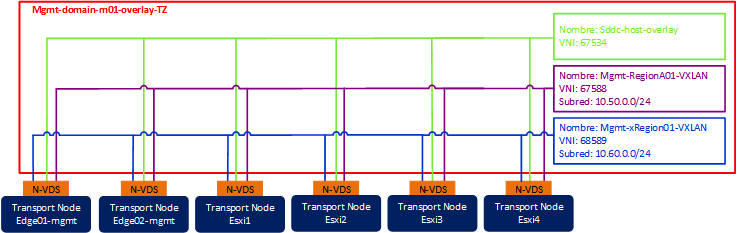
\includegraphics[width=1\textwidth]{imaxes/pruebaconcepto/OverlayTZSegments.png}
      \caption{Se muestra la \textit{transport zone} con el nombre \textit{mgmt-domain-m01-overlay-tz} de tipo Overlay. Está extendida en los seis TNs que hay en el \textit{management domain} y contiene tres \textit{segments}. El \textit{segment} \textit{mgmt-xRegion01-VXLAN} se utiliza para desplegar aplicaciones que deben ser accesibles desde todas las \textit{regions} que existan en el SDDC, es decir, la misma instancia de una aplicación está disponible desde varios puntos, así se reduce el consumo de recursos y aumenta la disponibilidad de esas aplicaciones ya que pueden migrar a distintas localizaciones según el estado de los recursos. El \textit{segment} \textit{mgmt-Region01A-VXLAN} tiene como finalidad alojar aplicaciones solo deben ser accesibles desde dentro de una misma \textit{region}. En estos dos \textit{segments} es donde se colocan los productos de VMware vRealize. Por último, el \textit{segment} \textit{sddc-host-overlay} es utilizado por los componentes de VMware NSX-T para comunicarse con y entre los diferentes TNs. VMware NSX-T genera en el vSphere vSwitch un \textit{port group} por cada \textit{segment} para poder conectar la VM de cada componente al \textit{port group} que le corresponda.}
      \label{fig:overlay-TZ-segments-NSXT}
    \end{figure}

    \begin{figure}[h]
      \centering
      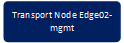
\includegraphics[width=1\textwidth]{imaxes/pruebaconcepto/VLANTZSegments.png}
       \caption{Muestra la\textit{transport zone} con el nombre \textit{sfo01-m01-edge-uplink-tz} de tipo VLAN. Está extendida en los dos TNs \textit{edge01-mgmt} y \textit{edge02-mgmt} y contiene dos \textit{segments}. Ambos \textit{segments} \textit{VCF-edge-mgmt-cluster-segment-11} y \textit{VCF-edge-mgmt-cluster-segment-12} son utilizados por las instancias de NSX-T Edge para transmitir el tráfico que proviene de los \textit{segments} donde se despliegan aplicaciones hacia la red externa (esto se explicará con más detalle). Estos \textit{segments} utilizan los \textit{port groups} \textit{trunk} del vSphere Switch para transmitir su tráfico hacia las interfaces de red físicas de cada host.}
      \label{fig:VLAN-TZ-segments-NSXT}
    \end{figure}

    \FloatBarrier
    %\begin{itemize}
      % \item \textit{mgmt-domain-m01-overlay-tz}:
      %   \begin{itemize}
      %     \item Tipo: Overlay
      %     \item Transport Nodes: \textit{edge01-mgmt}, \textit{edge02-mgmt}, \textit{esxi1}, \textit{esxi2}, \textit{esxi3} y \textit{esxi4}.
      %     \item Segments:
      %       \begin{itemize}
      %         \item \textit{mgmt-xRegion01-VXLAN}:
      %           \begin{itemize}
      %             \item VNI: 68589
      %             \item Subred: 10.60.0.0/24
      %             \item VMs: \textit{vrlcm} (10.60.0.60), \textit{vridm} (10.60.0.30)
      %             \item Descripción: se usa para desplegar las aplicaciones (algunos productos de VMware vRealize Suite lo utilizan) que deben ser accesibles desde todas las \textit{Regions} del SDDC, por lo tanto este \textit{segment} debe estar extendido en todo el entorno para que las VMs que se alojen en él puedan mantener la misma configuración de red independientemente del lugar físico donde se encuentren.
      %           \end{itemize}
      %         \item \textit{mgmt-Region01A-VXLAN}:
      %           \begin{itemize}
      %             \item VNI: 67588
      %             \item Subred: 10.50.0.0/24
      %             \item Descripción: su finalidad es alojar aplicaciones que sean accesibles desde una misma \textit{Region}. El alcance de estas aplicaciones está limitado a una \textit{Region} por lo tanto este \textit{segment} solo está extendido dentro de la misma.
      %           \end{itemize}
      %         \item \textit{sddc-host-overlay}:
      %           \begin{itemize}
      %             \item VNI: 67534
      %             \item Descripción: \textit{segment} usado por los componentes de VMware NSX-T para comunicarse entre los diferentes hosts ESXi.
      %           \end{itemize}
      %       \end{itemize}
      %   \end{itemize}
    %   \item \textit{sfo01-m01-edge-uplink-tz}:
    %     \begin{itemize}
    %       \item Tipo: VLAN
    %       \item Transport Nodes: \textit{edge01-mgmt} y \textit{edge02-mgmt}.
    %       \item Segments:
    %         \begin{itemize}
              
    %           \item \textit{VCF-edge-mgmt-cluster-segment-11}:
    %             \begin{itemize}
    %               \item VLAN: 11
    %               \item VMs: \textit{edge01-mgmt} (172.27.11.2/24) y \textit{edge02-mgmt} (172.27.11.3/24).
    %               \item Descripción: usado para transmitir el tráfico saliente hacia la red física.
    %             \end{itemize}
    %           \item \textit{VCF-edge-mgmt-cluster-segment-12}:
    %             \begin{itemize}
    %               \item VLAN: 12
    %               \item VMs: \textit{edge01-mgmt} (172.27.12.2/24) y \textit{edge02-mgmt} (172.27.12.3/24).
    %               \item Descripción: usado para transmitir el tráfico saliente hacia la red física.
    %             \end{itemize}
    %         \end{itemize}
    %       \end{itemize}
    % \end{itemize}
    
    Las TZ, tanto las basadas en Overlay como las basadas en VLAN, sirven para comunicar TNs que se encuentran en distintas partes de la infraestructura física (por ejemplo, en distintos racks) como si estuvieran situadas en el mismo dominio broadcast de capa 2 físico. 
    Aquellas que usan Overlay utilizan el protocolo Geneve para crear un túnel entre los puntos de origen y destino por el cual circula el tráfico generado por los \textit{segments} que pertenecen a esa TZ y que debe salir a la red física para alcanzar su destino. El protocolo Geneve añade una cabecera UDP a cada paquete Ethernet que generan los \textit{segments} cuando este sale del TN donde se generó hacia un TN situado en otra red física. La nueva cabecera incorpora un identificador llamado VNI y es único para cada \textit{segment} (cada \textit{segment} tiene su propio identificador VNI). 
    \begin{figure}[h]
      \centering
      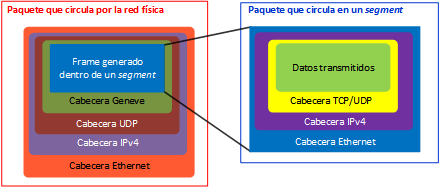
\includegraphics[width=1\textwidth]{imaxes/pruebaconcepto/FrameGeneve.png}
      \caption{Muestra las cabeceras que forman un paquete de red que pertenece a un \textit{segment} cuando este sale de un TN. Cuando el paquete que circula por la red virtual (contiene los datos que se transmiten y la información de las VMs origen y destino) tiene salir a la infraestructura física para alcanzar el destino, el \textit{transport node} añade la cabecera del protocolo Geneve con el identificador VNI correspondiente, una cabecera UDP con un puerto origen y destino establecidos por defecto, una cabecera IP con las direcciones IP origen y destino de los TN que se están comunicando, y una cabecera Ethernet donde se idican las direcciones MAC de los TN origen y destino. Así, dos VMs conectadas al mismo \textit{segment} pero alojadas en TNs de dominios broadcast diferentes, pueden comunicarse de forma transparente como si estuvieran conectadas directamente una con la otra en la misma subred.}
      \label{fig:Frame-Geneve-Segment-NSXT}
    \end{figure}
    \FloatBarrier
    % \begin{figure}[h]
    %   \centering
    %   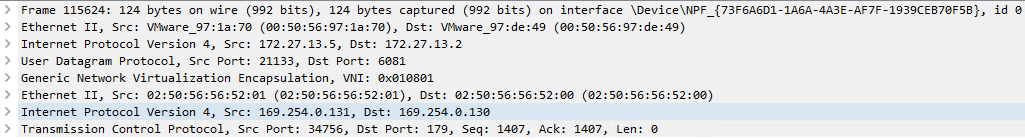
\includegraphics[width=1\textwidth]{imaxes/pruebaconcepto/FrameExampleGeneve.png}
    %   \caption{Cabeceras de un paquete capturado con el programa Wireshark que utiliza encapsulación Overlay. Contiene un VNI, las direcciones IP de los elementos que se comunican dentro del \textit{segment} y las direcciones IP de los TN que se comunican \textit{}}
    %   \label{fig:Frame-Geneve-Example-NSXT}
    % \end{figure}
    En las TZ de tipo VLAN, tráfico de sus \textit{segments} es encapsulado añadiendo un identificador de VLAN definido en una plantilla \textit{Uplink Policy}\footnote{A las TZ de tipo Overlay no se les aplica ninguna \textit{Uplink Policy}.} que se asigna a la TZ. Se aplica la misma VLAN para encapsular el tráfico de todos los \textit{segments} de una misma TZ de tipo VLAN. Estas plantillas permiten establecer como debe el N-VDS de un TN tratar el tráfico de la \textit{transport zone} a la que se asigna. En cada una se especifican varias \textit{Teaming Policy}, la VLAN que debe usar el N-VDS cuando tiene que enviar el tráfico fuera del TN y el MTU de cada interfaz \textit{uplinks}. Una \textit{Teaming Policy} indica como el N-VDS utiliza los \textit{uplinks} a nivel de \textit{segment} para distribuir el tráfico y conseguir conexiones redundantes y balanceo de la carga, se especifica una \textit{Teaming Policy} por defecto más otras adicionales. Se aplica una \textit{Uplink Policy} a la TZ de tipo VLAN  \textit{sfo01-m01-dge-uplink-tz}.
    %***UPLINKPOLICY**%
    %  Además, en una \textit{Uplink Policy} se define un mapeo con las interfaces \textit{uplink} establecidas en vSphere Distributed Switch (uplink1 y uplink2) para dirigir el tráfico de cada TZ hacia la red física. 
    %Los TNs \textit{edge01-mgmt} y \textit{edge02-mgmt} proporcionan acceso a la red externa a los \textit{segments} de VMware NSX-T, por ello requieren estar conctados a los dos tienen sus interfaces conectadas a los \textit{uplinks} están mapeados con las NICs físicas de cada host ESXi a través de  a los que están ancladas ambas VMs, es decir, un \textit{uplink} está mapeado con una NIC física del host ESXi. 
    %En las TZ de tipo VLAN, se utilizan plantillas .
    \begin{figure}[h]
      \centering
      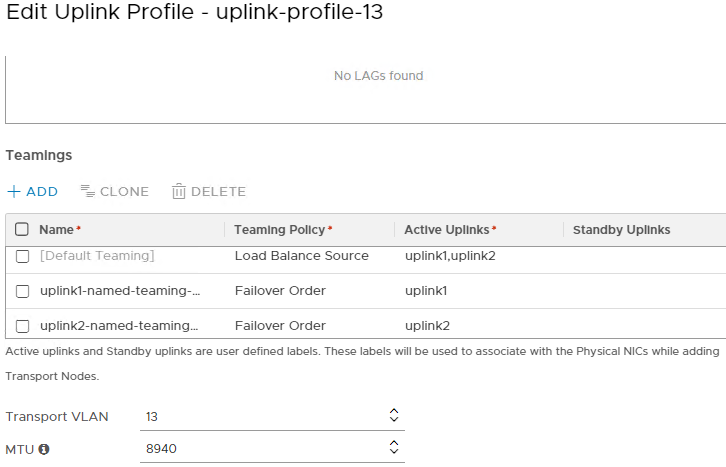
\includegraphics[width=1\textwidth]{imaxes/pruebaconcepto/UplinkPolicy13.png}
      \caption{Muestra la \textit{Uplink Policy} (\textit{uplink-profile-13}) configurada para la TZ \textit{sfo01-m01-dge-uplink-tz}. Se establece la VLAN 13 como Transport VLAN, utilizado para encapsular el tráfico saliente hacia la red física, y MTU de 8940 Bytes para los uplinks. Hay definidas tres \textit{Teaming Policies}, una por defecto (\textit{Default teaming}) que utiliza \textit{Load Balance Source} para hacer un mapeo uno a uno entre las interfaces de cada VM y uno de los \textit{uplinks} (todo el tráfico correspondiente a esa interfaz se envía y recibe por el mismo \textit{uplink}), y dos adicionales \textit{uplink1-named-teaming-policy} y \textit{uplink2-named-teaming-policy} que utilizan \textit{Failover Order} donde se establece un \textit{uplink} como activo por donde se transmite todo el tráfico y otros de reserva que se usan en caso de que el \textit{uplink} activo falle (en una de las políticas todo el tráfico se reenvía por \textit{uplink1} y en la otra por \textit{uplink2}).}
      \label{fig:Uplink-Policy-13-NSXT} 
    \end{figure}
    \FloatBarrier
    A los \textit{segments} \textit{VCF-edge-mgmt-cluster-segment-11} y \textit{VCF-edge-mgmt-cluster-segment-12} pertenecientes a la TZ \textit{sfo01-m01-dge-uplink-tz} se les asigna la \textit{Teaming Policy} \textit{uplink1-named-teaming-policy} y \textit{uplink2-named-teaming-policy} respectivamente. De esta forma se consigue que el tráfico que circula por cada uno de ellos solo utilice un único \textit{uplink}. 
    \begin{figure}[h]
      \centering
      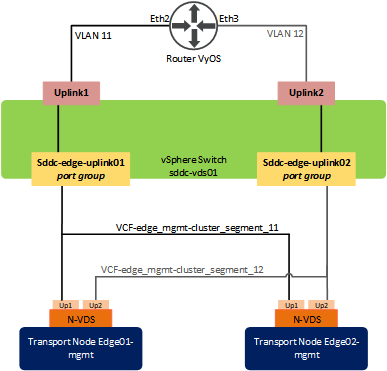
\includegraphics[width=0.6\textwidth]{imaxes/pruebaconcepto/UplinkDesign.png}
      \caption{Muestra la topología que forman las instancias de NSX-T Edge para generar la redundancia y alta disponibilidad en las rutas hacia la red externa para las aplicaciones cuya red está gestionada por VMware NSX-T, desde el punto de vista de VMware vSphere. Cada TN Edge posee dos interfaces \textit{uplink} que durante su configuración se mapea cada una con uno de los \textit{trunk port groups} de vSphere Switch. Las interfaces \textit{uplink} que se indican en la \textit{Teaming Policy} se refieren a las de la instancia de NSX-T Edge, no las de vSphere vSwitch, por lo tanto cada uno de los \textit{segments} utiliza solo uno de los \textit{uplinks} que combinado con la configuración de los \textit{port groups} de vSphere vSwitch establecen las rutas que se muestran en la imagen.}
      \label{fig:Uplink-Design-Edge-NSXT} 
    \end{figure}
    \FloatBarrier
    % Así, como cada TN de NSX-T Edge está anclado a dos \textit{trunk port groups} en vSphere Switch por donde se transmite el tráfico de estos dos \textit{segments} y cada uno de esos \textit{segments} transmite por un único \textit{uplink}, se consigue que estas rutas hacia la red externa sean redundantes y con alta disponibilidad para las aplicaciones cuya red está gestionada por VMware NSX-T.
    % Para la TZ de tipo VLAN \textit{sfo01-m01-dge-uplink-tz} se especifica la siguiente \textit{Uplink Policy}:
    % \begin{itemize}
    %   \item Nombre: \textit{uplink-profile-13}
    %   \item Transport VLAN: 13
    %   \item MTU: 8940
    %   \item Teaming Policy: se especifican tres, una por defecto y dos adicionales:
    %     \begin{itemize}
    %       \item \textit{Default teaming}: \textit{Load Balance Source}, hace un mapeo uno a uno entre cada interfaz virtual de cada VM y uno de los \textit{uplinks} del N-VDS, así todo el tráfico correspondiente a esa interfaz se envía y recibe por el mismo \textit{uplink}.
          
    %       \item \textit{uplink1-named-teaming-policy}: \textit{Failover Order}, se establece un \textit{uplink}, \textit{uplink1} en este caso, como activo que se utiliza para enviar todo el tráfico, y una lista de \textit{uplinks} ordenados que se utilizan en caso de que el primero no esté disponible, vacía para esta \textit{Teaming policy}.
    %       \item \textit{uplink2-named-teaming-policy}: \textit{Failover Order}, donde el \textit{uplink} activo es \textit{uplink2} y la lista de \textit{uplinks} de reserva está vacía.
    %     \end{itemize}
    % \end{itemize}
    % A los \textit{segments} de esta TZ, \textit{VCF-edge-mgmt-cluster-segment-11} y \textit{VCF-edge-mgmt-cluster-segment-12} se les asignan las \textit{Teaming Policy} \textit{uplink1-named-teaming-policy} y \textit{uplink2-named-teaming-policy} respectivamente. Con esta configuración el tráfico de cada \textit{segment} circula por una única NIC física del host ESXi. Esto, junto con la configuración \textit{Failover Order} establecida para los \textit{port groups} \textit{sddc-edge-uplink01} y \textit{sddc-edge-uplink02} en el vSphere vDS,se consigue que el tráfico de salida hacia la red física perteneciente a los componentes de VMware NSX-T y todas las aplicaciones cuya red gestiona VMware NSX-T, sea distribuído por dos redes distintas proporcionando redundancia y disponibilidad del servicio en caso de que ocurra una caída de alguna de las conexiones.
    %*****************%

    Esta encapsulación, tanto VLAN como Overlay, tiene lugar cuando los paquetes salen de la interfaz de una VM y entran en el N-VDS del TN. Para ello, cada TN tiene dispositivo llamado \textit{Tunnel End Point} (TEP) al que se le asigna una dirección IP utilizada para enviar y recibir el tráfico entre VMs que se encuentran en el mismo \textit{segment} pero se alojan en TNs situados en redes L2 diferentes\footnote{En el entorno desplegado todos los TN se encuentran dentro de la misma red física. Esto implica que no se genere tráfico con los TEPs ya que todas las TZs funcionan sobre un único dominio broadcast.}. Los TNs que son hosts ESXi obtienen su dirección TEP de un servidor DHCP\footnote{El servidor DHCP hace que se simplifique el proceso de configuración de un nuevo host ESXi ya que le asigna una dirección IP de forma automática.} mientras que los que son instancias de NSX-T Edge la dirección IP se asigna de forma manual. El TEP de cada TN tiene dos direcciones IP asignadas puesto que cada uno tiene dos interfaces de red, \textit{esxi-1} tiene las direcciones 172.16.254.10 y 172.16.254.11, \textit{esxi-2} tiene las direcciones 172.16.254.12 y 172.16.254.13, \textit{esxi-3} tiene las direcciones 172.16.254.14 y 172.16.254.15, \textit{esxi-4} tiene las direcciones 172.16.254.16 y 172.16.254.17, \textit{edge01-mgmt} tiene las direcciones 172.27.13.2 y 172.27.13.3, y \textit{edge02-mgmt} tiene las direcciones 172.27.13.4 y 172.27.13.5.
    
    Al crear un \textit{segment} dentro de una TZ, se configura un modo de replicación que indica como se retransmite el tráfico Broadcast, Multicast y Unknown Unicast propio del \textit{segment} cuando este tiene que viajar a un TN que está en una ubicación distinta en el medio físico. El modo de replicación que se utiliza en todos los \textit{segments} es \textit{Two-Tier Hierarchical Mode}. 
    \begin{figure}[h]
      \centering
      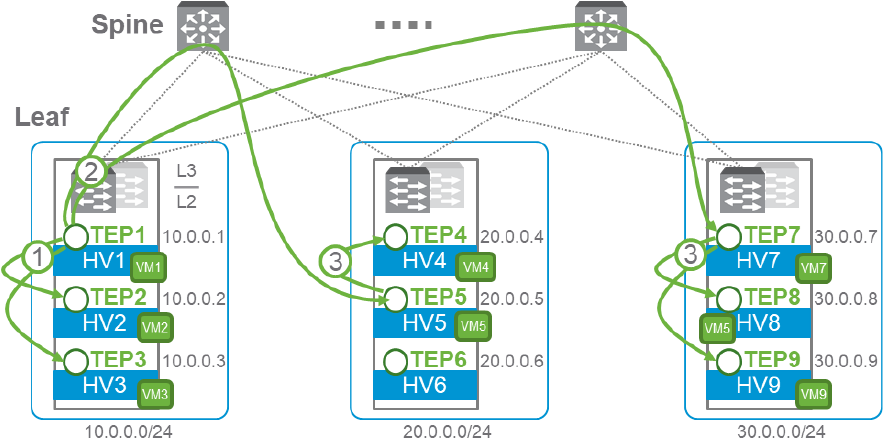
\includegraphics[width=0.6\textwidth]{imaxes/pruebaconcepto/Two-tier-ReplicationMode.png}
      \caption{Ejemplo de como funciona el modo de replicación \textit{Two-Tier Hierarchical}. (1) Cuando el TN HV1 envía tráfico BUM a la red primero lo hace a los TNs que están en su mismo dominio, (2) después envía una copia de ese tráfico a un único TN de cada dominio broadcast donde exista el \textit{segment} propietario del tráfico y, finalmente, (3) el TN de cada localización lo retransmite al resto de TNs de su dominio que lo requieran. De este modo se reduce el número de paquetes que el TN origen debe enviar a través de la red física.}
      \label{fig:Frame-Geneve-Segment-NSXT}
    \end{figure}
    \FloatBarrier
    % Este consiste en que cuando desde un TN se envía algún tipo de tráfico BUM de un \textit{segment} cuyos TNs están distribuídos en distintos puntos de la infraestructura física, el TEP del TN origen detecta que debe retransmitir el tráfico a una red externa, en la red externa se selecciona un TN que recibe el tráfico y lo reenvía al resto de TNs dentro del mismo dominio de red que deben recibir ese tráfico, así se reduce . El tráfico solo se enviará a los TN que contienen VMs que forman parte del \textit{segment} que lo genera. Es el componente NSX-T Controller quien se encarga de actualizar e indicar a los TNs toda la información para que esta comunicación sea correcta.
    
    El objetivo es crear nuevas subredes, es decir \textit{segments} que se expanden por los distintos TNs adheridos a la \textit{transport zone} correspondiente, y conectarlas a un router virtual para al final formar subredes distribuidas con servicios de red también	distribuidos y virtualizados, todo gestionado desde VMware NSX-T y sin tener que configurar la red física. Para completar esto, VMware NSX-T introduce routers virtuales que se encuentran embebidos y distribuídos dentro del hypervisor ESXi de cada TN y que proporcionan enrutamiento entre \textit{segments} y servicios de red distribuídos. Permiten definir un \textit{gateway} para cada \textit{segment} a través del cual las VMs conectadas pueden acceder a la red externa y los servicios de red. La herramienta VLC despliega para el \textit{management domain} un modelo de enrutamiento de doble capa (\textit{Two Tier Routing}) donde se utilizan dos routers virtuales, \textit{Tier-0} (\textit{mgmt-domain-tier0-gateway}) dedicado a gestionar el acceso a la red externa a través del router VyOS con conexiones redundantes, y \textit{Tier-1} (\textit{mgmt-domain-tier1-gateway})que gestiona el enrutamiento entre \textit{segments} y proporciona servicios de red a las VMs.

    \begin{figure}[h]
      \centering
      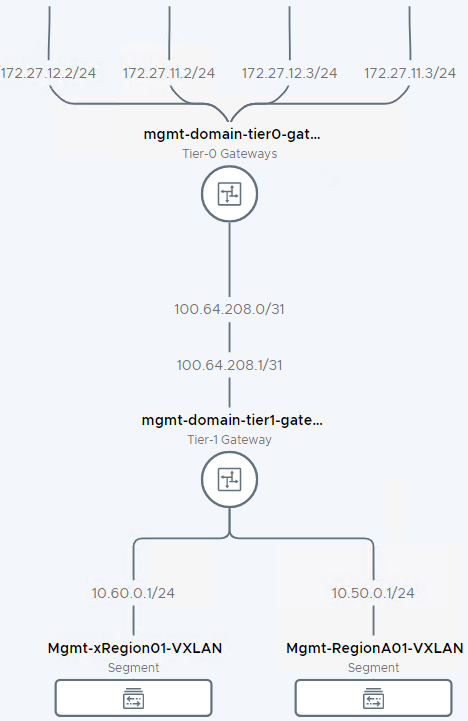
\includegraphics[width=0.5\textwidth]{imaxes/pruebaconcepto/topologiaTwoTierRouting.png}
      \caption{Muestra la topología del modelo de dos routers virtuales y los \textit{segments} a los que se conecta cada uno desde el punto de vista de NSX-T. El router de Tier-1 enruta el tráfico entre los \textit{segments} a los que está conectado y hacia el router de Tier-0 que se encarga de transmitir el tráfico hacia la red física.}
      \label{fig:Topology-TwoTier-Routing-NSXT}
    \end{figure}
    \FloatBarrier
    Un router router lógico está formado por dos componentes:
    \begin{itemize}
      
      \item \textbf{Distributed Router} (DR): que gestiona el enrutamiento y se a subredes a través de sus interfaces lógicas. Estas subredes pueden ser \textit{segments} u otro DR. A cada interfaz se le asigna una dirección MAC y una dirección IP que representa el \textit{gateway} de la subred. Este componente está distribuído en todos los TN, tanto hosts ESXi como instancias de NSX-T Edge manteniendo la misma configuración (interfaces,tablas de enrutamiento, etc.). Su función es redirigir el tráfico que recibe entre las interfaces que tiene disponibles, es decir, enruta el tráfico entre los diferentes \textit{segments} a los que está conectado el router virtual Tiene una interfaz llamada \textit{Internal transit Link} conectada a la red \textit{Internal Transit Network} que se utiliza para conectar todos los DR y SR de un \text{Tier} distribuídos en los TN.
      
      \item \textbf{Service Router} (SR): proporciona servicios de red de forma centralizada (NAT, DHCP, Load Balancer, VPN, Gateway Firewall y Bridging L2) y proporciona acceso a la red externa. Este componente no está distribuído entre los diferentes TN, solo se se encuentra distribuido en las instancias de NSX-T Edge. Los servicios que proporciona solo se entregan a los recursos cuya red está gestionada por VMware NSX-T. Posee la interfaz \text{Internal Transit Link} para comunicarse con el resto de DR y SR pertenecientes al mismo \text{Tier}, dos interfaces \textit{External Interface} que se conectan a los \text{segments} que dan acceso a la red externa \footnote{La \textit{External Interface} solo existe en \textit{Tier-0} ya que es el router que se comunica con el dispositivo físico.}, la interfaz \textit{Router Link}\footnote{Router Link Network utiliza por defecto la subred 100.64.0.0/16.} que conecta el SR de \textit{Tier-0} con el de \textit{Tier-1}, y la interfaz \textit{Internal transit} que se habilita cuando se activa la opción \textit{Inter SR iBGP}\footnote{Inter SR iBGP Network utiliza por defecto la subred 169.254.0.0/24.} y que comunica los SR de las dos instancias de NSX-T Edge.
    \end{itemize}

    \begin{figure}[h]
      \centering
      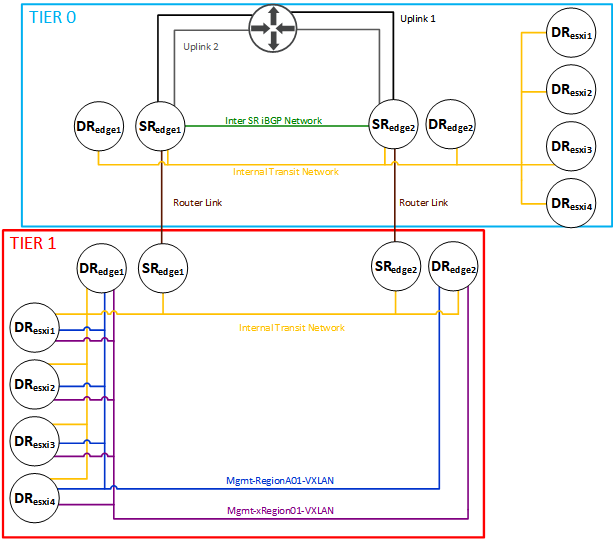
\includegraphics[width=0.8\textwidth]{imaxes/pruebaconcepto/EstructuraInternaTiers.png}
      \caption{Muestra los componentes internos de cada router virtual y como estos están distribuidos por todos los TNs. El router \textit{mgmt-domain-tier0-gateway} tiene el componente SR distribuído en dos TN que son las instancias de NSX-T Edge, y el componente DR distribuido en todos los TNs. El SR situado en \textit{edge01-mgmt} está conectado al \textit{segment} \textit{VCF-edge\_mgmt-edge-cluster-segment-11} y usa la dirección IP 172.27.11.2, y otra interfaz conectada al \textit{segment} \textit{VCF-edge\_mgmt-edge-cluster-segment-12} donde usa la IP 172.27.12.2, mientras que el SR de \textit{Tier-0} situado en \textit{edge02-mgmt} se conecta a los mismos \textit{segments} pero usando las direcciones 172.27.11.3 y 172.27.12.3 respectivamente. El router \textit{mgmt-domain-tier1-gateway} tiene el componente SR distribuido en las dos instancias de NSX-T Edge y el componente DR distribuido por en todos los TNs. Ambos SR están conectados con los SR de \textit{Tier-0} para transmitir el tráfico hacia la red física. Los DR de \textit{Tier-1} están conectados a los \textit{segments} \textit{Mgmt-RegionA01-VXLAN} y \textit{Mgmt-xRegion01-VXLAN} para proporcionar enrutamiento y servicios a las VMs situadas en ellos.}
      \label{fig:estructura-interna-TwoTier-Routing-NSXT}
    \end{figure}
    \FloatBarrier
    
    La razón de tener dos capas de enrutamiento se debe a la configuración del router \textit{mgmt-domain-tier0-gateway}. En este router se utiliza BGP para comunicarse con el router físico a través de las \textit{external interfaces} (se establece 65003 como \textit{autonomous system} local)\footnote{El uso de BGP simplifica la configuración de nuevas rutas cuando se añaden componentes al entorno, y que no se pierda la conectividad en caso de caída de alguna de las interfaces. Este protocolo también se configura en las interfaces del router Vyos}, la opción \textit{Inter SR iBGP} establecer una comunicación mediante BGP entre las instancias distribuídas del componente SR de \textit{Tier-0} para que se pueda seguir transmitiendo el tráfico en caso de que alguna de las interfaces de una instancia de NSX-T Edge esté fuera de servicio, se activa el protocolo ECMP para balancear el tráfico hacia la red física entre los caminos disponibles ya que en conjunto, en el router de \textit{Tier-0} existen cuatro rutas posibles para alcanzar el router VyOS. Un aspecto importante es la configuración de la disponibilidad de un router virtual ya que determina el modo en el que se va a ejecutar. En el router de \textit{Tier-0} se selecciona el modo \textit{active-active} el cual implica que las dos instancias de SR funcionan ambas de forma activa, es decir, el tráfico que reciba cada una será encaminado por una subred diferente proporcionando así mayor ancho de banda, mayor disponibilidad y mayor escalabilidad. Esto esto último no es compatible con servicios de red centralizados, por ello es necesario desplegar al menos un router lógico de \textit{Tier-1} (\textit{mgmt-domain-tier1-gateway}) configurado con el modo \textit{active-stanby} el cual solo se utiliza una de las dos instancias del SR de \textit{Tier-1} por lo tanto el tráfico dirigido a este router siempre será recogido en un único punto. Así, en el router \textit{mgmt-domain-tier1-gateway} es donde se pueden desplegar servicios de red como NAT, Load Blancing, DNS y VPN, para los \textit{segments} que están conectados.
    % Las interfaces de cada router lógico son de los siguientes tipos:
    
    % \begin{itemize}
    %   \item \textit{External Interface}: se refiere a las interfaces que conectan con el dispositivo de la red física, normalmente un router.
    %   \item \textit{Internal Transit Link}: está interfaz conecta a todos los DR de \textit{Tier-0} distribuídos en cada TN con los SR formando una única red.
    %   \item \textit{RouterLink Interface}: interfaz que conecta un router lógico de \textit{Tier-1} con uno de \textit{Tier-0} a través de una subred generada por defecto (100.64.0.0/16).
    % \end{itemize}
    
    % Los routers lógicos creados para el \textit{management domain} en el entorno tienen la siguiente configuración:
    
    % \begin{itemize}
    %   \item \textbf{mgmt-domain-tier0-gateway}: su función consiste en proporcionar acceso a la red física.
    %     \begin{itemize}
    %       \item \textit{External Interfaces}\footnote{Estas direcciones corresponden a las interfaces de los TN NSX-T Edge que conectan con las interfaces Uplink sobre dos \textit{segments} de tipo VLAN.}: Dos que se conectan al \textit{segment} \textit{VCF-edge\_mgmt-edge-cluster-segment-11} (172.27.11.2 y 172.27.11.3) y dos que se conectan al \textit{segment} \textit{VCF-edge\_mgmt-edge-cluster-segment-12} (172.27.12.2 y 172.27.12.3).
    %       \item \textit{Internal Transit Link}: Usa la subred 169.254.0.0/24.
    %       \item \textit{RouterLink Interface}: Tiene la dirección 100.64.192.0/31.
    %       \item Configuración: se 
    %       \item Configuración HA: determina el modo en el que se va a ejecutar el router de \textit{Tier-0}. En este caso se selecciona el modo \textit{active-active} el cual implica que las instancias de SR (una en cada nodo NSX-T Edge) funcionan ambas de forma activa, el tráfico que reciba cada una será encaminado por una subred diferente. Es por esto que el router lógico de \textit{Tier-0} no puede ofrecer servicios centralizados.
    %     \end{itemize}
    
    %   \item \textbf{mgmt-domain-tier1-gateway}: router de \textit{Tier-1} dedicado a gestionar el enrutamiento de las VMs de aplcaciones no dedicadas a la administración del SDDC. 
    %   \begin{itemize}
    %     \item \textit{Internal Transit Link}: Usa la subred 164.254.0.0/24.
    %     \item \textit{RouterLink Interface}: Tiene la dirección 100.64.192.1/31.
    %     \item \textit{Segment Interfaces}: conectado al \textit{segment} \textit{mgmt-Region01A-VXLAN} con la dirección IP 10.50.0.1, y al \textit{segment} \textit{mgmt-xRegion01-VXLAN} con la dirección IP 10.60.0.1.
    %     \item Configuración HA: determina el modo en el que se va a ejecutar el router de \textit{Tier-1}. En este caso se selecciona el modo \textit{active-stanby} el cual solo utiliza una de las dos instancias del SR de \textit{Tier-1} (cada una en un nodo de NSX-T Edge) por lo tanto el tráfico que reciba solo será encaminado por un único punto. Esto permite activar servicios centralizados, por lo tanto será \textit{mgmt-domain-tier1-gateway} y no \textit{mgmt-domain-tier0-gateway} el encargado de proporcionarlos.
    %   \end{itemize}
    % \end{itemize}
    
    % Así como el componente DR de los routers de \textit{Tier-0} y de \textit{Tier-1} están distribuídos por todos los TNs (incluídas las instancias de NSX-T Edge), el componente SR solo se encuentra en las VMs de NSX-T Edge por lo tanto son estas VMs las que proporcionan los servicios centralizados de SR y acceso a la red externa del entorno. Además, para que los componentes lógicos tengan acceso a los \textit{segments} descritos, las instancias de NSX-T Edge están conectadas a dos TZs:
    % \begin{itemize}
      
    %   \item \textit{mgmt-domain-m01-overlay-tz}: esta TZ proporciona a las VMs del entorno a los servicios de los routers de \textit{Tier-0} y de \textit{Tier-1} y también permite que esos routers lógicos tengan acceso a los \textit{segments} donde se encuentran esas VMs. Se utiliza el tipo Overlay para que se puedan comunicar TNs que se encuentran en distintas redes físicas sin que la configuración de la red física sea compleja.
      
    %   \item \textit{sfo01-m01-dge-uplink-tz}: esta TZ se utiliza para conectarse a la red física a través de un router físico. Se utiliza el tipo VLAN para encapsular el tráfico saliente hacia al router físico y porque las VLANs usadas en los \textit{segments} dentro de esta TZ se configuran también en la infraestructura física, por lo tanto no hace falta crear una capa física virtual con Overlay.
    % \end{itemize}
    
    % Para gestionar las conexiones de cada TN, tanto para los nodos NSX-T Edge como para los hosts ESXi, VMware NSX-T introduce el componente llamado \textbf{NSX-T Virtual Distributed Switch} (N-VDS). Cada TN del entorno posee un N-VDS, este elemento conecta sus interfaces a los \textit{segments} que se configuran en cada TN y establece un mapeo con las interfaces \textit{uplink} que se utilizan para dirigir el tráfico de cada TZ hacia el exterior del TN. En el caso de las instancias de NSX-T Edge, los dos \textit{uplinks} están mapeados con las NICs físicas de cada host ESXi a través de los dos \textit{distributed port groups} de vSphere vDS (\textit{sddc-edge-uplink01} y \textit{sddc-edge-uplink02}) a los que están ancladas ambas VMs, es decir, un \textit{uplink} está mapeado con una NIC física del host ESXi. 
    % En las TZ de tipo VLAN, se utilizan plantillas \textit{Uplink Policy} para indicar como debe el N-VDS tratar el tráfico de la \textit{transport zone} a la que se asigna. En cada \textit{Uplink Policy} se especifican varias \textit{Teaming Policy}, el identificador VLAN que debe usar el N-VDS cuando tiene que enviar el tráfico fuera del TN y el MTU de los \textit{uplinks}. Una \textit{Teaming Policy} indica como el N-VDS utiliza los \textit{uplinks} para conseguir conexiones redundantes y balanceo de la carga, en una \textit{Uplink Policy} se especifica una \textit{Teaming Policy} por defecto y otras adicionales.
    % Para la TZ de tipo VLAN \textit{sfo01-m01-dge-uplink-tz} se especifica la siguiente \textit{Uplink Policy}:
    % \begin{itemize}
    %   \item Nombre: \textit{uplink-profile-13}
    %   \item Transport VLAN: 13
    %   \item MTU: 8940
    %   \item Teaming Policy: se especifican tres, una por defecto y dos adicionales:
    %     \begin{itemize}
    %       \item \textit{Default teaming}: \textit{Load Balance Source}, hace un mapeo uno a uno entre cada interfaz virtual de cada VM y uno de los \textit{uplinks} del N-VDS, así todo el tráfico correspondiente a esa interfaz se envía y recibe por el mismo \textit{uplink}.
          
    %       \item \textit{uplink1-named-teaming-policy}: \textit{Failover Order}, se establece un \textit{uplink}, \textit{uplink1} en este caso, como activo que se utiliza para enviar todo el tráfico, y una lista de \textit{uplinks} ordenados que se utilizan en caso de que el primero no esté disponible, vacía para esta \textit{Teaming policy}.
    %       \item \textit{uplink2-named-teaming-policy}: \textit{Failover Order}, donde el \textit{uplink} activo es \textit{uplink2} y la lista de \textit{uplinks} de reserva está vacía.
    %     \end{itemize}
    % \end{itemize}
    % A los \textit{segments} de esta TZ, \textit{VCF-edge-mgmt-cluster-segment-11} y \textit{VCF-edge-mgmt-cluster-segment-12} se les asignan las \textit{Teaming Policy} \textit{uplink1-named-teaming-policy} y \textit{uplink2-named-teaming-policy} respectivamente. Con esta configuración el tráfico de cada \textit{segment} circula por una única NIC física del host ESXi. Esto, junto con la configuración \textit{Failover Order} establecida para los \textit{port groups} \textit{sddc-edge-uplink01} y \textit{sddc-edge-uplink02} en el vSphere vDS,se consigue que el tráfico de salida hacia la red física perteneciente a los componentes de VMware NSX-T y todas las aplicaciones cuya red gestiona VMware NSX-T, sea distribuído por dos redes distintas proporcionando redundancia y disponibilidad del servicio en caso de que ocurra una caída de alguna de las conexiones.
    
    
    
    % Estas conexiones están gestionadas por un N-VDS dentro de cada instancia. Este switch lógico utiliza tres interfaces que se conectan a las diferentes redes lógicas. Para aquellas redes lógicas que requieren salida al medio físico ya sea para comunicarse con otros TN o para acceder a la red externa, el N-VDS utiliza finalmente el switch VDS de VMware vSphere que conecta con las interfaces físicas del host ESXi donde corre la instancia de NSX-T Edge.
    
    % la utilizan tres interfaces para  Estas interfaces son \textit{eth0} que se dedica a la red \textit{Management}, \textit{fp-eth0} y \textit{fp-eth1} que ambas se dedican a la conexión con cada uno de los \textit{segments} Uplink. 
    
    
    % *********************************************
    
    %%%%%%%%
    % Se recomienda que la red física siga una topología de tipo \textit{Leaf-Spine} donde existen swithces que se conectan a los hosts (\textit{leaf switches}), que a su vez se conectan a otra capa de switches (\textit{spine switches}) que finalmente conecta con la red principal del SDDC. Este tipo de topología permite medir mejor su rendimiento y facilita la escalabilidad de la infraestructura. En caso de existir varias AZ, debe existir una red física entre ellas cuya capa 3 funcione con enrutamiento dinámico para automatizar la resolución de problemas en caso de caída de alguna de las conexiones.
    %%%%%%%%%
    
    % \iffalse
    % La información sobre VTEP existentes, la relación entre direcciones MAC de máquinas virtuales y dirección IP de VTEP, y relación entre direcciones MAC de máquinas virtuales y su IP, la poseen las instancias de NSX Controller en tres tablas: 
    %     \begin{itemize}
    %         \item \textit{VTEP Table}, relación entre un VTEP y la VXLAN que tiene acceso: VNI (ID del segmento), IP (dirección IP del VTEP), Segment (dirección IP del segmento), MAC (dirección MAC de la NIC física donde está configurado el VTEP).
    %         \item \textit{MAC Table}, relación entre la dirección MAC de una máquina virtual y el VTEP que le da acceso: VNI (ID del segmento), MAC (dirección MAC de la máquina virtual accesible por la VTEP-IP), VTEP-IP (dirección IP del VTEP que da acceso a la máquina virtual de la MAC indicada).
    %         \item \textit{ARP Table}, relación entre la dirección MAC y la dirección IP de una máquina virtual: VNI (ID del segmento), IP (dirección IP de la máquina virtual), MAC (dirección MAC de la máquina virtual).
    %     \end{itemize}
    % Estas tablas permiten reducir la cantidad de tráfico en la red ya que las máquinas virtuales y dispositivos de enrutamiento ya no requieren enviar tráfico Broadcast para obtenerla.
    % La comunicación directa entre máquinas virtuales situadas en distintos hosts ESXi se realiza con tráfico Unicast entre sus respectivos VTEP, pero una máquina virtual también puede enviar tráfico dirigido a todas las máquinas virtuales que pertenecen a su mismo Logical Switch, es decir, a las máquinas de la misma \textit{trasnport zone}, pero pueden situarse en segmentos de red físicos distintos. Este tipo de tráfico puede ser Multicast, Unknown Unicast y Broadcast (BUM), y en VMware NSX se puede gestionar con tres modos de replicación distintos\footnote{Al configurar un Logical Switch se elige uno de los modos.}, modo Multicast, modo Unicast y modo Híbrido.
    %     \begin{itemize}
    %         \item \textbf{Modo Multicast}: requiere que en la red física se haya configurado una IP multicast para cada VXLAN (es decir, Logical Switch), y el protocolo IGMP Snooping en los switches físicos para crear grupos multicast y que el tráfico sea más eficiente, esto habilita multicast entre los VTEP de la misma subred que el emisor. Para transmitir este tráfico a VTEPs situados en otros segmentos de red, se debe configurar el protocolo PIM para poder enrutarlo con los dispositivos de capa 3 físicos. Esta configuración no permite desacoplar la red lógica de la red física.\\
    %         Se puede establecer un grupo multicast por cada VXLAN, esto implica que un host solo recibirá tráfico si tiene al menos una máquina virtual en el grupo, pero requiere configurar muchos grupos. Otra opción es crear un grupo multicast para todas las VXLAN, se necesitan menos direcciones IP pero se genera más tráfico en la red.
    %     \begin{figure}[h!]
    %     \centering
    %     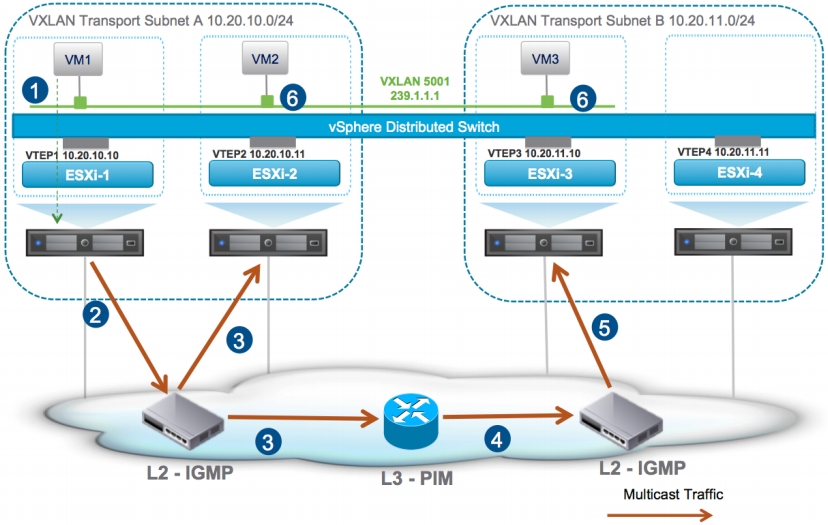
\includegraphics[width=0.5\textwidth]{imaxes/conceptosPrevios/MulticastSeqBUM.png}  \caption{Replicación del tráfico BUM en el modo Multicast}
    %     \label{fig:modoMulticast}
    %     \end{figure}
    %     \FloatBarrier
    %         \item \textbf{Modo Unicast}: no requiere ninguna configuración específica en la capa física y está gestionado por VMware NSX. Se crea un grupo con los VTEP situados en el mismo segmento de red, dentro de cada grupo se selecciona un host ESXi para el rol de \textit{Unicast Tunnel End Point} (UTEP), encargado de recibir el tráfico BUM que procede de otros segmentos de red para reenviarlo por su segmento pero solo a los hosts con al menos una máquina virtual. El host ESXi emisor utiliza la tabla VTEP para comprobar que VTEPs están situados en una VXLAN y así poder dirigir el tráfico BUM correspondiente.\\
    %         Este modo es útil en entornos pequeños donde no hay mucho tráfico y cada segmento de red tiene pocos VTEP.
    %     \begin{figure}[h!]
    %     \centering
    %     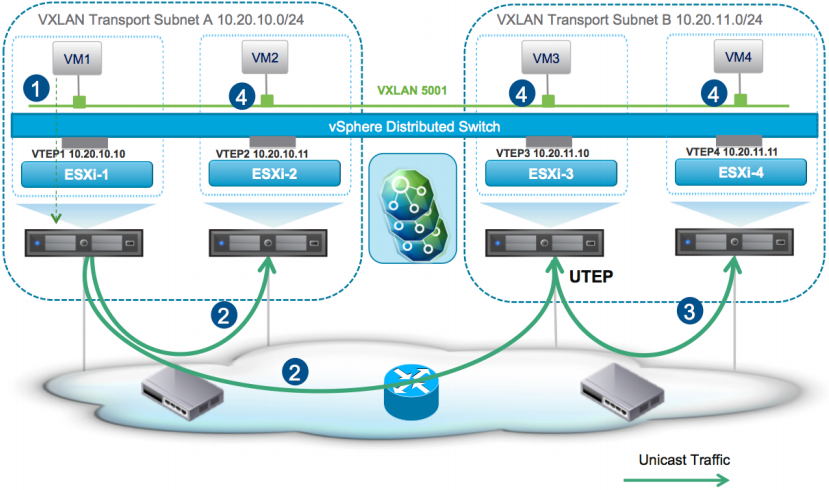
\includegraphics[width=0.5\textwidth]{imaxes/conceptosPrevios/UnicastMode.png}
    %     \caption{Replicación del tráfico BUM en el modo Unicast}
    %     \label{fig:modoUnicast}
    %     \end{figure}
    %     \FloatBarrier
    %         \item \textbf{Modo Híbrido}: combina el modo Unicast y el modo Multicast. El tráfico dirigido a las máquinas virtuales situadas en el mismo segmento de red se transmite usando Multicast, por lo que se requiere tener el protocolo IGMP configurado en los dispositivos físicos de capa 2, se recomienda establecer una dirección Multicast por cada VXLAN. El tráfico se replica a los hosts ESXi que forman parte del grupo. Cuando el tráfico va dirigido a máquinas virtuales situadas en hosts en distinto segmento de red, se transmite utilizando Unicast, como en ese modo, se forma un grupo con los hosts de cada segmento y de cada grupo se elige un host con el rol de \textit{Multicast Tunnel EndPoint} (MTEP). Así, el host que origina el tráfico BUM lo transmite al MTEP correspondiente, el cual se encarga de replicar ese tráfico por su segmento de red. La replicación del tráfico entre segmentos es gestionada por las instancias de NSX Controller.\\
    %         Este modo de replicación permite desplegar NSX en entornos grandes gracias a que el tráfico Multicast y Unicast se pueden escalar facilmente, el primero se reduce a cada segmento de red y la transmisión del segundo en la capa 3 está gestionado por VMware NSX sin necesidad de configurar los dispositivos físicos.
    %     \begin{figure}[h!]
    %         \centering
    %         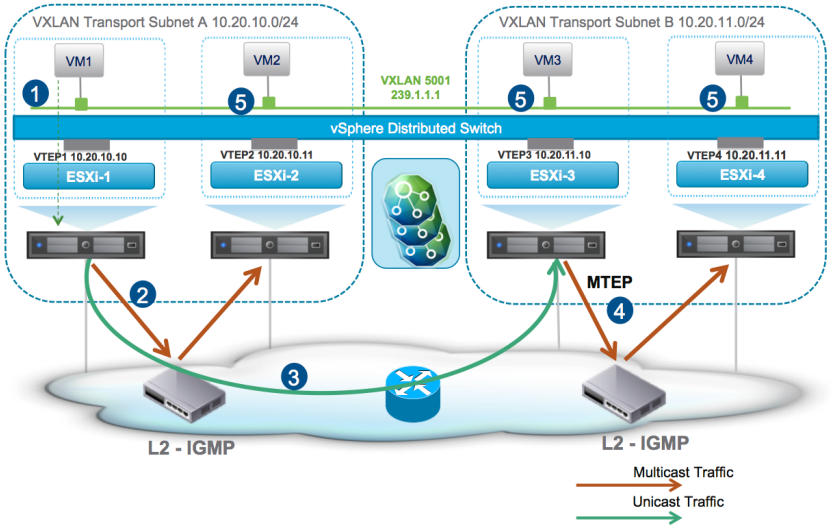
\includegraphics[width=0.5\textwidth]{imaxes/conceptosPrevios/hibrydMode.png}
    %         \caption{Replicación del tráfico BUM en el modo Híbrido}
    %         \label{fig:modoHibrido}
    %     \end{figure}
    %     \FloatBarrier
    %     \end{itemize}
    
    %  El enrutamiento del tráfico está gestionado por dos componentes Distributed Logical Router (DLR) y NSX Edge Services Gateway (ESG). Un mismo DLR se extiende por varios hosts ESXi para enrutar el tráfico entre VXLANs, también mantiene una conexión con las instancias de ESG para transmitir el tráfico que se dirige a redes externas, esa conexión se denomina \textit{transit network} y está getionada por un Logical Switch. Cada DLR tiene su propio Logical Router Control para intercambiar las rutas disponibles con las instancias de ESG, posteriormente, son las instancias de NSX Controller las que transmiten esta información al DLR distribuido en los hosts ESXi. Las interfaces lógicas del DLR conectan con cada Logical Switch, cada interfaz tiene una dirección IP que representa el \textit{gateway} del segmento de red al que esté conectada [Fig. \ref{fig:logicalRoutingCompo} y \ref{fig:redLogicaOne}]. Estos dispositivos utilizan enrutamiento dinámico (protocolos OSPF o BGP).
     
    %  \begin{figure}[h!]
    %   \centering
    %   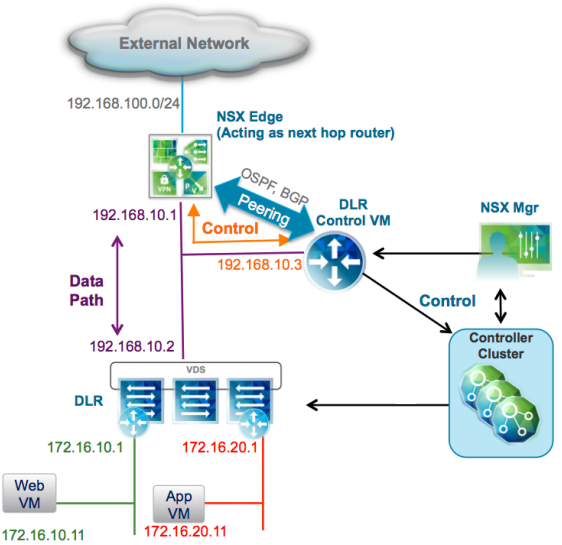
\includegraphics[width=0.4\textwidth]{imaxes/conceptosPrevios/LogicalRoutingComponents.png}
    %   \caption{Componentes de la red virtual que intervienen en el enrutamiento del tráfico.}
    %   \label{fig:logicalRoutingCompo}
    % \end{figure}
    % \FloatBarrier
    
    % \begin{figure}[h!]
    %   \centering
    %   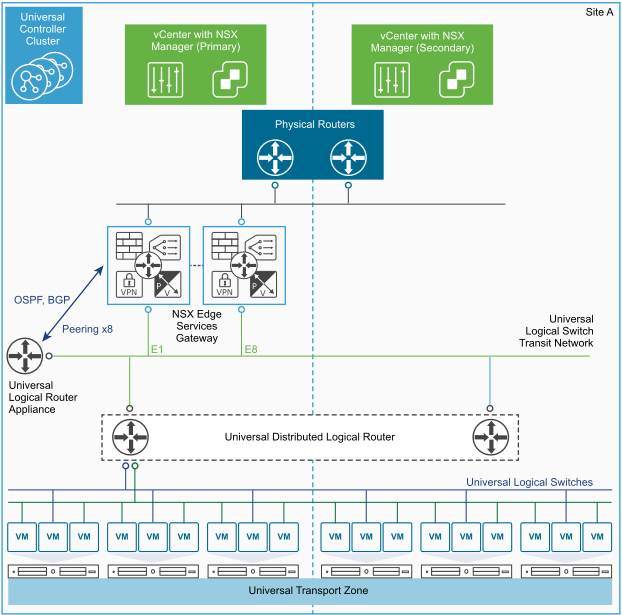
\includegraphics[width=0.5\textwidth]{imaxes/conceptosPrevios/redlogCF.png}
    %   \caption{Red lógica formada en un SDDC con dos clusters.}
    %   \label{fig:redLogicaOne}
    % \end{figure}
    % \FloatBarrier
     
    %  En el SDDC deben existir, al menos, dos intancias de ESG aunque se pueden desplegar hasta 8 instancias. En el modelo consolidado se debe tener un único UDLR para que las rutas entre hosts ESXi sean más cortas, debe existir un Logical Switch que forme la \textit{transit zone}. En el modelo estándar debe existir un UDLR extendido por todos los \textit{Management Cluster} (si hay varias \textit{Regions}), un UDLR extendido por el \textit{Shared Edge and Compute Cluster} y el resto de \textit{Compute Clusters} en cada \textit{Region}, y un DLR extendido por todos los clusters de una misma región.En el modelo estándar existen dos tipos de \textit{transit zones}, una entre el UDLR que atraviesa todas las \textit{Regions} y cada instancia de ESG, y otra que conecta el DLR propio de cada \textit{Region} y sus instancias de ESG. 
    % \\
    % Algunos componentes de VMware Cloud Foundation se deben desplegar en una VXLAN dedicada para proporcionar recuperación ante fallos en caso de que parte del SDDC deje de funcionar. Entre otros componentes (solo vamos a tratar aquellos que son obligatorios), VMware vRealize Log Insight se debe desplegar en una red de este tipo, llamada \textit{Application Virtual Network} (AVN). En entornos con varias \textit{Regions} se crea una \textit{transport zone} que se extiende por todo el SDDC y una \textit{transport zone} adicional en cada \textit{Region}, la primera proporciona recuperación ante fallos a través de todo el SDDC a los componentes que lo requieran, y la segunda solo a través de una \textit{Region}, sin necesidad de reconfigurar direcciones IP o DNS. VMware vRealize Log Insight se debe desplegar en una VXLAN por cada \textit{Region}.
    % \\
    % El acceso a una AVN se realiza a través de las instancias de ESG desplegadas en el entorno, estas se conectan a un UDLR que gestiona el tráfico de la s máquinas virtuales que tiene conectadas. El enrutamiento debe ser dinámico con BGP y las instancias de ESG proporcionan protegen y balacean la carga de trabajo con los servicios de VMware NSX Firewall y Load Balancing [Fig. \ref{fig:avnConsolidated}].\\
    % **VERIFICAR LO DEL LOAD BALANCING en el despliegue. ¿solo para las que son cross-region o tambien en las de una sola region**\\
    % \begin{figure}[h!]
    %   \centering
    %   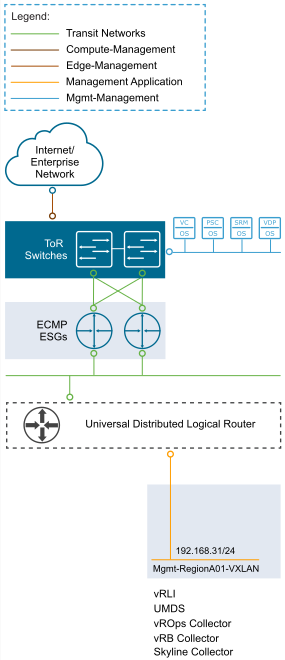
\includegraphics[width=0.25\textwidth]{imaxes/conceptosPrevios/AVNConsolidated.png}
    %   \caption{AVN en el modelo consolidado}
    %   \label{fig:avnConsolidated}
    % \end{figure}
    % \FloatBarrier
    
    % Este utiliza los componentes vCenter Server, NSX Manager, NSX Controllers y NSX Logical Switch para establecer comunicaciones y aislar los distintos tipos de tráfico [Fig. \ref{fig:planosNSX}]. Estos componentes \underline{actúan en diferentes planos} de la red:
    
    
    
    % \begin{itemize}
    %     \item \textbf{Plano de Datos}: esta capa gestiona la transmisión del tráfico entre los componentes del SDDC. En este plano actúan NSX Logical Switches segregando los tipos de datos, y el enrutamiento y firewall distribuído de NSX. Se transmite a través de una red física dedicada al transporte.
    %     \item \textbf{Plano de Control}: aquí se gestionan los mensajes de control que se usan para la configuración de los dispositivos de NSX como switches, routers y firewalls en cada host ESXi. Se distribuye en redes físicas de forma segura usando VLANs para aislarlo del plano de datos.
    %     \item \textbf{Plano de gestión}: aquí se gestiona el tráfico dedicado a la administración de los recursos como puede ser la creación y eliminación de máquinas virtuales. Está controlado por vCenter Server y NSX Manager.
    % \end{itemize}
    % \begin{figure}[h!]
    %   \centering
    %   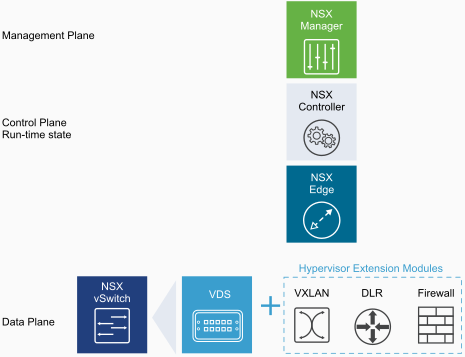
\includegraphics[width=0.65\textwidth]{imaxes/conceptosPrevios/planosNSX.png}
    %   \caption{Como se estructuran las componentes de VMware NSX for vSphere}
    %   \label{fig:planosNSX}
    % \end{figure}
    % \FloatBarrier
    
    %\fi
    
    % \iffalse
    % \subsubsection{Almacenamiento Virtual}
    % VMware vSAN forma único \textit{datastore} con todos los dispositivos de almacenamiento que se encuentran en la infraestructura permitiendo establecer políticas y gestionar esos recursos de forma más simple. Para que funcione correctamente es necesario \underline{configurar una red para VMware vSAN} teniendo en cuenta los siguientes aspectos:
    % \begin{itemize}
    %     \item El uso de vSpehere Distributed Switches genera mejor rendimiento.
    %     \item Se recomienda el uso de paquetes tipo \textit{jumbo frames}.
    %     \item Asignar una VLAN al tráfico de cada cluster de VMware vSAN.
    %     \item Si se implementa en un SDDC con dos localizaciones, es necesario establecer un host \textit{witness}.
    % \end{itemize}
    % Al establecer el tamaño y capacidad de este cluster hay que tener en cuenta que cuantos más hosts ESXi se incluyan, mayor tolerancia a fallos se tendrá y mejor se podrán repartir los grupos de discos entre todos los hosts. Debe haber un balance entre el hardware y la capacidad requerida.
    
    
    % \fi
    \end{subsection}
    
    
    \begin{subsection}{Operaciones de la Arquitectura\cite{CFopermanagement}}
    En este apartado se define como se gestionan en VMware Cloud Foundation las tareas de administración de todas las partes de la infraestructura. Estas tareas se agrupan en la gestión del ciclo de vida y la recopilación de información sobre el estado de cada componente existente.
    
    \subsubsection{Gestión del Ciclo de Vida}
    Elementos que se encargan de administrar el ciclo de vida de los componentes:
    \begin{itemize}
    %     \item \textbf{vSphere Update Manager}: por cada instancia de VMware vCenter Server se despliega una instancia de vSphere Update Manager. Este componente utiliza el servicio \textit{Update Manager Download Service} (UMDS) para obtener las actualizaciones de la red externa al SDDC, el cual se despliega en una red AVN [Fig. \ref{fig:avnConsolidated}], permitiendo limitar el acceso a Internet de vSphere Update Manager y reduciendo el número de descargas ya que un UMDS se comparte entre varias instancias de VMware vCenter Server. Se crea una instancia de UMDS por cada \textit{region} existente [Fig. \ref{fig:UpdateManagerArc}].
    %     \begin{figure}[h!]
    %         \centering
    %         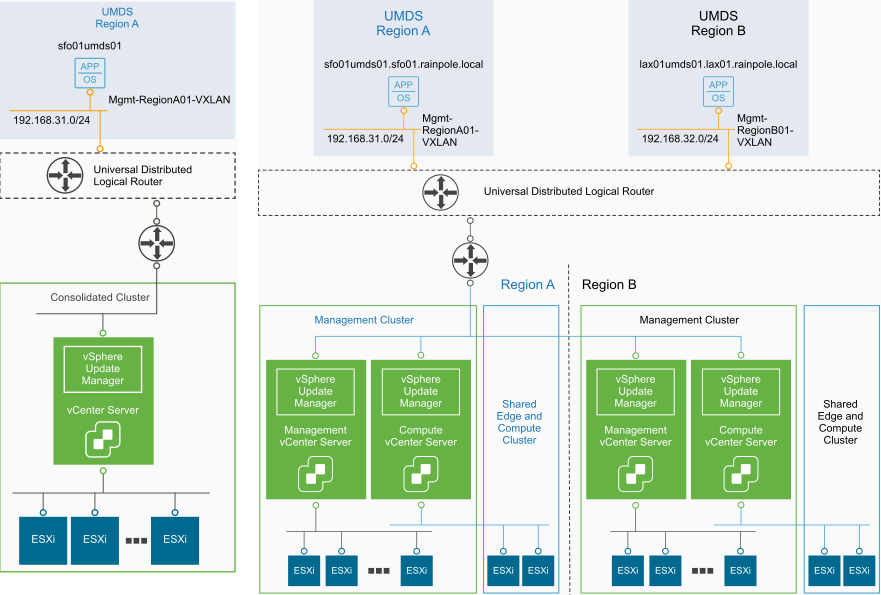
\includegraphics[width=0.5\textwidth]{imaxes/conceptosPrevios/UpdateManagerArch.png}
    %         \caption{Diseño de vSphere Update Manager en el modelo consolidado (izquierda) y en el modelo estándar (derecha)}
    %         \label{fig:UpdateManagerArc}
    %     \end{figure}
    %     \FloatBarrier
        
        \item \textbf{vRealize Suite Licfecycle Manager}: componente utilizado para desplegar, actualizar y configurar, de forma automatizada, los productos vRealize Operations, vRealize Log Insight, vRealize Automation y vRealize Business Cloud. De este componente se despliega una única instancia en una AVN accesible desde cada \textit{region} por todas las instancias de VMware vCenter Server. Se debe registrar su nombre de dominio en el servidor DNS para hacerla accesible.
        
    %     \iffalse
    %     y se puede elegir entre dos modelos de despliegue, uno en el que se usa una máquina virtual denominada  que se encarga de descargar los archivos requeridos por vSphere Update Manager mientras este se encuentra en un entorno aislado [Fig. \ref{fig:updateManager}], y otro donde es la instancia de vSphere Update Manager la que realiza la descarga de los ficheros. La primera opción incrementa la seguridad y permite compartir estos archivos entre distintas instancias de vSphere Update Manager.\\
    %     Una vez desplegado se pueden establecer diferentes configuraciones a nivel de host, máquina virtual y cluster, para que durante la instalación de actualizaciones el servicio del SDDC continúe operativo y evitar la pérdida de información y errores en los recursos.
    %     \begin{figure}[h!]
    %   \centering
    %   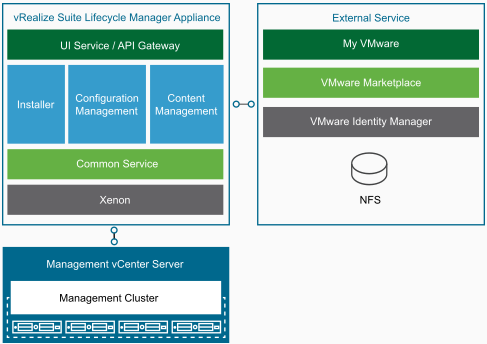
\includegraphics[width=0.8\textwidth]{imaxes/conceptosPrevios/vRealizeUpdateArchLifeCyle.png}
    %   \caption{Estructura de la gestión del ciclo de vida con vRealize Suite Lifecycle Manager.}
    %   \label{fig:vrealizeUpdateManager}
    % \end{figure}
    % \FloatBarrier
    %     \fi
    
    
    \end{itemize}
    
    
    
    
    % \subsubsection{Gestión de Logs}
    % En VMware Cloud Foundation el producto vRealize Log Insight provee gestión y análisis de los logs de la infraestructura. Este componente resgistra los logs, alarmas y eventos de Platform Services Controller, instancias de VMware vCenter Server, de los hosts ESXi, componentes de VMware NSX, vRealize Suite Lifecycle Manager y componentes de vRealize Automation, utilizando el protocolo \textit{syslog} para su obtención. En el modelo consolidado se recomienda desplegar vRealize Log Insight en tamaño reducido, es decir, un solo nodo \textit{master} que gestiona los logs de todos los componentes, pero también se pueden desplegar otros nodos \textit{worker}. Para el modelo estándar se deben desplegar al menos tres nodos por cada \textit{region}, uno \textit{master} y dos \textit{worker}, y el uso de Load Balancer proporciona tolerancia a fallos en caso de que falle uno de los nodos. En ambos modelos los nodos se despliegan en una AVN que solo se extiende por una \textit{region} [Fig. \ref{fig:redLogIsight}], también se deben configurar la dirección IP y nombre de dominio de cada nodo en el servicio DNS.
    %     \begin{figure}[h!]
    %   \centering
    %   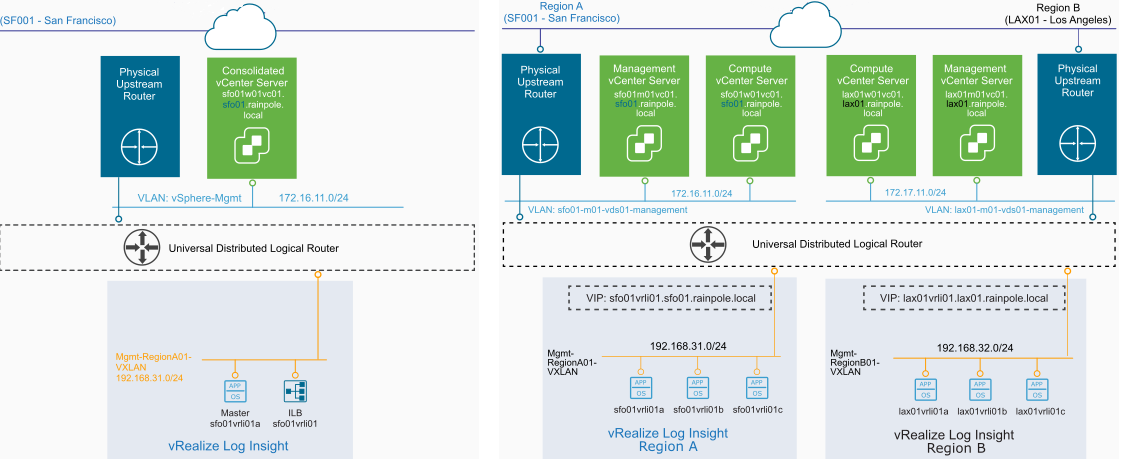
\includegraphics[width=0.7\textwidth]{imaxes/conceptosPrevios/networkLogInsight.png}
    %   \caption{Localización de vRealize Log Insight en el modelo consolidado (izquierda) y en el modelo estándar (derecha)}
    %   \label{fig:redLogIsight}
    % \end{figure}
    % \FloatBarrier
    \end{subsection}
    \end{section}
% \begin{section}{Conceptos}
En este apartado se describen algunos conceptos que se deben tener claros para entender la estructura y arquitectura de los componentes de VMware Cloud Foundation.
% En este apartado se describe la arquitectura de VMware Cloud Foundation y como estructura sus componentes\footnote{Se describen solo aquellos componentes que se utilizarán en el despliegue de Cloud Foundation.} internamente.

%%%%%%%%%%%%%%%%%%%%%%%%%%%%%%
% \iffalse
% En este apartado se explican aquellos conceptos de VMware Cloud Foundation necesarios para entender su funcionamiento, configuración y requisitos de la infraestructura previos al despliegue del servicio.
% \fi
%%%%%%%%%%%%%%%%%%%%%%%%%%%%%%%%


%% Workload Ddomains %&%&%%%%
%%%%%%%%%%%%%%%%%%%%%%%%%%%%
\begin{subsection}{Workload Domain}
Un Workload Domain (WD) representa un bloque de recursos dentro del SDDC, formado por recursos físicos y virtuales, gestionados por los componentes de VCF. En cada WD se despliegan instancias de los componentes de VCF para controlar el acceso y uso de los recursos virtuales y físicos, estableciendo, además, una capa de seguridad sobre el WD. Esto permite que los recursos de cada WD se gestionen de forma separada. La función de un WD consiste en separar flujos de trabajo para determinar que recursos se dedican a la realización de determinadas tareas.
% Un \textit{workload domain} consiste en una instancia lógica de un SDDC que abarca todos o parte de los recursos de uno o más clusters, cuya función es aislar el flujo de trabajo de un usuario, aplicación o un determinado tipo de tareas. Cada \textit{workload domain} se extiende sobre varios hosts con el hipervisor ESXi, y contiene sus propias instancias de VMware vCenter Server, VMware vSAN y VMware NSX-T. Así, esta arquitectura permite establecer políticas de control específicas para un \textit{workload domain} y otras comunes para todos o varios \textit{workload domains} y específicas para cada uno de ellos a la vez que se simplifica la complejidad de la infraestructura. Existen \underline{tres tipos} de \textit{workload domains} que permiten aislar las tareas de gestión de la infraestructura del resto de flujos de trabajo. 

%% MANAGEMENT DOMAIN
\begin{subsubsection}{Management Domain}
\label{subsubsec:domainManagement}
% Este \textit{workload domain} se crea y configura automáticamente durante el proceso de despliegue de una instancia de VMware Cloud Foundation.
El Management Domain es el primer WD que se crea dentro del SDDC cuando se despliega VCF. Su finalidad es alojar todos los componentes de VCF que gestionan el propio Management Domain y al resto de WDs. Inicialmente, se despliegan las siguientes VMs de cada componente:

\begin{itemize}
  \item Una VM de SDDC Manager.
  \item Una VM de VMware vCenter Server.
  \item Tres VMs de VMware NSX-T Manager Appliance.
  \item Dos VMs de VMware NSX-T Edge.
\end{itemize}
Al contener todas las instancias de los componentes dedicados a la gestión del SDDC, todas las tareas de administración suceden dentro de este WD. De esta forma, su ejecución está centralizada, es más segura y está mejor controlada, ya que lo hacen sobre un conjunto de recursos dedicados exclusivamente a ellas.
% El administrador gestiona los recursos del Management Domain, tanto hosts como instancias de los componentes, desde VMware vSphere Client, y VMware NSX-T Manager se encarga de controlar y mantener las redes virtuales del SDDC. Con VMware SDDC Manager, el administrador gestiona de forma centralizada los aspectos que afectan al ciclo de vida de todos los componentes del SDDC.


% Incluye las siguientes instancias: SDDC Manager, vCenter Server, una instancia de NSX Manager, tres instancias de NSX Controller, dos instancias de Platform Services Controller y tres instancias de vRealize Log Insight \cite{sddcComponents} [Fig. \ref{fig:componentsMNGDomain}].\\
% Cuando se \underline{despliega \textit{management domain} se crean y configuran} de forma automatizada por SDDC Manager las siguientes máquinas virtuales (VM) de cada componente de Cloud Foundation\footnote{Las características de cada máquina virtual se refieren a los requisitos mínimos}:
% \begin{itemize}
%     \item Una VM de \textbf{SDDC Manager}: 4 vCPU, 16 GB de memoria, 800 GB de almacenamiento.
%     \item Una VM de \textbf{vCenter Server}: 4 vCPU, 16 GB de memoria, 290 GB de almacenamiento.
%     \item Dos instancias de \textbf{Platform Services Controller} (cada una): 2 vCPU, 4 GB de memoria, 60 GB de almacenamiento.
%     \item Una VM de \textbf{NSX Manager}: 4 vCPU, 16 GB de memoria, 60 GB de almacenamiento.
%     \item Tres VM de \textbf{NSX Controller} (cada una): 4 vCPU, 4 GB de memoria, 28 GB de almacenamiento.
%     \item Tres VM de \textbf{vRealize Log Insight}: 4 vCPU, 8 GB de memoria, 250 GB de almacenamiento.
% \end{itemize}

% Para desplegar el \textit{management domain} se requieren las siguientes \underline{capacidades mínimas} en la infraestructura \cite{WDminRequierements}:
% \begin{itemize}
%     \item \textbf{Hosts}: 4
%     \item \textbf{CPU} por host: Dual-socket con 8 cores por socket, en sistemas All-Flash.
%     \item \textbf{Memoria} total: 192 GB
%     \item \textbf{Almacenamiento} por host: 16 GB para el dispositivo de arranque, un NVMe o SSD para la capa de caché, dos SSD o HDD para la capa de capacidad\footnote{En total se requieren 800 GB para este \textit{workload domain}.}.
%     \item \textbf{NICs} por host: Dos NICs de al menos 10 GbE y, opcionalmente un NIC 1GbE BMC.
% \end{itemize}

% \begin{figure}[h!]
%   \centering
%   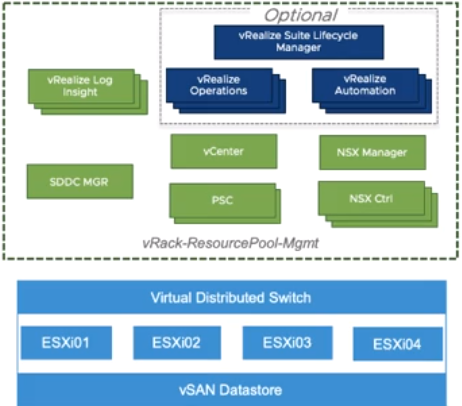
\includegraphics[width=0.5\textwidth]{imaxes/conceptosPrevios/componentsMANAGEDomain.png}
%   \caption{Componentes de \textit{management domain}}
%   \label{fig:componentsMNGDomain}
% \end{figure}
\end{subsubsection}

%% VIRTUAL INF. DOMAIN
\begin{subsubsection}{Virtual Infrastructure Domain (VI)}
\label{subsubsec:domainVI}
Este tipo de WD se crea manualmente y bajo demanda desde el Management Domain, para habilitar un entorno, cuyos recursos puedan ser usados por los usuarios mediante el despliegue de aplicaciones. Su configuración de hardware y lógica se especifican durante el proceso de creación, pudiendo establecer la cantidad de hosts, cantidad de almacenamiento, configuración de la red y políticas de rendimiento y disponibilidad, todo para satisfacer las necesidades del tipo de tareas que se van a realizar en él. Con la creación de un WD se generan las siguientes VMs:
% Con cada WD se genera un nuevo cluster de VMware vSphere que agrupa los nuevos recursos, aunque parte de sus componentes que se despliegan se controlan desde el Management Domain:
\begin{itemize}
  \item Una VM de VMware vCenter Server que se sitúa en el Management Domain.
  \item Tres VMs de VMware NSX-T Manager Appliance situadas en el Management Domain.
  \item Dos VMs de VMware NSX-T Edge.
\end{itemize}
Que ciertos componentes se sitúen en el Management Domain, permite separar las tareas de administración de un VI Domain de las aplicaciones y recursos de los usuarios, haciendo un entorno mejor organizado, más seguro y óptimo.

% El administrador gestiona los recursos del VI Domain desde VMware vSphere Client y la instancia de SDDC Manager situada en el Management Domain, y gestiona las redes virtuales del WD desde VMware NSX-T Manager situado también en el Management Domain. Los usuarios despliegan sus aplicaciones sobre los recursos de este WD, de esta forma, las tareas administrativas y las de consumo se ejecutan desde entornos separados.
% La diferencia entre un \textit{virtual infrastructure domain} y \textit{virtual desktop infrastructure domain} es que el segundo incorpora el producto VMware Horizon View que, resumiendo, permite desplegar escritorios virtuales. 
% Con cada nuevo \textit{virtual infrastructure domain} se crea un nuevo cluster vSphere en la infraestructura que agrupa todos los recursos que tiene asignados.\\
% Cuando se \underline{despliega un \textit{virtual infrastructure domain} se crean y configuran} de forma automatizada por el componente SDDC Manager las siguientes máquinas virtuales (VM) de cada componente de VMware Cloud Foundation\footnote{Las características de cada máquina virtual se refieren a los requisitos mínimos} 
%\cite{sddcComponents} [Fig. \ref{fig:compoVIdomain}]:
% \begin{itemize}
%     \item Una VM de \textbf{vCenter Server} en Management Domain: 8 vCPU, 24 GB de memoria, 500 GB de almacenamiento.
%     \item Una VM de \textbf{NSX Manager} en Management Domain: 4 vCPU, 16 GB de memoria, 60 GB de almacenamiento.
%     \item Tres VM de \textbf{NSX Controller} en el VI Domain creado (cada una):  4 vCPU, 4 GB de memoria, 28 GB de almacenamiento.
% \end{itemize}

% Por cada \textit{virtual infraestructure domain} que se despliega en la infraestructura, se requieren las siguientes capacidades mínimas\cite{WDminRequierements}:
% \begin{itemize}
%     \item \textbf{Hosts}: 3
%     \item \textbf{CPU}, \textbf{Memoria} y \textbf{Almacenamiento}: depende de los requisitos de las tareas que se vayan a desarrollar en este \textit{workload domain}.
%     \item \textbf{NICs} por servidor: Dos NICs de al menos 10 GbE y, opcionalmente un NIC 1 GbE BMC.
% \end{itemize}


 \end{subsubsection}

\end{subsection}
% \begin{figure}[h!]
%   \centering
%   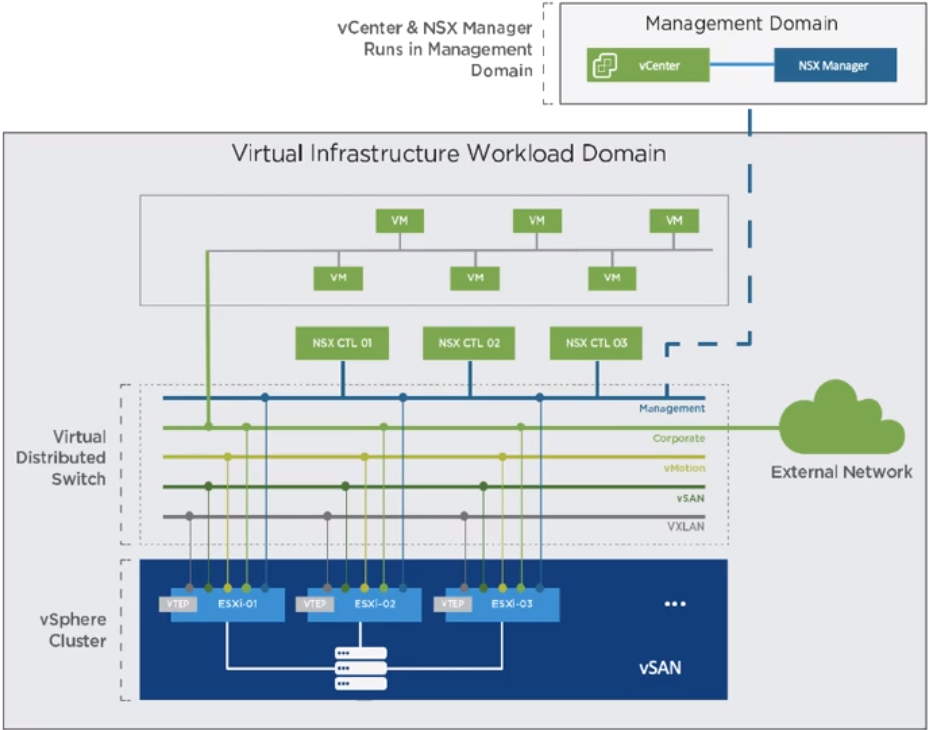
\includegraphics[width=0.5\textwidth]{imaxes/conceptosPrevios/networkArcVIDomain.png}
%   \caption{Componentes de \textit{virtual infrastructure domain}.}
%   \label{fig:compoVIdomain}
% \end{figure}
%\FloatBarrier

%&%%%%%%%%%%%%%%%%%%%%%%%%%%%%%%%%%%%%%%%%%%%%%%%%%%%%%%%%
%% ARQUITECTURA



\begin{subsection}{Arquitectura}
VMware proporciona dos posibles modelos de arquitectura diferentes. Se utiliza uno u otro dependiendo del tamaño de la infraestructura sobre la que se va a desplegar VCF, y con cada modelo, se determina la forma en la que se agruparán y administrarán los recursos del SDDC.

%%%%%%%%%%%%%%%%%%%%%
%%%%%%%%%%%%%%%%%%%%%%%%
%% ESTANDAR
\begin{subsubsection}{Modelo estándar}

Este modelo está pensado para entornos de tamaño medio/grande, con un mínimo de siete hosts. Está formado por un Management Domain y al menos un VI Domain. Esto implica que la ejecución de tareas dentro de un WD está limitada por los recursos que lo forman. Esto permite asignar roles a los recursos según las operaciones que se van a ejecutar sobre ellos, establecer un nivel de seguridad en cada WD y dedicar un conjunto de recursos a la ejecución de cierto tipo de operaciones. Así, el entorno es más eficiente, ya que se proporciona una forma de adecuar la configuración de los recursos de acuerdo con el uso que se va a hacer del servicio o servicios desplegados, minimizando además los cambios sobre la infraestructura física.
% esde el Management Domain se administra toda la infraestructura del SDDC y cada VI Domain existente, los cuales son creados bajo demanda desde el Management Domain y sus recursos se establecen según su finalidad. Un Management Domain puede gestionar hasta un máximo de de catorce VI Domain. 
%Cada \textit{virtual infrastructure domain} requiere tres hosts adicionales, es decir, un host solo puede pertenecer a un único \textit{workload domain}. 

\begin{figure}[h!]
  \centering
  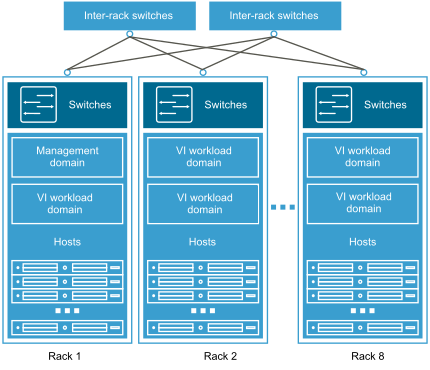
\includegraphics[width=0.6\textwidth]{imaxes/conceptosPrevios/arquitect_standarCF.png}
  \caption{Esquema del modelo de arquitectura estándar.}
  \label{fig:modelostandard}
\end{figure}

% \begin{figure}[h!]
%   \centering
%   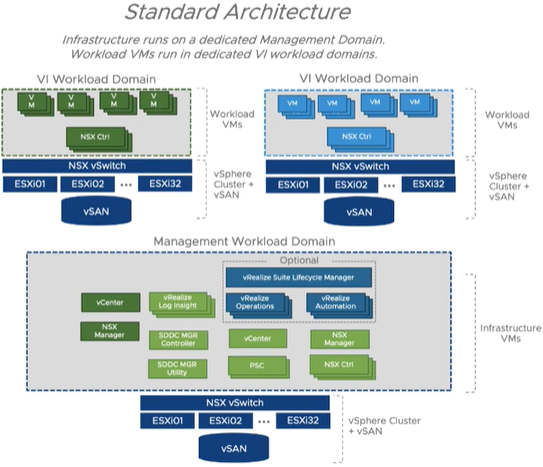
\includegraphics[width=0.6\textwidth]{imaxes/conceptosPrevios/standardArch.png}
%   \caption{Estructura de los componentes en una arquitectura estándar.}
%   \label{fig:standardarch}
% \end{figure}
\FloatBarrier
%%%%%%%%%%%%%%%%%%%%%
%%  CONSOLIDADO
\end{subsubsection}
\begin{subsubsection}{Modelo consolidado}
Este modelo está orientado a entornos de tamaño pequeño, con menos de siete hosts. Está formado por un único WD que cumple las funciones de un Management Domain y de un VI Domain, es decir, en él se colocan las instancias de los componentes dedicados a la gestión del SDDC\footnote{Se despliega la misma cantidad de instancias que en el Management Domain.} junto con las aplicaciones desplegadas para la realización de otro tipo de tareas. Así, a diferencia del modelo estándar, todas las operaciones se ejecutan dentro de un mismo entorno y sobre los mismos recursos. Internamente, las VMs se pueden colocar dentro de un grupo, llamado \textit{resource pools}, en el que se puede establecer un límite de uso de recursos.
Este modelo no aporta tantos beneficios como el modelo estándar, ya que todas las operaciones se realizan sobre los mismos recursos, y los niveles de control y seguridad son menores, por lo tanto su uso solo está recomendado para entornos de tamaño reducido.
% Dentro del cluster de VMware vSphere que se crea, las instancias pertenecientes a los componentes de administración del SDDC y las pertenecientes al trabajo de los usuarios, se colocan en \textit{resource pools} separados. Un \textit{resource pool} es un elemento de VMware vSphere que permite establecer unos límites de consumo de recursos sobre las instancias que se sitúan en su interior\cite{resourcePool}.

% Este modelo está pensado para desplegar VMware Cloud Foundation en entornos de tamaño pequeño, normalmente cuando hay menos de siete hosts, aunque también se puede utilizar en entornos más grandes con hasta 64 hosts. En este modelo los flujos de trabajo que corresponden al \textit{virtual infrastructure domain} y al \textit{management domain} en el despliegue estándar, están colocados dentro de un mismo \textit{workload domain} en un único cluster pero aislados gracias a que cada uno se coloca dentro de un \textit{resource pool} diferente, es decir, existe un cluster con varios \textit{resource pool}. El modelo consolidado se convierte en un modelo estándar cuando se añade un \textit{workload domain} al SDDC.[Fig. \ref{fig:modeloconsolidated}].

\begin{figure}[h!]
  \centering
  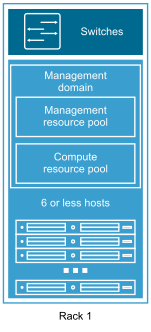
\includegraphics[width=0.25\textwidth]{imaxes/conceptosPrevios/modelConsolidated.png}
  \caption{Esquema del modelo de arquitectura consolidado.}
  \label{fig:modeloconsolidated}
\end{figure}

% \begin{figure}[h!]
%   \centering
%   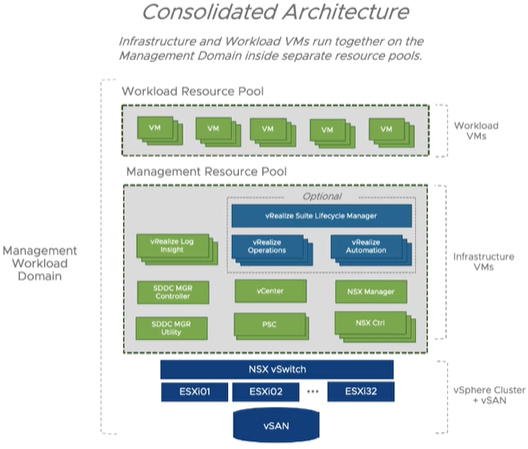
\includegraphics[width=0.6\textwidth]{imaxes/conceptosPrevios/consolidatedArch.png}
%   \caption{Estructura de los componentes de una arquitectura consolidado.}
%   \label{fig:consolidatedArch}
% \end{figure}
\FloatBarrier

\end{subsubsection}
\end{subsection}

\begin{subsection}{Clusters, zonas y distribución de un SDDC}

  Los recursos de un SDDC pueden estar distribuidos en diferentes localizaciones para proporcionar mayor disponibilidad y recuperación ante fallos. Estos recursos, se agrupan para formar una estructura que permite usar y gestionar los recursos disponibles de forma conjunta y dinámica.

\begin{subsubsection}{Availability Zone, Region y Cluster}
\begin{itemize}
  \item Availability Zone (AZ): se llama AZ a un conjunto de recursos físicos que forman una infraestructura independiente, es decir, cada una tiene su propia fuente de energía, su sistema de refrigeración, su sistema de seguridad y su red, no compartidos con otra AZ, para evitar la propagación de fallos hacia otras AZs. Cuando existen varias AZs, se pueden usar de forma que cuando ocurre un fallo en una de ellas la carga de trabajo se distribuye a una segunda AZ y, así, minimizar el tiempo de caída del servicio. Dentro de una AZ se alojan uno o más WDs.
  
  \item Region: se llama Region a un conjunto de AZs situadas en una misma ubicación, es decir, las AZs de una Region están situadas próximas entre sí. Estas AZs deben tener al menos una latencia de 5 ms entre ellas. Dentro de un SDDC pueden existir varias Regions pero estas se sitúan en ubicaciones más distantes, la latencia debe ser de al menos 150 ms. Esta estructura permite ofrecer los servicios de un SDDC en diferentes ubicaciones, a la vez que se aumenta su disponibilidad y recuperación ante fallos.
  
  \item Cluster: un cluster de VMware vSphere es una agrupación de hosts. A las instancias desplegadas sobre ellos, se les aplica una configuración de disponibilidad con el componente VMware vSphere, permitiendo determinar como se restablecen las instancias cuando ocurre un fallo dentro del cluster. Un cluster se sitúa dentro de un WD, por lo tanto, sus recursos estarán limitados por el alcance del WD. 
  %  Esta estructura permite acercar el servicio a ubicaciones separadas por grandes distancias. La arquitectura del modelo consolidado solo soporta una Region con una AZ, mientras que el modelo estándar permite desplegar múltiples Regions con múltiples AZs.
\end{itemize} 

\begin{figure}[h!]
  \centering
  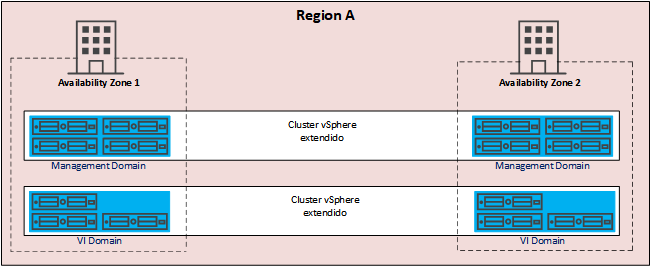
\includegraphics[width=0.8\textwidth]{imaxes/conceptosPrevios/AZRegionCluster.png}
  \caption{Ejemplo de un SDDC con dos Regions y una AZ en cada uno.}
  \label{fig:az-region-cluster}
\end{figure}
En la figura anterior se describe el esquema de un SDDC compuesto de una Region. Dentro de esta, existen dos AZ, AZ1 y AZ2. Cada una de las AZs contiene dos WD, un Management Domain desde donde se administra el SDDC, y un VI Domain donde se realizan las operaciones del SDDC. Como se mencionaba anteriormente, las instancias situadas en una AZ pueden migrar de una ubicación a otra en caso de fallo de los recursos físicos. Para ello, el WD donde se encuentran esas instancias debe estar extendido en las dos AZs. En la imagen, el Management Domain está formado por ocho hosts, repartidos en las AZs, los cuales están agrupados dentro del mismo cluster de VMware vSphere, por lo tanto, los componentes cuyas instancias estén situadas en este cluster se podrán migrar entre los 8 hosts. Estas migraciones se realizan en función de la configuración de disponibilidad establecida en los componentes VMware vSphere y VMware vSAN. Así, cuando los hosts de AZ1 sufren una caída, la AZ2 seguiría activa y las instancias situadas en AZ1 migrarían a AZ2 para continuar la disponibilidad del servicio, todo esto de forma automatizada, dinámica y transparente para el usuario. Lo mismo sucedería con el VI Domain\footnote{Se puede encontrar una descripción más detallada de esta estructura en el siguiente enlace \url{https://docs.vmware.com/en/VMware-Validated-Design/6.0/introducing-vmware-validated-design/GUID-661B1CE3-1F74-4E00-80F3-0F5EA39528CD.html}}.


\end{subsubsection}
% \begin{subsubsection}{Cluster y Resource Pool}
% Dentro de un \textit{workload domain} pueden existir varios clusters. Un cluster es una agrupación de hosts a cuyos recursos se les puede aplicar una una configuración de disponibilidad determinada con los componentes VMware vSphere High Availability y VMware vSphere Distributed Resource Scheduler para establecer como se restablece el servicio en caso de fallos en alguno de los hosts. Un cluster puede estar extendido en más de una AZ para que si una de las AZs falla, las aplicaciones que corrían en ella pueden ser migradas a otra AZ mejorando la disponibilidad del servicio. En un WD se despliegan dos clusters:
% \begin{itemize}
%   \item Management cluster: es el cluster que se crea al desplegar VMware Cloud Foundation. Contiene los componentes para administrar los recursos del WD.
%   \item Shared Edge and Workload Cluster: después del management cluster, este es el primero que se crea. Su finalidad es alojar las aplicaciones y cargas de trabajo de los usuarios dentro de un WD. Además contiene instancias de Vmware NSX-T para proporcionar sevicios de red.
% \end{itemize}

% Dentro de un cluster se pueden crear resource pools. Un \textit{resource pool} es una característica de VMware vSphere que permite abstraer un conjunto de recursos de un cluster estableciendo unos límites de capacidad que puede usar \cite{resourcePool}. Usar resource pools permite agrupar las VMs con una finalidad similar y controlar la cantidad de recursos del WD que esas VMs pueden consumir.

% Un SDDC puede estar distribuído en una o más \textit{Availability Zone} (AZ). Estas son zonas aisladas con infraestructuras independientes que evitan la propagación de fallos de hosts individuales a través de toda la infraestructura, cuantas más \textit{AZ} existan mayor disponibilidad tendrá el servicio. La latencia entre dos \textit{AZ} debe ser de 5 ms como máximo y la conexión de al menos 10 Gbit. Una \textit{Region} agrupa una o más \textit{AZ}s, con esto se da solución a la recuperación del servicio ante desastres. La latencia entre dos \textit{Region}s debe ser de 100 ms como máximo. El \underline{modelo consolidado} solo da soporte a una \textit{Region} con una \textit{AZ}, mientras que el \underline{modelo estándar} puede soportar múltiples \textit{Region} con múltiples \textit{AZ}.
% \end{subsubsection}
\end{subsection}

\end{section}

% \subsubsection{Clusters, zonas de disponibilidad y regiones}
% Un SDDC puede estar formado por uno o más clusters de distintos tipos. En el  \underline{modelo consolidado} la infraestructura está formada por un único cluster que incluye los servicios de gestión de VMware Cloud Foundation VMware vCenter Server, vSphere Update Manager, VMware NSX Manager, VMware NSX Controller y VMware vRealize Log Insight, los servicios de red necesarios para establecer conectividad en el entorno y las máquinas virtuales que los usuarios crean cuando aprovisionan sus recursos. Se aplican las mismas políticas de alta disponibilidad y gestión del ciclo de vida al flujo de trabajo de gestión del SDDC y al flujo de trabajo del usuario. En el \underline{modelo estándar} los distintos \textit{workload domain} se dividen en clusters que pueden ser de tres tipos:
%     \begin{itemize}
%         \item \textbf{Management Cluster}: se crea durante el despliegue de VMware Cloud Foundation y contiene el \textit{management domain}, desde aquí se gestiona el SDDC. Contiene los servicios de gestión mecionados anteriormente.
%         \item \textbf{Shared Edge and Compute Cluster}: es el primer cluster que se crea dentro de un \textit{virtual infrastructure domain} ya que puede haber más de un cluster. Este cluster contiene los servicios de red NSX del \textit{workload domain} y también puede contener el flujo de trabajo de los usuarios.
%         \item \textbf{Compute Cluster}: cluster adicional que se crea dentro de un \textit{virtual infraestructure domain}. Contiene el flujo de trabajo de los usuarios.
%     \end{itemize}
% Un SDDC puede estar distribuído en una o más \textit{Availability Zone} (AZ). Estas son zonas aisladas con infraestructuras independientes que evitan la propagación de fallos de hosts individuales a través de toda la infraestructura, cuantas más \textit{AZ} existan mayor disponibilidad tendrá el servicio. La latencia entre dos \textit{AZ} debe ser de 5 ms como máximo y la conexión de al menos 10 Gbit. Una \textit{Region} agrupa una o más \textit{AZ}s, con esto se da solución a la recuperación del servicio ante desastres. La latencia entre dos \textit{Region}s debe ser de 100 ms como máximo. El \underline{modelo consolidado} solo da soporte a una \textit{Region} con una \textit{AZ}, mientras que el \underline{modelo estándar} puede soportar múltiples \textit{Region}s con múltiples \textit{AZ}s.

%%%%%%%%%%%%%%%%%%%%%%%%%%%%%%%%%%%%%%%%%%%%
%%%%%%%%%%%%%%%%%%%%%%%%%%%%%%%%%%%%%%%%%%%%
%%%%%%%%%%%%%%%%%%%%%%%%%%%%%%%%%%%%%%%%%%%%
% \iffalse
% Un SDDC puede estar \underline{formado por múltiples clusters} que pueden ser de diferentes tipos con diferentes propósitos. Un cluster puede ocupar uno o más \textit{racks} dependiendo del nivel de escalabilidad que se requiera. Según su función, cada \textit{workload domain} se puede colocar en un cluster diferente para gestionar la alta disponibilidad y el ciclo de vida según sus necesidades. Un \underline{cluster puede ser de varios tipos}:
% \begin{itemize}
%     \item \textbf{Management Cluster}: Es aquel que contiene el \textit{management domain}, por lo tanto contiene las máquinas virtuales de los componentes que gestionan el SDDC. A este cluster solo deben acceder los administradores de la infraestructura.
%     \item \textbf{Shared Edge y Compute Cluster}: contiene el \textit{virtual infrastructure domain} con las máquinas virtuales de los usuarios y, además, incorpora servicios de NSX necesarios para comunicarse con redes externas y con otros \textit{workload domains}.
%     \item \textbf{Compute Cluster}: solo contiene el \textit{virtual infrastructure domain} con las máquinas virtuales de los usuarios.
%     \item \textbf{External Storage}: se centra en proveer almacenamiento de tipo NFS, iSCSI o Fiber Channel.
% \end{itemize}

% Un SDDC puede estar distribuído en una o más \underline{zonas de disponibilidad}. Estas son zonas aisladas que evitan la propagación de fallos de hosts individuales a través de toda la infraestructura, así, se puede entregar mayor disponibilidad de los recursos y servicios. A su vez, varias \underline{zonas de disponibilidad} se pueden agrupar en una \underline{región}, estos entornos separados por grandes distancias que permiten tener recuperación ante desastres [Fig. \ref{fig:AVRegiones}].\\

% \begin{figure}[h!]
%   \centering
%   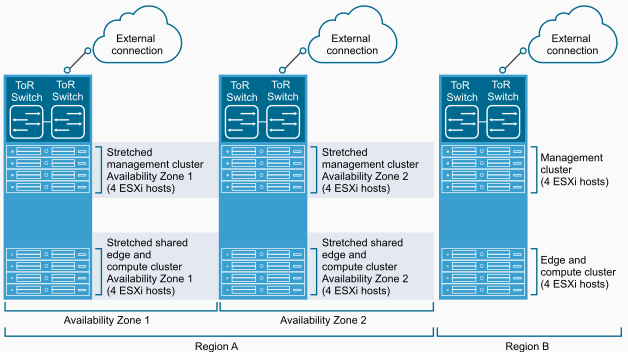
\includegraphics[width=0.95\textwidth]{imaxes/conceptosPrevios/zonasDispRegiones.png}
%   \caption{Una región contiene al menos una zona de disponibilidad.}
%   \label{fig:AVRegiones}
% \end{figure}
% \fi
%%%%%%%%%%%%%%%%%%%%%%%%%%%%%%%%%%%%%%%%%%%%%
%%%%%%%%%%%%%%%%%%%%%%%%%%%%%%%%%%%%%%%%%%%%%
%%%%%%%%%%%%%%%%%%%%%%%%%%%%%%%%%%%%%%%%%%%%%



\begin{section}{Requisitos}
En este apartado se describe aquello que debe cumplir la infraestructura física para que los componentes de VMware Cloud Foundation funcionen de forma adecuada y que la configuración y mantenimiento de los componentes físicos sea sencilla a la hora de expandir el entorno.

% Teniendo en cuenta las capacidades físicas de la infraestructura, se ha elegido el modelo consolidado para el despliegue de VMware Cloud Foundation sobre la infraestructura.     La principal razón por las que se escoge este modelo es por el número de hosts ESXi.
% En los siguientes apartados se describen la arquitectura que se genera y la infraestructura requerida en cada capa.
%%%%%%%%%%%%%%%%%%%%%%%%%%%%%%%%%%%%%%
\begin{subsection}{Cómputo}
\begin{subsubsection}{Hosts ESXi}
    Para realizar el despliegue del primer WD (el Management Domain) se requieren al menos cuatro hosts ESXi con al menos 128 GB de memoria RAM y un disco de arranque de 32 GB cada uno\footnote{Según la configuración establecida para el producto vSAN ReadyNode \cite{host-requirements}}. Para cada WD adicional solo se requiere un mínimo de tres hosts cuya cantidad de memoria RAM depende de la finalidad del WD. Cada uno de los hosts debe tener al menos dos interfaces de red físicas (NIC) que soporten al menos 10 Gbit/seg de velocidad.
    
\end{subsubsection}
\end{subsection}
%%%%%%%%%%%%%%%%%%%%%%%%%%%%%%%%%%%%%%%
\begin{subsection}{Almacenamiento}
    En el Management Domain es obligatorio el uso de un \textit{datastore} de VMware vSAN, este necesita al menos tres hosts con recursos de almacenamiento para funcionar\footnote{VMware vSAN requiere un mínimo de tres hosts mientras que el Management Domain requiere un mínimo de cuatro hosts.}. Se debe aplicar la configuración All-Flash con discos SSD. Basándose en los perfiles que VMware establece para su producto vSAN Ready Node\cite{host-requirements}, cada host debe tener al menos un grupo de dos discos donde la cantidad de almacenamiento para la capa de capacidad debe ser de 4 TB y para la capa de caché de 200 GB. VMware vSAN soporta discos con adaptadores SAS, SATA o SCSI y estos pueden estar configurados en modo \textit{pass-through} o RAID 0. En cuanto a esto, es preferible que los discos se configuren en modo \textit{pass-through} ya que permite que estos se puedan gestionar de forma independiente, sin tener que apagar los hosts cuando sea necesario retirar o añadir discos.
    Para WDs adicionales se puede utilizar almacenamiento NFS en lugar de un datastore de VMware vSAN, aunque la solución de VMware aporta mayor rendimiento y simplifica la administración de esta parte de la infraestructura física.
    % los discos de caché debe ser al menos un 10\% del tamaño total de los discos de capacidad,  y  \footnote{La capacidad de los discos descrita es la necesaria para desplegar el \textit{management domain} y un \textit{workload domain} adicional.}
\end{subsection}
%%%%%%%%%%%%%%%%%%%%%%%%%%%%%%%%%%%%%%%
\begin{subsection}{Red}
 \begin{subsubsection}{Switch Top Of Rack}
     Los hosts están colocados en racks, en un rack puede haber hosts pertenecientes a distintos WD. Para favorecer la alta disponibilidad y tolerancia a fallos de la infraestructura física, un rack debe tener dos switches Top Of Rack (TOR) y cada host debe tener una interfaz conectada a cada uno de ellos, una capa superior de switches conecta los switches TOR entre sí. Todas las conexiones de la red física deben soportar \textit{Jumbo frames} (MTU hasta 9000 Bytes), etiquetado \textit{Quality of Service} (QoS) de tráfico y el etiquetado VLAN, todo para dar soporte a las subredes del SDDC. Todas las conexiones físicas deben tener, al menos, 10 Gbit/seg de velocidad.
    % Todos los switches TOR deben tener al menos dos interfaces 10 Gbit Ethernet como mínimo. 
    % \footnote{Para el Management Domain, las subredes cuya VLAN debe ser configurada en la red física son la subred Management para tareas de administración, la subred dedicada a VMware vSAN, la subred dedicada a overlay y la subred dedicada a VMware vSphere vMotion.}
 \end{subsubsection}
 \begin{subsubsection}{Servicios}
     En el SDDC se deben habilitar varios servicios requeridos por los componentes de VMware Cloud Foundation para su correcto funcionamiento.
     \begin{itemize}
         \item DNS: servidor de nombres para resolver todas las direcciones IP y \textit{hostnames} de los componentes del SDDC.
         \item DHCP: servidor para asignar de forma automática una dirección IP a los hosts que forman el SDDC.
         \item NTP: servidor de tiempo para sincronizar la hora de todos los componentes del SDDC.
         \item Router: se requiere para enrutar el tráfico que emiten todas las instancias del SDDC y para dar acceso a redes externas. Debe soportar enrutamiento dinámico BGP y debe tener configuradas las subredes y VLANS que se vayan a utilizar en la infraestructura.
         \item SMTP: servidor de correo utilizado para el envío de alertas y comunicación de los usuarios con el administrador del SDDC.
         \item Active Directory: servidor de usuarios y grupos de usuarios que el SDDC utiliza como fuente para configurar el acceso a cada parte de la infraestructura virtual.
         \item Certificate Authority: se debe configurar una autoridad certificadora que genere certificados firmados para cada uno de los componentes de VMware Cloud Foundation. Permite establecer conexiones seguras cuando se accede a los componentes.
     \end{itemize}
 \end{subsubsection}
\end{subsection}


\end{section}
%%%%%%%%%%%%%%%%%%%%%%%%%%%%%%%%%%%%%%%
    %%%% DISEÑO ARQUI. FÍSICA %%%%%
% \begin{subsection}{Arquitectura e Infraestructura Físicas \cite{CFfisInfraestuctura}}
%     En este apartado se describen las principales características que tiene el entorno físico de un SDDC construído con VMware Cloud Foundation.


% \begin{subsubsection}{Red física}
% La topología de red en la capa física del SDDC de VMware Cloud Foundation se puede implementar mediante servicios de \underline{transporte} en la capa 2 o en la capa 3. El \underline{diseño en la capa 2} implica que la topología de la red incluya los dispositivos de capa 2 (\textit{Top of Rack Switches}) y los dispositivos de la capa 3 (routers, switches) [Fig. \ref{fig:transportlayer2}], por lo tanto las VLANs que se definan se deben implementar en la capa 2 y en la capa 3. Esto puede provocar problemas al aumentar el tamaño de la red ya que el número de VLANs disponible es más limitado, y problemas de compatibilidad ya que es posible que los dispositivos físicos tengan que ser del mismo proveedor. El \underline{diseño en la capa 3} implica que la topología de la red solo incluye a los dispositivos de capa 3 [Fig. \ref{fig:transportlayer3}]. Esto permite limitar la definición de VLANs a esa capa y el uso de enrutamiento dinámico con protocolos OSPF o BGP entre la capa 2 y 3. Así se consigue una mayor libertad a la hora de seleccionar los dispositivos físicos de red y que su configuración es más sencilla.
% \begin{figure}[h!]
%   \centering
%   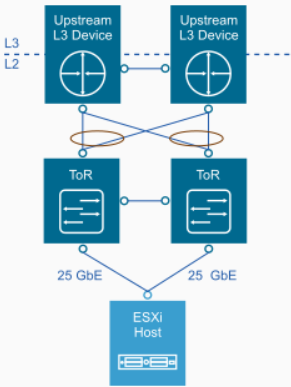
\includegraphics[width=0.3\textwidth]{imaxes/conceptosPrevios/transportlayer2.png}
%   \caption{Límite de las capas 2 y 3 cuando la topología se implementa con dispositivos de capa 2.}
%   \label{fig:transportlayer2}
% \end{figure}
% \FloatBarrier
% \begin{figure}[h!]
%   \centering
%   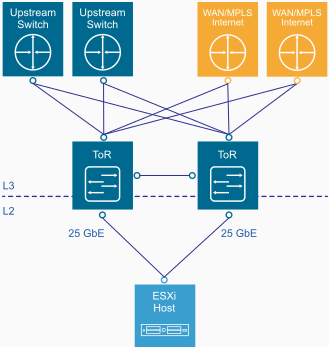
\includegraphics[width=0.3\textwidth]{imaxes/conceptosPrevios/transportNetLayer3.png}
%   \caption{Límite de las capas 2 y 3 cuando la topología se implementa con dispositivos de capa 3.}
%   \label{fig:transportlayer3}
% \end{figure}
% \FloatBarrier



% Como VMware Cloud Foundation abstrae la red física en una red virtual, la red física debe cumplir ciertos requisitos para que la red virtualizada sea robusta. Esta se debe mantener simple con configuraciones comunes en todos los switches, uso de VLANs y uso de enrutamiento dinámico, también debe ser escalable en cuanto a cantidad de hosts, ancho de banda y cantidad de rutas redundantes. Además, se debe tener en cuenta que cada tipo de tráfico tiene características diferentes, como por ejemplo el tráfico dedicado al almacenamiento a través de IP que suele usar mayor ancho de banda, por ello es necesario distinguir cada tipo de tráfico con protocolos \textit{Quality of Service} (QoS). El marcado de cada tipo de tráfico se realiza en el hipervisor ESXi a través de un vSphere Distributed Switch que soporta QoS tanto en la capa 2 como en la capa 3. En la capa 2 se utiliza  un campo de tres bits llamado \textit{Class of Service} que representa la prioridad del \textit{frame} con un valor de cero a siete, presente en la cabecera Ethernet cuando se utiliza etiquetado VLAN, mientras que en la capa 3 se utiliza un campo de 6 bits en la cabecera IP llamado \textit{Differentiated Services Code Point}, perteneciente al protocolo \textit{DiffServ}, para clasificar cada paquete. Los \underline{principales componentes que se deben configurar} para dar conectividad entre los servidores son los siguientes:
% \begin{itemize}
%     \item \textbf{Top of Rack Physical Switches} (TOR): es un switch al que se conectan los hosts de un rack para tener conectividad con el resto de la infraestructura. Se recomienda que un host esté conectado a dos switches TOR y que estos se configuren de forma redundante para proveer alta disponibilidad y tolerancia a fallos de alguna de las conexiones. Cada switch TOR se conecta a otro par de switches que establece conexión entre todos los racks.
    
%     Los puertos del switch TOR que se conectan a los hosts deben estar configurados como puertos troncales de VLAN para que acepte todas las VLANs usadas por el host, se debe proveer servicio DHCP a cada VLAN usada y configurar los puertos para que acepten \textit{jumbo frames}. El marcado QoS del tráfico que realiza cada host ESXi debe ser aceptado y no puede ser modificado una vez abandona el host. 
%     % \iffalse Además, se deben configurar todas las VLANs y subredes que se utilizarán en la infraestructura de VMware Cloud Foundation.\fi  
    
%     \underline{Otros protocolos que se deben configurar} en los puertos que se conectan con los hosts son:
%     \begin{itemize}
%         \item \emph{Spanning Tree Protocol} (STP): protocolo que se encarga de gestionar las rutas de la red que son redundantes.
%         \item \emph{Trunking}: configurar cada enlace troncal con las VLANs que van a transmitir tráfico a través de él. Se debe establecer como VLAN nativa, aquella utilizada para transmitir el tráfico que no tiene etiqueta, VLAN de la red \textit{management}.
%         \item \emph{MTU}: configurar el MTU de cada VLAN para el transporte de paquetes \textit{jumbo frames}. Este valor será el que se use para configurar los hosts ESXi. Se recomienda establecerlo en 9000 bytes.
%         \item \emph{Multicast}: configurar el protocolo IGMP en cada switch TOR como enrutador (busca activamente que VLANs pertenecen a un grupo Multicast) y cada VLAN como miembros de IGMP (los hosts que forman parte del grupo indican su pertenencia a un grupo multicast de forma activa).
%     \end{itemize}
    

    
%     % \iffalse
%     % \item \textbf{Conectividad entre Regiones}: 
%     % \item \textbf{Conectividad entre Zonas de dispobilidad}:
%     % \fi
% \end{itemize}

% Los siguientes servicios usados por los componentes de VMware Cloud Foundation se deben configurar sobre la red física de la infraestructura para el correcto funcionamiento del SDDC\cite{CFexternalServices}:
% \begin{itemize}
%     \item \textbf{Servidor DNS}: se utiliza para obtener los nombres y direcciones de todas las máquinas virtuales que se creen, tanto en sentido \textit{fordward} (obtener una dirección IP a partir de un nombre) como en sentido \textit{reverse} (obtener un nombre a partir de una dirección IP). Además, este servicio debe ser configurado antes de realizar el despliegue de VMware Cloud Foundation. Este servicio es utilizado por el componente Platform Services Controller, vCenter Server, NSX Manager y vRealize Log Insight.
    
%     \item \textbf{Servidor DHCP}: permite asignar direcciones IP de forma dinámica a los puertos \textit{vmkernel} de cada host ESXi. Este debe ser accesible desde cada VXLAN de VMware NSX y es necesario establecer previamente las redes que se van a usar en VMware Cloud Foundation. Este servicio debe estar disponible antes de comenzar el despliegue del SDDC ya que es necesaria la asignación dinámica de IPs.
    
%     \item \textbf{Servidor NTP}: requerido por todos los componentes de VMware Cloud Foundation para mantener sus horas sincronizadas. Este servicio debe estar disponible en la infraestructura y configurado en cada host ESXi antes del despliegue de VMware Cloud Foundation, y debe ser alcanzable desde la red de \textit{management} y de vRealize. La derencia de tiempo entre los componentes de la infraestructura no debe ser mayor de cinco minutos.
    
%     \item \textbf{Router}: debe existir enrutamiento dinámico en la red desde la capa 3. Es requerido por NSX para establecer comunicación con los ESG. Este servicio debe estar configurado antes del comenzar enl despliegue de VMware Cloud Foundation. 
% \end{itemize}

% \end{subsubsection}


% \begin{subsubsection}{Host ESXi\cite{WDminRequierements}}
% Los hosts ESXi que se desplieguen en un cluster deben tener características físicas idénticas para hacer la infraestructura más manejable,  incluyendo la configuración de almacenamiento y red. Para desplegar VMware Cloud Foundation se requiere:
% \begin{itemize}
%     \item  Dos interfaces de red (NIC) de la misma velocidad que deben estar conectadas a la VLAN troncal de dos switches TOR. Configurando \textit{NIC teaming} en VMware Sphere Distributed Switch se consigue que el tráfico se distribuya por las interfaces de red disponibles de forma óptima y que exista tolerancia a fallos.
%     \item Todas las conexiones físicas del host deben tener al menos una velocidad igual a 10 Gbit.
%     \item Cada host debe tener al menos 192 GB de memoria RAM, de esa cantidad, 176 GB de memoria RAM son requeridos por las máquinas virtuales que gestionan el SDDC.
%     \item Un disco de arranque con un tamaño mínimo de 16 GB.
% \end{itemize}

% \end{subsubsection}


% \begin{subsubsection}{Almacenamiento físico}
% VMware Cloud Foundation utiliza VMware vSAN para proveer el almacenamiento de un SDDC. Para desplegar VMware Cloud Foundation, VMware vSAN requiere las siguientes características:
% \begin{itemize}
%     \item Mínimo de tres hosts con recursos de almacenamiento.
%     \item Determinar qué configuración de vSAN se va a utilizar, \textit{All-Flash} o \textit{Hybrid}. Se recomienda la solución \textit{All-Flash} ya que ofrece mayor rendimiento.
%     \item Para cada host con recursos de almacenamiento se debe cumplir que el disco de caché tenga un 10\% de la capacidad del almacenamiento persistente del grupo de discos, tener un mínimo de dos discos en la capa de capacidad, un controlador RAID y configurar habilitar vSphere High Availability  para apagar las máquinas virtuales de un host cuando este se encuentre aislado. El controlador RAID debe tener la característica \textit{pass-through} la cual permite que VMware vSAN muestre como discos individuales cada disco duro de un grupo de discos, esto facilita la gestión de cada disco y que se puedan realizar sustituciones sin detener el servicio.
%     \item La capacidad mínima de almacenamiento disponible para el modelo consolidado es de 800 GB. 
% \end{itemize}

% \end{subsubsection}

% \end{subsection}

\begin{section}{Prueba de concepto}
    \label{subsect:prueba-concepto}
Para no afectar al funcionamiento de los trabajos que se llevan a cabo en el CITIC, el proyecto se lleva a cabo en un entorno aislado formado por un host y un datastore, en el cual se despliegan todos los componentes de VCF con el fin mostrar y probar las capacidades y características de VMware Cloud Foundation. 
El proceso se realizará siguiendo la metodología Scrum, donde en cada ciclo se realiza el despliegue de uno o varios componentes y posteriormente se revisa su configuración y funcionamiento. Primero se instalarán los componentes base de VMware Cloud Foundation\footnote{Los componentes base de VCF son VMware vSphere, VMware vSAN y VMware NSX-T} usando el programa VMware Lab Constructor (VLC) v4.0.1\footnote{Herramienta que permite crear un generar de forma automatizada un entorno embebido para probar las funcionalidades de VMware Cloud Foundation.}. Después se instalarán los componentes de la suite VMware vRealize, uno dedicado a la gestión de usuarios del SDDC, otro que proporciona un servicio de aprovisionamiento de recursos y otro que se encarga de la medición de los recursos. Finalmente, se comprobará el funcionamiento general del SDDC y las posibilidades que ofrece el servicio Cloud desplegado.

\begin{subsection}{Preparación}
  En esta sección se describe como se prepara el entorno de pruebas con los elementos y servicios utilizados para realizar el despliegue de la solución y necesarios para su correcto funcionamiento.

  \begin{subsubsection}{VMware Lab Constructor v4.0.1}
    El programa VMware Lab Constructor v4.0.1 (VLC), es una herramienta desarrollada por trabajadores de VMware, la cual permite crear un entorno embebido dentro del host utilizado como entorno de pruebas. Este entorno se compone de cuatro hosts con el hipervisor ESXi en forma de VMs. Dentro de estos hosts, VLC despliega los componentes de VCF.

    \begin{figure}[h!]
      \centering
      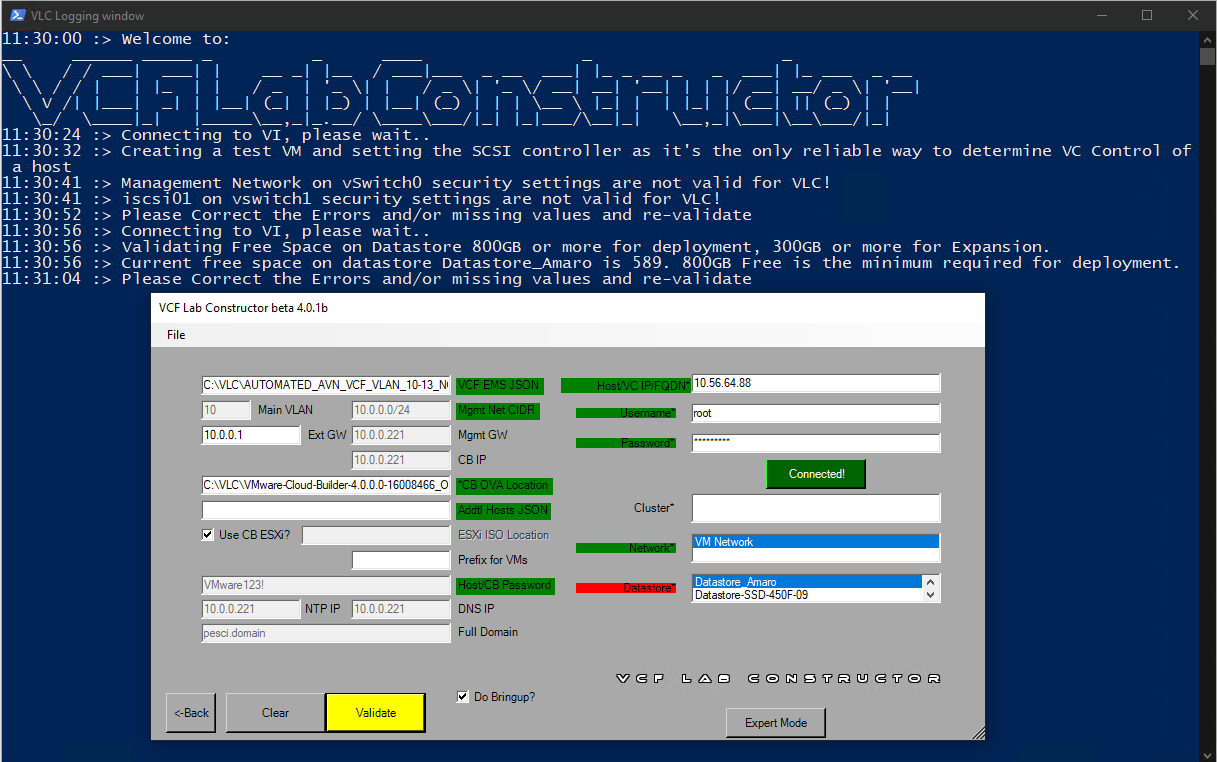
\includegraphics[width=0.8\textwidth]{imaxes/pruebaconcepto/VLC.png}
      \caption{Herramienta VMware Lab Constructor v4.0.1b}
      \label{fig:VLC}
    \end{figure}
    \FloatBarrier

  \end{subsubsection}

  \begin{subsubsection}{Host ESXi}  
    El host sobre el que VLC realiza la instalación del entorno se trata de un servidor con el hipervisor ESXi instalado. Este servidor cuenta con una memoria RAM de 192 GB, una CPU de 28,8 GHz y está conectado a un datastore formado por discos SSD y con una capacidad de 3 TB. Además, incorpora dos interfaces de red. La primera interfaz se conecta a una red para acceder al datastore, mientras que la segunda, representada con el nombre \textit{vmnic0} en la figura \ref{fig:estructura-generada-por-VLC}, se conecta a una red utilizada para acceder de forma remota al servidor y a otra red dedicada a comunicar los componentes desplegados dentro del host.

    % Como base para la instalación se utiliza un servidor físico con el hipervisor ESXi instalado. Este host se utiliza para desplegar los componentes de VMware Cloud Foundation para crear un pequeño SDDC embebido para probar sus funciones. Este host cuenta con una memoria RAM de 192 GB, una CPU de 28,8 GHz y un \textit{datastore} con discos SSD con 2 TB de capacidad. Cuenta con dos interfaces físicas, una que conecta al host con el \textit{datastore} y otra a la que se conectan dos redes, una llamada \textit{Management Network} que permite acceder al host desde una VM para gestionarlo, y otra llamada \textit{VM Network} donde se conectan todas las VMs generadas por VLC y de los servicios que dan soporte a los componentes de VMware Cloud Foundation.
  \end{subsubsection}

  \begin{subsubsection}{Servicios}
    Los servicios externos requeridos por VCF se sitúan dentro del mismo servidor físico. Estos están colocados en una VM con el sistema operativo Windows Server 2016, el cual incluye DNS, NTP, SMTP, y los servicios Active Directory (AD) y Certificate Authority (CA). También incorpora un router en forma de VM con el sistema operativo VyOS, que además cuenta con servicio DHCP. El servidor DNS utiliza \textit{pesci.domain} como nombre de dominio. El almacén Active Directory sustituye al directorio de usuarios de la UDC para poder manejar cuentas de usuarios sin causar conflictos en el funcionamiento de los servicios en producción.
    % Todos los servicios requeridos por VMware Cloud Foundation se despliegan sobre el mismo servidor en forma de VMs. Una de las VMs es Windows Server 2016 que contiene un servidor DNS, un servidor NTP, un servidor Active Directory, un servidor SMTP y ejerce también como Certificate Authority. Otra VM contiene el sistema operativo VyOS que funciona como un router virtual y como servidor DHCP. Una última VM con Windows 10\footnote{Se refiere a ella como \textit{Jump Host}.} se requiere para ejecutar VLC y acceder al entorno embebido generado por VLC.
    % El servidor DNS contiene el nombre y su respectiva dirección que un componente de VCF utilizará para que sus instancias se puedan comunicar con otras. Este servidor DNS implementa un único dominio que se denomina \textit{pesci.domain}. El servidor Active Directory proporciona un almacén de usuarios y grupos de usuarios a los cuales se les configura un rol dentro de cada componente de SDDC. Se utiliza este repositorio de usuarios en lugar del directorio real de la UDC para evitar posibles problemas del servicio. El router VyOS tiene configuradas todas las subredes y VLANs que VMware Cloud Foundation utiliza en la capa L3 de la infraestructura física y proporciona acceso a Internet, en las cuatro interfaces que conectan con las instancias de VMware NSX-T Edge utiliza enrutamiento dinámico BGP. El servidor DHCP se utiliza para asignar una dirección IP a las interfaces Tunnel EndPoint (TEP)\footnote{Más adelante se describirá la función de este elemento} de cada host ESXi.    
  \end{subsubsection}
  \begin{figure}[h!]
    \centering
    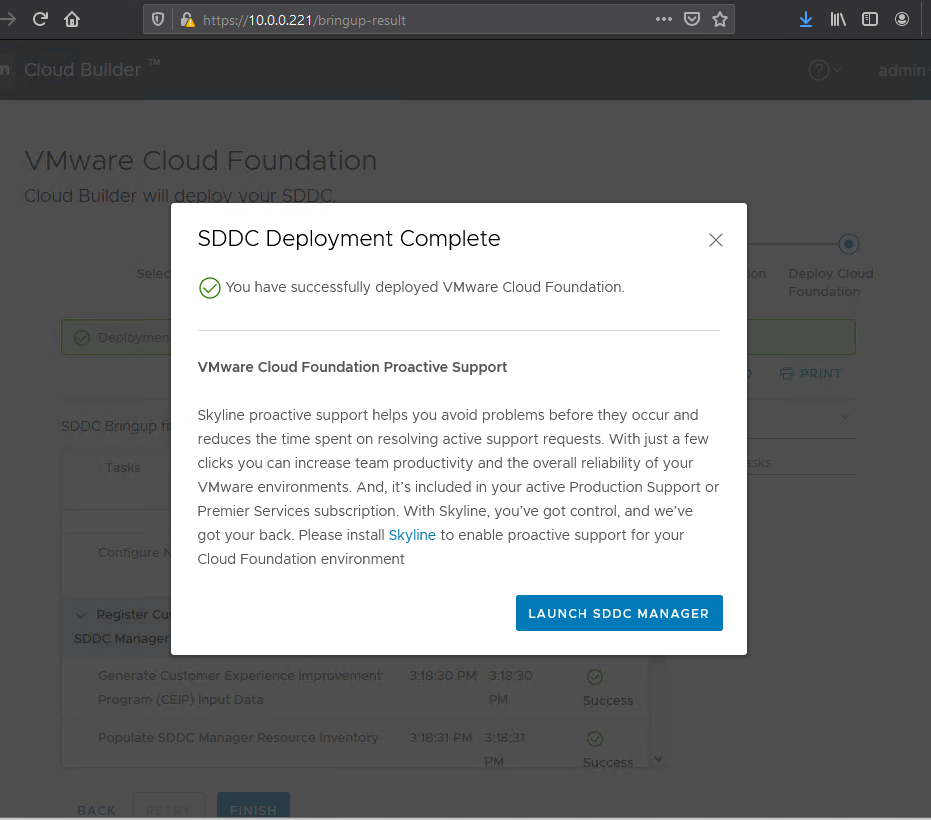
\includegraphics[width=0.7\textwidth]{imaxes/pruebaconcepto/fin-despliegue.png}
    \caption{Finalización del despliegue inicial de VMware Cloud Foundation.}
    \label{fig:fin-despliegue}
  \end{figure}
  \FloatBarrier
    \begin{figure}[h!]
      \centering
      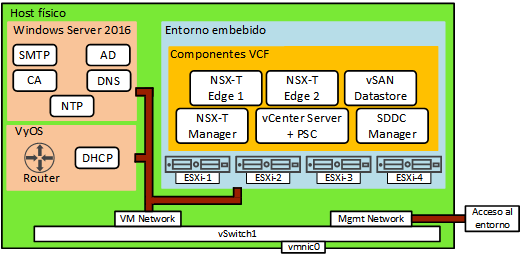
\includegraphics[width=0.8\textwidth]{imaxes/pruebaconcepto/hostFisico.png}
      \caption{Servicios desplegados y entorno embebido generado por VLC dentro del host físico.}
      \label{fig:estructura-generada-por-VLC}
    \end{figure}
    \FloatBarrier
    Una vez finalizado el despliegue como se muestra en la figura \ref{fig:fin-despliegue}, el entorno embebido generado con VLC dentro del host físico, incluyendo las VMs de los componentes de VCF y los servicios necesarios para su correcto funcionamiento, se muestra en la figura \ref{fig:estructura-generada-por-VLC}. Esta figura también incluye las dos redes a las que se conecta la interfaz \textit{vmnic0} del host. \textit{VM Network} comunica a todos los elementos desplegados y representa la red física del entorno. La red \textit{Mgmt Network} se utiliza para acceder al host de forma remota.
    % \begin{figure}[h]
    %   \centering
    %   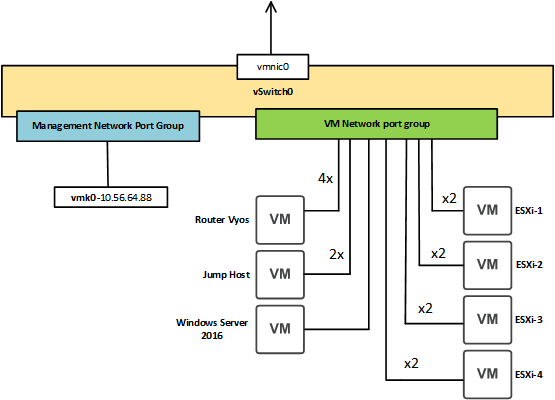
\includegraphics[width=0.6\textwidth]{imaxes/pruebaconcepto/vSwitch0HostFisico.png}
    %   \caption{Máquinas virtuales en el host físico.}
    %   \label{fig:VMs-alojadas-host-fisico}
    % \end{figure}
    % \FloatBarrier

    % En la imagen anterior se muestran las VMs que están funcionando sobre el host físico y que representan los componentes de la infraestructura física de un SDDC real, junto con el número de interfaces que se utilizan en cada una. Cada host ESXi generado por VLC cuenta con dos interfaces de red. El router VyOS, Jump Host y Windows Server 2016 se configuran antes del despliegue de VMware Cloud Foundation con VLC y se comunican con el entorno generado por VLC a través del \textit{port group} VM Network. El \textit{port group} Management Network se utiliza para acceder a la configuración del host físico a través de la dirección IP que se indica. Se utiliza la interfaz vmnic0 del host como salida del tráfico generado por el vSwitch0.
    % \FloatBarrier

    % \begin{figure}[h]
    %   \centering
    %   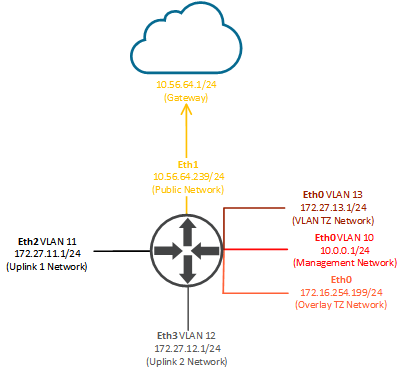
\includegraphics[width=0.4\textwidth]{imaxes/pruebaconcepto/RouterFisicoL3.png}
    %   \caption{Interfaces del router Vyos.}
    %   \label{fig:interfaces-router-fisico-L3}
    % \end{figure}
    % \FloatBarrier

    % En la imagen anterior se muestra la configuración del router VyOS. Cada una de las interfaces se debe configurar antes del despliegue de VCF. Todas usan MTU de 9000 Bytes ya que la mayoría de componentes de VCF utilizan paquetes de red \textit{jumbo frame}. En las interfaces Eth2 y Eth3 el router utiliza enrutamiento dinámico BGP donde el AS local es 65001 y el AS remoto es AS 65003, configurado para anunciar a sus vecinos la red 10.0.0.0/24 Management Network. Las direcciones configuradas como \textit{neighbour} son: 172.27.11.2, 172.27.11.3, 172.27.12.2 y 172.27.12.3. En la dirección IP 172.27.254.199 de la interfaz eth0, el router proporciona un servidor DHCP que asigna direcciones IP en el rango 172.16.254.0 - 172.16.254.100.
    % \FloatBarrier

    % \begin{figure}[h]
    %   \centering
    %   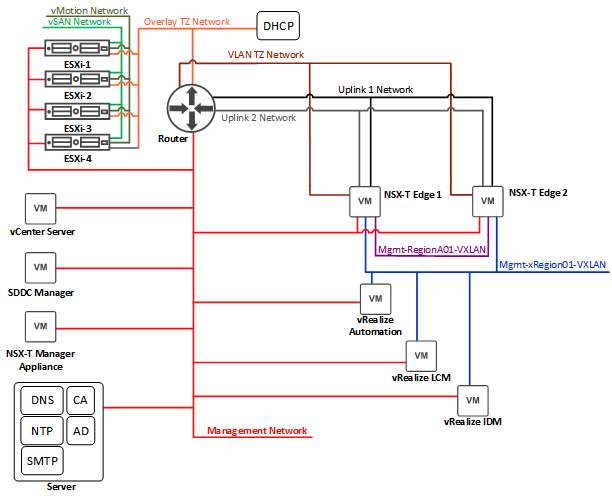
\includegraphics[width=0.6\textwidth]{imaxes/pruebaconcepto/RedDesdeDentro.png}
    %   \caption{Topología de las redes del entorno desplegado.}
    %   \label{fig:red-L3-infraestructura-fisica}
    % \end{figure}
    % \FloatBarrier

    % En la imagen anterior se muestran todos los componentes de VMware Cloud Foundation desplegados por VLC y los desplegados posteriormente para completar los objetivos del proyecto, como se conectan con los distintos servicios de red y a que redes se conectan. Las redes Mgmt-xRegion01-VXLAN y Mgmt-Region01A-VXLAN se corresponden a redes virtuales gestionadas por VMware NSX-T que no requieren ninguna configuración adicional en la capa 3 de la infraestructura física (esto se verá con detalle en el apartado de diseño de VMWare NSX-T).
    % \FloatBarrier
  \end{subsection}

\begin{subsection}{Diseño y configuración del Management Domain}
\input{contido/metodoloxia/pruebaconcepto/diseñovSphere}
\input{contido/metodoloxia/pruebaconcepto/diseñoNSX-T}
\end{subsection}
\begin{subsection}{Operaciones de la Arquitectura}
    En este punto ya se ha formado el SDDC, la configuración de la infraestructura física y de todos sus componentes está lista para desplegar los componentes que habiliten el servicio Cloud de aprovisionamiento de recursos. Este último paso se completará con los productos agrupados bajo VMware vRealize Suite. Se utilizarán tres de estos productos, vRealize Operations Manager(vROps), Workspace One Access (WSA) y vRealize Automation (vRA).
    % En este punto ya se ha formado el SDDC, la configuración de la infraestructura física y de todos sus componentes está lista para desplegar los componentes que habiliten el servicio Cloud de aprovisionamiento de recursos. Este último paso se completará con los productos agrupados bajo VMware vRealize Suite. Se utilizarán tres des estos productos, vRealize Suite Lifecycle Manager (vRSLCM), Workspace One Access (WSA) y vRealize Automation (vRA).
    %  y, para aprovechar las ventajas de VMware NSX-T y las redes virtuales existentes, utilizarán como red de acceso el Segment \textit{mgmt-xRegion01-VXLAN}.
    % estos proporcionarán un servicio de autenticación centralizado para los usuarios y servicio de aprovisionamiento de recursos
    % El entorno ya está configurado para funcionar como un SDDC, a partir de este punto ya no es necesario realizar ninguna modificación en la infraestructura física ya que todas las tareas que se deben realizar están dentro del alcance de los componentes de VMware Cloud Foundation. Para finalizar la construcción del SDDC y habilitar un servicio donde los usuarios puedan aprovisionar recursos bajo demanda, se instalarán sobre el entorno desplegado las aplicaciones Workspace ONE Access \footnote{VMware vRealize Identity Manager} (WSA) y VMware vRealize Automation (vRA). La primera permite al administrador conectar con el servidor de usuarios Active Directory y gestionarlos para proveer un servicio de autenticación centralizado a múltiples aplicaciones como VMware vRealize Automation. La segunda aplicación permite a los usuarios aprovisionar recursos de forma automatizada desde un catálogo de recursos. VMware vRealize Suite Licfecycle Manager (vRSLCM) es el componente que permite administrar vRA y WSA, su instalación y actualizaciones, las contraseñas de administrador y sus certificados, para ello necesita comunicarse con VMware vCenter Server. Se desplegará una instancia de cada componente en el \textit{management domain} creado anteriormente y estarán conectadas al \textit{segment}/subred \textit{Mgmt-xRegion01-VXLAN}.
    % \begin{subsubsection}{vRealize Operations Manager}
    %     vROps se instala en el entorno para establecer un sistema de valoración de los recursos. Gracias a este componente, el administrador del SDDC será capaz de establecer una valoración de los recursos consumidos por los usuarios con el fin de establecer un límite de consumo total para cada usuario. Además, también permitirá al administrador del SDDC acceder a estadísticas y eventos donde vROps analiza información obtenida de la infraestructura para detectar problemas, proponer soluciones y monitorizar el uso de recursos. vROps monitoriza y obtiene métricas de los recursos disponibles en VMware vCenter Server, VMware NSX-T y VMware vSAN para recopilar los eventos e información de cada uno de ellos con el objetivo de predecir posibles problemas y automatizar la aplicación de soluciones. Además, se integra con vRealize Automation para mostrar al usuario en su portal de acceso información sobre los recursos que utiliza.
    %     \\
    %     \begin{figure}[h]
    %         \centering
    %         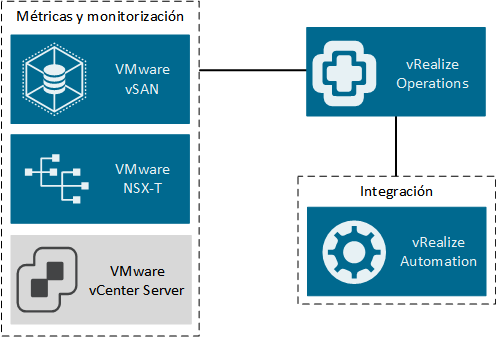
\includegraphics[width=0.4\textwidth]{imaxes/pruebaconcepto/vrealize/estructura-vrops.png}
    %         \caption{Componentes con los que se comunica vROps.}
    %         \label{fig:vrops-components}
    %     \end{figure}
    %     \FloatBarrier
    %     El sistema de valoración que se puede habilitar con vROps consiste en que se establecen una serie precios en una divisa determinada. Por el uso de CPU, memoria RAM y almacenamiento se establece un precio y a medida que los usuarios utilicen el servicio Cloud, vROps se encargará de calcular el precio total de los recursos que ha consumido cada usuario durante un periodo e tiempo. De esta forma el administrador puede obtener una métrica de cuantos ha consumido un usuario y, en caso de que supere un límite establecido poder actuar en consecuencia reduciendo la cantidad de recursos disponibles para el usuario o no permitirle su uso temporalmente.
        % vRSLCM es el primer componente que se instala ya que es el encargado de gestionar el ciclo de vida de los productos de VMware vRealize Suite, incluyendo su despliegue, actualizaciones y gestión de las credenciales de administración, certificados y licencias, por lo tanto permite al administrador del SDDC controlar de forma centralizada la configuración y seguridad de los servicios dedicados a las operaciones del SDDC. Para llevar a cabo sus funciones, vRSLCM debe comunicarse con la instancia de VMware vCenter Server desplegada en el Management Domain.
        % vRSLCM es el primer componente que se instala ya que es el encargado de gestionar el ciclo de vida de los productos de VMware vRealize Suite, incluyendo su despliegue, actualizaciones y gestión de las credenciales de administración, certificados y licencias, por lo tanto permite al administrador del SDDC controlar de forma centralizada la configuración y seguridad de los servicios dedicados a las operaciones del SDDC. Para llevar a cabo sus funciones, vRSLCM debe comunicarse con la instancia de VMware vCenter Server desplegada en el Management Domain.
        % este componente está dedicado a mantener su seguridad y configuración, y a controlar que servicios se encuentran en el entorno, todo para simplificar y facilitar las tareas del administrador. Para llevar a cabo sus funciones, vRSLCM debe mantener una comunicación con la instancia de VMware vCenter Server desplegada en el Management Domain.
        % \begin{figure}[h]
        %     \centering
        %     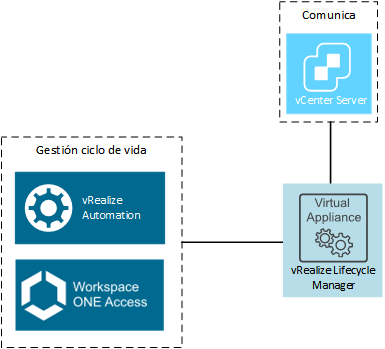
\includegraphics[width=0.4\textwidth]{imaxes/pruebaconcepto/vrealize/diseno-vrlscm.png}
        %     \caption{Componentes con los que se comunica vRSLCM.}
        %     \label{fig:vrealize-components}
        % \end{figure}
        % \FloatBarrier        
        % Durante el despliegue de WSA y vRA, desde vRSLCM se establece su configuración, indicando la licencia, credenciales del administrador, direcciones IP, configuración DNS y NTP, y certificados\footnote{El certificado de cada aplicación es generado manualmente desde la CA y luego subido a vRSLCM, que en este caso es la VM con Windows Server 2016.} para habilitar el acceso seguro desde el navegador web. Las instancias de cada componente desplegado se colocan dentro del cluster vSphere\footnote{\nameref{subsubsec:diseno-vsphere}} creado anteriormente, y utilizarán uno de los Segments creados en VMware NSX-T para conectarse a la red\footnote{Figura \ref{fig:two-tier-topology}}.
% Además, se debe elegir la ubicación donde se van a desplegar las VMs de estos servicios, es decir, el dominio de VMware vCenter Server, el cluster vSphere, la red y el datastore para el almacenamiento.
        
        % En el entorno de pruebas, de cada servicio se crea una instancia en el Management Domain. Cada una se coloca en el cluster vSphere (\nameref{subsubsec:diseno-vsphere}), utilizan el datastore de VMware vSAN (\nameref{subsubsec:diseno-vsan}) y están controladas por la instancia de VMware vCenter Server (\nameref{subsubsec:diseno-vcenter}). Como ya se ha mencionado, las instancias se conectan a un Segment controlado por VMware NSX-T (como se muestra en la figura \ref{fig:two-tier-topology}) para poder hacer uso de sus servicios de red.
        % \begin{figure}[h]
        %     \centering
        %     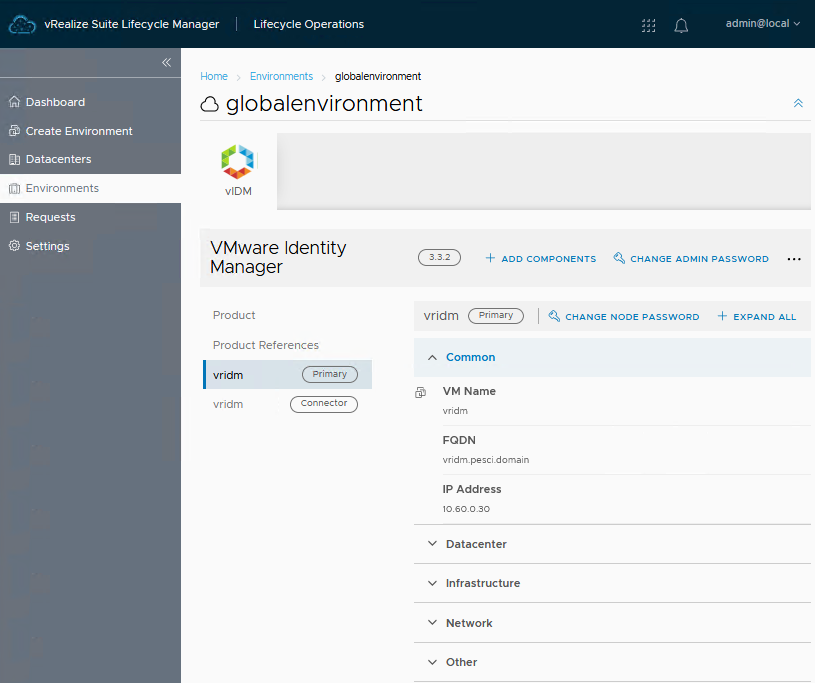
\includegraphics[width=0.6\textwidth]{imaxes/pruebaconcepto/vrealize/config-istance-vridm.png}
        %     \caption{Apartado donde se muestra la configuración de la instancia de WSA en vRSLCM.}
        %     \label{fig:config-WSA}
        % \end{figure}
        % \FloatBarrier
        
        % Dentro de vRSLCM, los despliegues son organizados por entornos pudiendo crearse un entorno por cada servicio o un entorno con todos los servicios. Existen dos modos de despliegue, uno donde se crean tres instancias del servicio para balancear la carga\footnote{El balanceo de la carga se realiza con el servicio de Load Balancing de VMware NSX-T.}, y otro donde solo se crea una instancia.

        % En el entorno, se despliega una instancia de cada servicio. Estas están colocadas bajo el dominio de la instancia de VMware vCenter en el cluster vSphere

        % Este se instala desde SDDC Manager, pero una vez instalado es utilizado para desplegar cualquier servicio de VMware vRealize Suite.
    % \end{subsubsection}
    \begin{subsubsection}{Workspace One Access}
        \label{subsubsec:WSA}
        WSA permite integrar un directorio de usuarios para proporcionarles acceso al servicio Cloud. Así, en el entorno real del CITIC, WSA estaría integrado con el directorio de usuarios de la UDC para que estos pudieran acceder al servicio de aprovisionamiento utilizando las credenciales de la UDC.\\
        En el entorno de pruebas, WSA está integrado con el directorio de usuarios Active Directory situado en la VM con Windows Server 2016. Este Active Directory contiene perfiles de usuarios y grupos de usuarios organizados en unidades organizativas. Los perfiles de usuario se añaden a grupos de usuarios y la creación y mantenimiento de sus credenciales se realiza desde el propio Active Directory. Desde WSA se seleccionan los usuarios y grupos de usuarios que se quieren sincronizar, para habilitarlos dentro del SDDC y posteriormente configurar su acceso al servicio Cloud. Como norma general, los permisos y roles se deben aplicar sobre grupos de usuarios y no a perfiles individuales, de esta forma se reduce el tiempo de gestión y se simplifica la estructura del directorio ya que se configura el acceso de un conjunto de usuarios al mismo tiempo.\\
        Los usuarios configurados en el Active Directory son sincronizados en WSA y serán utilizados para mostrar las funcionalidades del servicio Cloud como si se tratase del entorno en producción. Para realizar la sincronización se seleccionarán las unidades organizativas necesarias.
        % , ya que para asignar nuevos permisos a un usuario solo sería necesario añadirlo al grupo correspondiente.        
        % En el Active Directory se han configurado varios usuarios que se sincronizan en WSA. Estos se utilizarán para mostrar las funcionalidades de vRA como si se tratase del entorno real con perfiles de usuarios de la UDC.
        
        \begin{figure}[h]
            \centering
            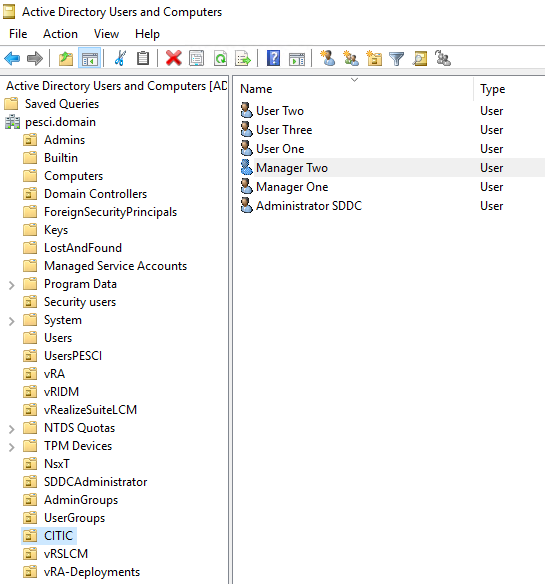
\includegraphics[width=0.6\textwidth]{imaxes/pruebaconcepto/vrealize/UnidadesOrg-Users-AD.png}
            \caption{Unidades organizativas configuradas en el AD junto a los usuarios pertenecientes a la unidad CITIC.}
            \label{fig:users-defined-AD}
        \end{figure}
        \FloatBarrier
        % En WSA se seleccionan aquellas unidades organizativas que se quieren sincronizar. Cada unidad contiene usuarios y grupos de usuarios, los usuarios que harán uso del servicio de aprovisionamiento están colocados en la unidad CITIC.
        \begin{figure}[h]
            \centering
            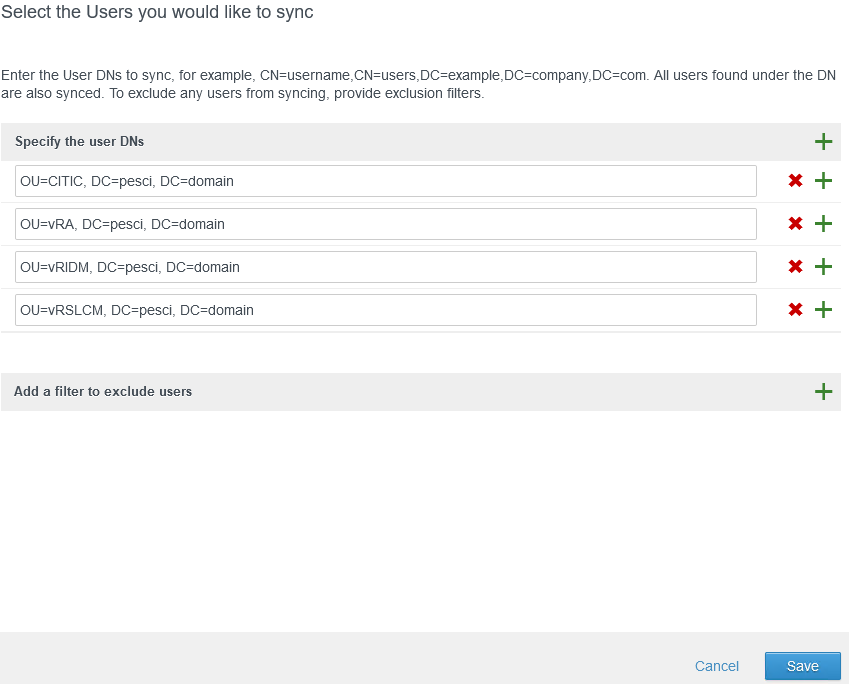
\includegraphics[width=0.6\textwidth]{imaxes/pruebaconcepto/vrealize/syncing-users.png}
            \caption{Sincronización de usuarios desde Workspace One Access seleccionando Unidades Organizativas.}
            \label{fig:users-defined-WSA}
        \end{figure}
        \FloatBarrier
        \begin{figure}[h]
            \centering
            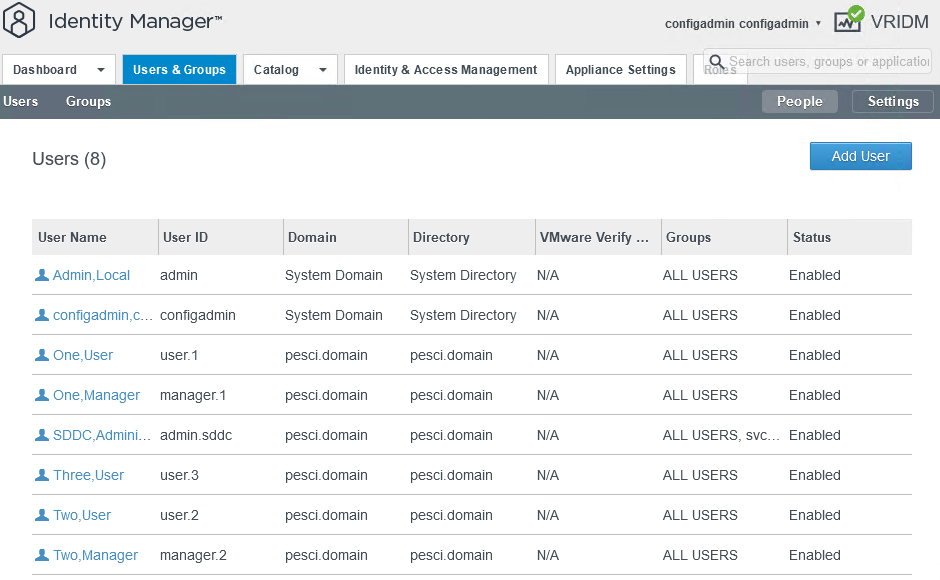
\includegraphics[width=0.6\textwidth]{imaxes/pruebaconcepto/vrealize/users-wsa.png}
            \caption{Usuarios sincronizados en Workspace One Access.}
            \label{fig:users-defined-WSA}
        \end{figure}
        \FloatBarrier
        El acceso al servicio Cloud está centralizado a través de una plataforma de autenticación proporcionada por WSA. Cuando el usuario intenta acceder al servicio este es redirigido a una página web donde introduce sus credenciales, WSA comprueba los datos introducidos y vuelve a redirigir al usuario a la pantalla del servicio. Utilizando esta plataforma  de autenticación el administrador del SDDC puede obtener estadísticas sobre qué usuarios se autentican, a qué servicios acceden y desde dónde lo hacen. Además, también se pueden  modificar los parámetros de autenticación y la configuración las sesiones de usuarios, permitiendo definir si el usuario debe utilizar su cuenta de correo electrónico o nombre de usuario para iniciar sesión o si se utilizan cookies de sesión o persistentes. Por si esto fuera poco, también existe la posibilidad de crear políticas para controlar desde dónde pueden los usuarios acceder al servicio y el tiempo de duración de las sesiones. En la siguiente figura se muestran las reglas de la política por defecto que se aplica, en esta se permite el acceso desde cualquier dirección IP, a través de un navegador web, usando su contraseña y con un tiempo de sesión de 8 horas.
        \begin{figure}[h]
            \centering
            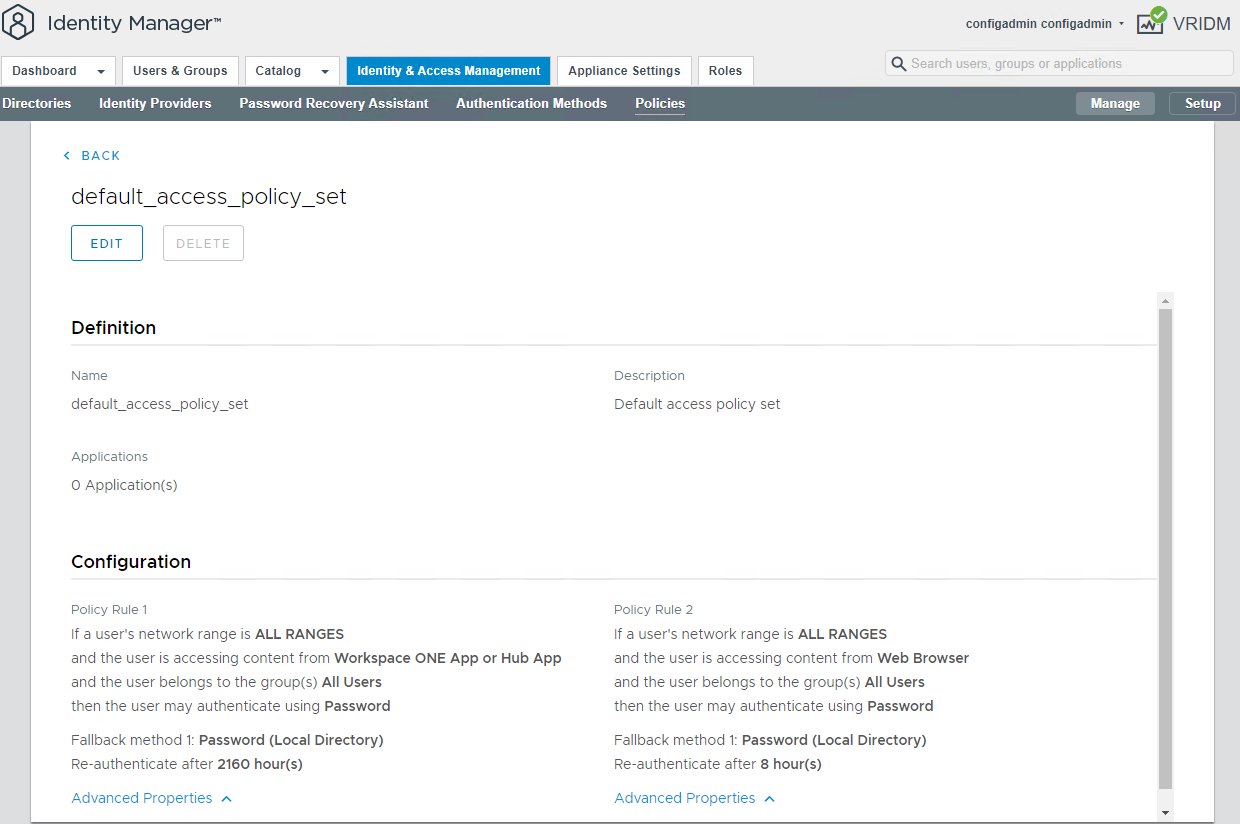
\includegraphics[width=0.6\textwidth]{imaxes/pruebaconcepto/vrealize/default-policy.png}
            \caption{Política de autenticación por defecto establecida en WSA.}
            \label{fig:default-policy}
        \end{figure}
        \FloatBarrier
        \begin{figure}[h]
            \centering
            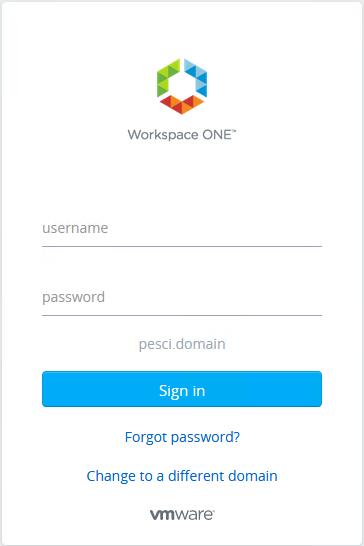
\includegraphics[width=0.3\textwidth]{imaxes/pruebaconcepto/vrealize/wsa-login.png}
            \caption{Plataforma de autenticación de Workspace One Access.}
            \label{fig:wsa-platform}
        \end{figure}
        \FloatBarrier        
        Con WSA el administrador tiene un mayor control sobre los usuarios y cómo estos acceden al servicio Cloud, ya que desde un único punto se gestionan todos los perfiles de usuarios disponibles y la seguridad de acceso, pudiendo controlar qué usuarios acceden y establecer medidas seguridad de forma sencilla. La gestión de las credenciales de cada usuario se separa de la gestión del acceso, ya que lo primero está controlado por el AD y lo segundo por WSA. De esta forma la seguridad del entorno aumenta y las tareas del administrador se simplifican. Con esta plataforma se soluciona uno de los problemas de la infraestructura del CITIC, ya no es necesario crear un perfil manualmente para cada usuario que quiera acceder al servicio y su gestión se centraliza en un componente dedicado a ello.

        % Los usuarios que necesiten acceder a vRA deben estar registrados en el directorio de Workspace One Access. Este componente centraliza el acceso de todos los productos de VMware vRealize. Cuando se despliega se debe configurar un Active Directory que en el caso del entorno está situado en la VM con Windows Server 2016. Dentro del Active Directory existen grupos de seguridad y perfiles de usuario, un perfil de usuario contiene información como nombre, apellidos, dirección e-mail, nombre de usuario y contraseña\footnote{Se pueden configurar más campos pero los que se describen son los obligatorios a la hora de crear un usuario.}, y este puede formar parte de varios grupos de seguridad. Una vez configurado, cada aplicación se conectará a WSA y se podrán asignar roles para los grupos de seguridad y usuarios estableciendo así un nivel de acceso. Además, cada usuario registrado tendrá disponible un catálogo de aplicaciones en el portal de WSA cuyo administrador establecerá que aplicaciones están habilitadas para cada usuario o grupo, eso sí, para que el usuario pueda acceder a ella previamente se debe establecer un rol para ese usuario dentro de la aplicación.

        %*****USUARIOS QUE HAY EN EL ENTORNO Y EL ACCESO A CADA APLICACIÓN*******%
        % \begin{figure}[h]
        %     \centering
        %     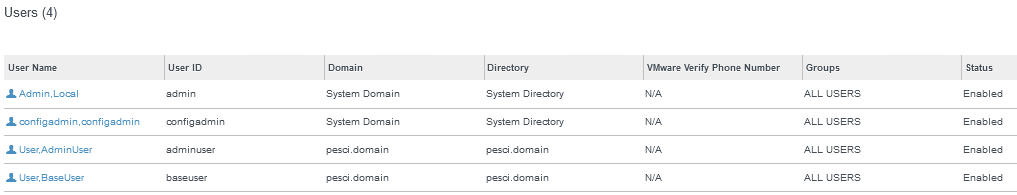
\includegraphics[width=0.4\textwidth]{imaxes/vRealize_pruebaconcepto/usuariosDefinidos.png}
        %     \caption{Muestra los usuarios definidos en el Active Directory sincronizados en Workspace One Access.}
        %     \label{fig:users-defined-AD}
        % \end{figure}
        % \FloatBarrier
        % En la Figura \ref{fig:users-defined-AD} se muestran los dos usuarios definidos en el Active Directory y dos usuarios que se corresponden a los perfiles de administración de WSA, no se utilizarán grupos de seguridad para reducir la complejidad pero su configuración en las aplicaciones de VMware es igual que para los perfiles de usuario. En un entorno real existen usuarios que controlan a otros usuarios y establecen su nivel de acceso, a parte de los perfiles de administrador de cada aplicación. Para el entorno se define el perfil \textit{adminuser} que será el encargado de gestionar el acceso de dos usuarios (\textit{baseuser1} y \textit{baseuser2}) que serán los que consuman a las aplicaciones desplegadas (vRSLCM y vRA). El primero tendrá acceso y permisos de edición en las aplicaciones vRSLCM y vRA, mientras que los dos usuarios base solo podrán acceder a vRA y dentro de este el usuario admin definirá que servicios están habilitados para cada uno.

        %************************************************************************%

    \end{subsubsection}

    \begin{subsubsection}{VMware vRealize Automation}
        VMware vRealize Automation es el componente de VMware vRealize Suite que automatiza el aprovisionamiento de recursos del SDDC. Con esta plataforma los usuarios elaboran diseños de los recursos que necesitan para posteriormente implementarlos y llevar a cabo sus trabajos. Estos diseños,son archivos con formato .yaml en los que se especifican los recursos de la infraestructura que se quieren utilizar y su configuración, como el tamaño de una VM, su sistema operativo, creación de usuarios, instalación de paquetes, redes a las que se conecta, almacenamiento que utiliza o su localización en la infraestructura. Una vez completado el diseño, el usuario lo ejecuta y vRA se encarga de aprovisionar todos los recursos especificados, de forma ordenada, automatizada y transparente. El administrador del SDDC se encargado de establecer qué recursos de la infraestructura están disponibles para los usuarios, asignando a cada uno un tag con la forma \textit{key:value} para que puedan ser referenciados.
        \\        
        Para separar el flujo de trabajo de diferentes usuarios, vRA permite la creación de proyectos que agrupan a un conjunto de usuarios, en los cuales se habilitan diseños a los que solo los miembros del proyecto tienen acceso. En cada proyecto existe el rol de administrador de proyecto y el de miembro de proyecto, el primero es el que se encarga de determinar qué usuarios tienen acceso al proyecto y de habilitar los diseños en un catálogo, el segundo solo tiene acceso a los proyectos donde ha sido admitido para aprovisionar y utilizar los recursos establecidos en los diseños disponibles. El administrador del SDDC se encarga de la creación de cada proyecto y de establecer recursos la cantidad de recursos disponibles para cada uno.
        % Durante proceso de implementación de esos diseños se aprovisionan recursos de forma automática y transparente para el usuario, que puede modificar los requisitos de sus recursos según sea necesario
        % Al mismo tiempo, el administrador establece los límites del diseño/implementación y debe proveer en la infraestructura los medios que se usarán como base para los diseños.
        % En vRA el aprovisionamiento de recursos se realiza a partir de diseños realizados por el usuario. Estos diseños, llamados Blueprints, son archivos con formato .yaml en los que se especifican los recursos que el usuario quiere obtener, estos recursos son VMs, redes y almacenamiento, y para cada recurso definido el usuario puede especificar sus características como el tamaño de una VM y su configuración interna (sistema operativo, instalación de librerías o servicios, redes a las que se conecta). Las blueprints se definen dentro de proyectos en los cuales existen jefes de proyecto y usuarios que utilizan o aprovisionan los recursos definidos en cada blueprint, de esta forma, tanto el administrador como el jefe de proyecto controlan qué usuarios acceden a los recursos de un proyecto. Además, el administrador será el encargado de limitar la cantidad de recursos disponibles para cada proyecto, y de establecer los recursos disponibles para el proyecto, es decir, qué sistemas operativos están disponibles, en qué redes se podrán realizar los despliegues y que datastore utilizarán para el almacenamiento.
        \begin{figure}[h]
            \centering
            \includegraphics[width=0.7\textwidth]{imaxes/vRealize_pruebaconcepto/ComponentesVRA.png}
            \caption{Uso y componentes de VMware vRealize Automation.}
            \label{fig:vra-components}
        \end{figure}
        \FloatBarrier
        Como se muestra en la figura anterior, en vRA existen tres componentes principales que son Service Broker, a través del cual los usuarios tienen acceso a los diseños e implementaciones de sus proyectos, Cloud Assembly, donde el administrador del SDDC establece los recursos disponibles y donde los administradores de cada proyecto se elaboran de forma automatizada los diseños, y Cloud Zone, punto desde donde vRA accede a la infraestructura para obtener los recursos.
        \\
        vRA soluciona las principales carencias de la infraestructura del CITIC y su servicio de virtualización, que son la falta de automatización en el aprovisionamiento y la falta de control sobre el uso y el acceso a los recursos. Con vRA se proporciona un servicio Cloud de tipo IaaS para la obtención de recursos de forma medida y bajo demanda, mientras el administrador del SDDC puede controlar a qué recursos accede cada usuario y cuantos recursos pueden utilizar mediante el uso del servicio de valoración proporcionado por vROps.
        % \\
        % En la siguiente sección se detallará como se han configurado los recursos de la infraestructura del entorno de pruebas en vRA y cómo son utilizados por los usuarios, ya que esta será la plataforma que complete el servicio Cloud propuesto para la infraestructura del CITIC.
        % Internamente vRA se divide en tres componentes, Cloud Assembly, Service Broker y Cloud Zone.
        % El punto a través del cual los usuarios pueden aprovisionar sus recursos es vRealize Automation. Este producto provee el servicio cloud. 
        % \begin{figure}[h]
        %     \centering
        %     \includegraphics[width=0.8\textwidth]{imaxes/vRealize_pruebaconcepto/ComponentesVRA.png}
        %     \caption{Componentes de VMware vRealize Automation y tareas que realiza cada rol de usuario.}
        %     \label{fig:vra-components}
        % \end{figure}
        % \FloatBarrier
        % Internamente vRA se divide en varios servicios que permiten gestionar los diferentes aspectos de la cloud. Para centrarse en los objetivos de este proyecto solo se hace referencia a dos de esos servicios, el primero es Cloud Assembly el cual permite administrar la infraestructura disponible controlar el uso que se hace de esos recursos, y el segundo es Service Broker, utilizado por los usuarios para aprovisionar los recursos desde un catálogo de plantillas. La obtención de los recursos por parte del usuario se hace desplegando una serie de plantillas llamadas Blueprints diseñadas previamente, en donde se define un conjunto de VMs y recursos de red y de almacenamiento incluyendo otros aspectos como la configuración de cada uno de los recursos, como redes de la infraestructura que se utilizan, cantidad de almacenamiento, o la ubicación del despliegue en la infraestructura. Son ficheros de código con extensión \textit{.yaml} donde se indican etiquetas, aunque también se pueden diseñar con un editor gráfico. Estas plantillas están relacionadas con proyectos, una plantilla pertenece a uno o varios proyectos donde existe un coordinador de proyecto que se encarga de diseñar Blueprints y de administrar los usuarios miembros de ese proyecto. Los proyectos de vRA permiten limitar los recursos para que un conjunto de usuarios pueda desplegar los componentes definidos en las Blueprints disponibles, como la cantidad de memoria RAM, cantidad de instancias que se pueden desplegar y cantidad de almacenamiento, también aquellas redes que se pueden utilizar. Desde el punto de vista de vRA, la infraestructura se divide en Cloud Zones, las cuales son conjuntos de recursos situados en distintos proveedores Cloud que pueden ser públicos como AWS o Azure, o privados que solo pueden ser clusters vSphere. En el caso del entorno desplegado solo se tendrá una única Cloud Zone de tipo vSphere. En cada Cloud Zone se define como se deben distribuir los recursos aprovisionados sobre la infraestructura. 
        % Finalmente será el administrador de la infraestructura el que se encargue de proveer los recursos, administrar los proyectos disponibles, gestionar los coordinadores de cada proyecto y controlar y limitar el uso de los recursos.
        % Finalmente, vRA permite configurar tarjetas donde se puede definir el coste del aprovisionamiento de CPU, almacenamiento y memoria RAM, además del coste de uso de otros elementos como sistemas operativos, el uso de una determinada red o el uso de una determinada Cloud Zone. Estas tarjetas se asignan por proyecto para determinar el coste que tendrá el consumo de recursos por mes.
    \end{subsubsection}
    \begin{subsubsection}{vRealize Operations Manager}
        vROps se instala en el entorno para establecer un sistema de valoración de los recursos. Gracias a este componente, el administrador del SDDC será capaz de establecer una valoración de los recursos consumidos por los usuarios con el fin de establecer un límite de consumo total para cada usuario. Además, también permitirá al administrador del SDDC acceder a estadísticas y eventos donde vROps analiza información obtenida de la infraestructura para detectar problemas, proponer soluciones y monitorizar el uso de recursos. vROps monitoriza y obtiene métricas de los recursos disponibles en VMware vCenter Server, VMware NSX-T y VMware vSAN para recopilar los eventos e información de cada uno de ellos con el objetivo de predecir posibles problemas y automatizar la aplicación de soluciones. Además, se integra con vRealize Automation para mostrar al usuario en su portal de acceso, información sobre los recursos que utiliza.
        \\
        \begin{figure}[h]
            \centering
            \includegraphics[width=0.4\textwidth]{imaxes/pruebaconcepto/vrealize/estructura-vrops.png}
            \caption{Componentes con los que se comunica vROps.}
            \label{fig:vrops-components}
        \end{figure}
        \FloatBarrier
        El sistema de valoración que se puede habilitar con vROps consiste en que se establecen una serie precios en una divisa determinada. Por el uso de CPU, memoria RAM y almacenamiento se establece un precio y a medida que los usuarios utilicen el servicio Cloud, vROps se encargará de calcular el precio total de los recursos que ha consumido cada usuario durante un periodo e tiempo. De esta forma el administrador puede obtener una métrica de cuanto ha consumido un usuario y, en caso de que supere un límite establecido poder actuar en consecuencia reduciendo la cantidad de recursos disponibles para el usuario o no permitirle su uso temporalmente. Esta información sobre cuantos recursos ha consumido un usuario es accesible por el administrador del SDDC y por el propio usuario desde el portal de vRealize Automation.
        \\
        Con este componente se completa el servicio Cloud al añadir un sistema de control sobre el uso de recursos, hasta ahora inexistente en el servicio del CITIC. El objetivo de este sistema consiste en optimizar al máximo rendimiento de la infraestructura evitando que los usuarios tengan recursos reservados y que en realidad no están siendo usados. De esta forma se pueden liberar esos recursos ociosos y ponerlos a disposición del resto de usuarios.
    \end{subsubsection}

    
\end{subsection}
\begin{subsection}{Servicio Cloud}
\label{subsec:plataforma-cloud}
    
    A lo largo de esta sección se describe la configuración y el funcionamiento de VMware vRealize Automation y VMware vRealize Operations, con el fin de mostrar sus características y las mejoras que implica su implementación. Primero se habilitarán los recursos necesarios dentro del servicio para que luego los usuarios hagan uso de ellos mediante la creación de dos proyectos e implementación de diseños. 

    \begin{subsubsection}{Preparación de los recursos}
    El aprovisionamiento de recursos con vRA se traduce en la creación de VMs a partir de plantillas creadas previamente por el administrador del SDDC a las que se les aplica una configuración determinada, y al uso de las subredes y almacenamiento disponibles en la infraestructura. 
    \\
    Con el objetivo de organizar las VMs creadas por los usuarios, en el cluster vSphere del entorno de pruebas se crean una carpeta y un \textit{resource pool} donde se colocarán las nuevas VMs que desplieguen los usuarios, como se muestra en la siguiente figura.
    \begin{figure}[h]
        \centering
        \includegraphics[width=0.6\textwidth]{imaxes/pruebaconcepto/vrealize/rp-vra.png}
        \caption{Resource pool (izquierda) y carpeta (derecha) creadas para alojar las VMs desplegadas desde vRA.}
        \label{fig:rp-folder-vra}
    \end{figure}
    \FloatBarrier
    % Para que las VMs creadas por los usuarios tengan acceso a la red, se crea un nuevo Segment en el router virtual Tier-1 de VMware NSX-T (Figura \ref{fig:two-tier-topology}) donde se alojará una subred dedicada exclusivamente a ser consumida por los usuarios. Al generar el Segment los componentes de VMware NSX-T comunican al router VyOS la nueva ruta mediante el protocolo de enrutamiento BGP, por lo tanto no es necesario aplicar ninguna configuración adicional en los recursos de red físicos.
    La red utilizada para dar acceso a las VMs creadas por los usuarios es el Segment \textit{Mgmt-Region01A-VXLAN} disponible en VMware NSX-T\footnote{Figura \ref{fig:two-tier-topology}}, el cual cuenta con un servidor DHCP\footnote{Como se observa en la figura \ref{fig:topology-segment-mgmt}, el servidor DHCP está gestionado por VMware NSX-T ya que forma parte de sus servicios de red.} y así poder establecer la configuración IP automáticamente de cada nueva VM que se conecte a este Segment. Si fuera necesario, el administrador del SDDC podría generar un Segment diferente en VMware NSX-T por cada proyecto que se cree en vRA, y así separar la red de las VMs de un proyecto del resto de proyectos. Para ello, el administrador crearía un Segment en VMware NSX-T y lo añadiría a vRA. Posteriormente, durante la elaboración de los diseños en vRA se debería hacer referencia al Segment creado específicamente para ese proyecto.
    \begin{figure}[h]
        \centering
        \includegraphics[width=0.7\textwidth]{imaxes/pruebaconcepto/vrealize/segment-MGMT.png}
        \caption{Segment utilizado para el despliegue de VMs con vRA (arriba) y la configuración del servidor DHCP definida en VMware NSX-T (abajo)}
        \label{fig:topology-segment-mgmt}
    \end{figure}
    \FloatBarrier
    % \begin{figure}[h]
    %     \centering
    %     \includegraphics[width=0.4\textwidth]{imaxes/pruebaconcepto/vrealize/router-vyos-bgp.png}
    %     \caption{Nueva ruta configurada en el router VyOS mediante BGP.}
    %     \label{fig:bgp-router-vyos}
    % \end{figure}
    % \FloatBarrier   
    Para que los usuarios tengan plantillas a partir de las cuales generar sus propias VMs, el administrador del SDDC debe crearlas antes. Este proceso consiste en crear una VM, inicializarla con la instalación de un sistema operativo y establecer una configuración base para finalmente generar una plantilla. En el entorno de pruebas se crean dos plantillas de dos sistemas operativos distintos desde VMware vCenter Server, una con Windows Server 2016 (figura \ref{fig:windows-server-installing}) y otra con CentOS 8 (figura \ref{fig:centos-installing}). Una vez instalados ambos sistemas se habilita al menos un método de acceso, SSH en el caso de CentOS y RDP en Windows Server, y se instala el servicio \textbf{cloud-init}\footnote{Ejemplos de uso y su documentación se pueden encontrar en el siguiente enlace: \url{https://cloudinit.readthedocs.io/en/latest/topics/examples.html}.} el cual permitirá a los usuarios finales ejecutar comandos de configuración durante el despliegue de una VM para adaptarla a sus requisitos. En sistemas operativos Windows este servicio se llama \textbf{cloudbase-init}\footnote{Su documentación se puede encontrar en el siguiente enlace:\url{https://cloudbase.it/cloudbase-init/}.}. Una vez se ha completada la configuración se deben ejecutar una serie de comandos, que en el caso de Windows Server son ejecutados directamente por el instalador de cloudbase-init a través del servicio \textbf{sysprep}, para limpiar el sistema y así generar una VM única cada vez que el usuario final utiliza la plantilla. Esto incluye el borrado de paquetes obsoletos y limpieza de logs, claves SSH e identificadores del sistema como direcciones MAC. Una vez se ha completado el proceso se genera una plantilla de cada VM (figura \ref{fig:templates}).
    % Las plantillas empleadas por los usuarios para generar VMs son generadas por el administrador del SDDC. Para crear una plantilla el administrador debe antes crear una VM, instalar en ella el sistema operativo deseado y establecer una configuración inicial. En el entorno de pruebas, dentro del cluster vSphere, se crea una VM con el sistema operativo Ubuntu Server 18.04, para inicializarla se instalan las actualizaciones correspondientes y se configura el servicio \textbf{cloud-init}, el cual permitirá al usuario especificar comandos en el diseño para inicializar automaticamente una VM con los requisitos que desee (instalación de paquetes, creación de usuarios, generación de claves SSH, configuración de red y mucho más\footnote{En el siguiente enlace se pueden encontrar más información sobre cloud-init y ejemplos sobre sus usos: \url{https://cloudinit.readthedocs.io/en/latest/topics/examples.html}}). Una vez configurada se procede a ejecutar un script\footnote{El script se puede encontrar en el anexo .} para limpiar la VM para que cada vez que se utilice la plantilla se genere una VM distinta. Finalmente la VM se convierte a una plantilla que se almacena en VMware vCenter Server. 
    % Siguiendo un procedimiento similar se crea una plantilla a partir de una VM con Windows Server 2016 y otra plantilla con CentOS 8.
    \begin{figure}[h]
        \centering
        \includegraphics[width=1\textwidth]{imaxes/pruebaconcepto/vrealize/instalador-windows.png}
        \caption{Instalación y preparación de la VM con Windows Server 2016 para la creación de una plantilla}
        \label{fig:windows-server-installing}
    \end{figure}
    \FloatBarrier
    \begin{figure}[h]
        \centering
        \includegraphics[width=1\textwidth]{imaxes/pruebaconcepto/vrealize/centos-installation.png}
        \caption{Instalación CentOS y comandos ejecutados para la creación de una plantilla.}
        \label{fig:centos-installing}
    \end{figure}
    \FloatBarrier
    \begin{figure}[h]
        \centering
        \includegraphics[width=0.4\textwidth]{imaxes/pruebaconcepto/vrealize/plantillas-creadas-vcenter.png}
        \caption{Plantillas de CentOS 8 y Windows Server 2016 creadas a partir de sus respectivas VMs.}
        \label{fig:templates}
    \end{figure}
    \FloatBarrier
    % Se crea otra VM con el sistema operativo Windows Server 2016. En este caso, en lugar de cloud-init se utiliza el servicio \textit{cloudbase-init}\footnote{La documentación de cloudbase-init se puede encontrar aquí: \url{https://cloudbase.it/cloudbase-init/}} que cumple la misma función que el anterior. Una vez completada la instalación y configuración de Windows Server 2016, desde VMware vCenter Server se convierte la VM en una plantilla.
    % \begin{figure}[h]
    %     \centering
    %     \includegraphics[width=0.6\textwidth]{imaxes/pruebaconcepto/vrealize/instalación-cloudbase-windows.png}
    %     \caption{instalación de cloudbase-init en Windows Server 2016.}
    %     \label{fig:cloudbase-init}
    % \end{figure}
    % \FloatBarrier 

    \end{subsubsection}

    \begin{subsubsection}{Configuración de VMware vRealize Automation}
        Para que los recursos de cómputo, red y almacenamiento de la infraestructura sean consumidos por los usuarios, es necesario habilitarlos en la plataforma de vRA. A medida que se integra cada recurso se le asigna uno o más tags para poder identificarlo y que el usuario lo pueda incluir en sus diseños.
        \\ 
        En la siguiente figura se muestran las plantillas creadas anteriormente en VMware vCenter Server. Cada vez que un usuario quiera crear una VM deberá indicar a partir de qué plantilla quiere generarla.
        \begin{figure}[h]
            \centering
            \includegraphics[width=0.7\textwidth]{imaxes/pruebaconcepto/vrealize/image-mappings.png}
            \caption{Plantillas de CentOS 8 y Windows Server 2016 disponibles en vRA.}
            \label{fig:image-mapping}
        \end{figure}
        \FloatBarrier
        Para habilitar el Segment \textit{Mgmt-Region01A-VXLAN}, en vRA se crea un perfil de red y dentro de este se añade la subred deseada. A esta se le asignan los tags \textit{subnet-cidr:10.50.0.0/24}, \textit{function:pro} y \textit{env:pro} como se muestra en la siguiente figura.
        % El Segment configurado en VMware NSX-T se añade como un perfil de red en vRA. Este Segment contiene un servidor DHCP configurado, pero existe la posibilidad de crear un rango de direcciones IP para asignar una IP estática a cada VM que utiliza este perfil. A la subred se le han asignado los tags .
        % , pero en este caso se utiEn este perfil se ha creado un rango de direcciones IP para que vRA asigne una dirección estática a cada VM que lo utilice, y se le han asignado los tags \textit{function: pro} y \textit{env: pro}.
        \begin{figure}[h]
            \centering
            \includegraphics[width=0.8\textwidth]{imaxes/pruebaconcepto/vrealize/net-profile-MGMT.png}
            \caption{Subred habilitada en vRA que se corresponde con el Segment \textit{Mgmt-Region01A-VXLAN} configurado en VMware NSX-T.}
            \label{fig:net-profile}
        \end{figure}
        \FloatBarrier
        Los recursos de cómputo se habilitan configurando una Cloud Zone que se muestra en la figura \ref{fig:cloud-zone}. Esta integra en vRA los recursos del cluster vSphere del entorno y permite establecer la política a seguir para escoger el host donde se debe desplegar cada VM\footnote{La opción DEFAULT escoge un host aleatoriamente.} y la carpeta y resource pool donde se deben colocar. A esta Cloud Zone se le han asignado los tags \textit{cloud: private} y \textit{region: management}, y al resource pool el tag \textit{resource:rpprivate}.
       \begin{figure}[h]
            \centering
            \includegraphics[width=0.8\textwidth]{imaxes/pruebaconcepto/vrealize/cloud-zone.png}
            \caption{Cloud Zone (izquierda) y resource pool (derecha) configurados para utilizar los recursos de cómputo y colocar las VMs desplegadas.}
            \label{fig:cloud-zone}
        \end{figure}
        \FloatBarrier
        Igual que con los recursos de red, para habilitar los recursos de almacenamiento se debe crear un perfil de almacenamiento como se muestra en la figura \ref{fig:storage-policy}. Este perfil integra al datastore vSAN utilizado por el cluster vSphere del entorno y se establece como el perfil por defecto para aprovisionar recursos de almacenamiento desde vRA. Al perfil se le asignan los tags \textit{cloud: private} y \textit{function: pro}.
        % Para el almacenamiento, se crea un perfil que se muestra en la siguiente imagen. Este perfil tiene como recurso de almacenamiento el datastore configurado para el Management Domain, y se establece como el perfil por defecto para el aprovisionamiento de recursos de almacenamiento. Se la han asignado los tags \textit{cloud: private} y \textit{function: pro}. 
        \begin{figure}[h]
            \centering
            \includegraphics[width=0.6\textwidth]{imaxes/pruebaconcepto/vrealize/datastore-policy.png}
            \caption{Perfil de almacenamiento configurado donde se indica el datastore utilizado para aprovisionar recursos de almacenamiento.}
            \label{fig:storage-policy}
        \end{figure}
        \FloatBarrier
        Además, el administrador del SDDC define varios perfiles de tamaños para que los usuarios determinen el tamaño de sus VMs. En estos perfiles se define una cantidad de CPU y memoria RAM con el fin de estandarizar la cantidad de recursos que un usuario puede asignar a una VM. En el entorno de pruebas, estos tamaños van desde \textit{x-small} con 1 CPU y 512 MB de memoria RAM, hasta \textit{large} con 8 CPUs y 16 GB de memoria RAM, mostrados en la siguiente figura.
        \begin{figure}[h]
            \centering
            \includegraphics[width=0.6\textwidth]{imaxes/pruebaconcepto/vrealize/flavor-mapping.png}
            \caption{Perfiles donde se preestablecen la cantidad de recursos que puede tomar una VM.}
            \label{fig:falvor-mapping}
        \end{figure}
        \FloatBarrier
        Con el objetivo de establecer una valoración de los recursos que utilizan los usuarios, se hace uso de las tarjetas de cobro. Se define una única tarjeta que se aplicará a todos los proyectos que se creen en la plataforma, y a medida que se vayan desplegando VMs se generará un cálculo total en base al precio asignado a cada recurso, a la cantidad de recursos utilizados y al tiempo que el despliegue se mantiene activo. Tanto el administrador del SDDC como el usuario tendrán acceso a estadísticas sobre el gasto que se realiza y de la cantidad total de recursos utilizados. En la figura \ref{fig:pricing-card} se muestra la valoración establecida para el consumo de recursos, que es de 1 €/hora por cada CPU cuando la VM está encendida, 2 €/hora por cada GB de memoria RAM cuando la VM está encendida y 0,5 €/hora por GB de almacenamiento mientras el despliegue esté activo. 
        \begin{figure}[h]
            \centering
            \includegraphics[width=0.6\textwidth]{imaxes/pruebaconcepto/vrealize/pricing-card.png}
            \caption{Tarjeta de cobro para valorar los recursos consumidos por los usuarios.}
            \label{fig:pricing-card}
        \end{figure}
        \FloatBarrier

    \end{subsubsection}

    \begin{subsubsection}{Uso del servicio Cloud}
        La plataforma de vRA ya está lista para ser utilizada por los usuarios. Los usuarios del CITIC que la utilizarán se organizan en proyectos, donde existe al menos un coordinador o administrador de proyecto. Cuando un grupo de usuarios quiere utilizar el servicio Cloud primero debe comunicarlo al administrador del SDDC, el cual crea el proyecto correspondiente y habilita el acceso a cada usuario con sus correspondientes permisos.

        % Como ya se ha visto en la sección \nameref{subsubsec:WSA}, 
        En el entorno de pruebas el administrador ha configurado dos proyectos con sus respectivos usuarios, uno llamado Web-DB con el objetivo de que los usuarios pertenecientes puedan construir un sitio web bajo demanda, y otro llamado Server-Desktop donde sus integrantes puedan desplegar dos VMs para realizar cierto trabajo de investigación (figura \ref{fig:projects-vra}). El proyecto Web-DB lo forman el usuario \textit{User One}, \textit{User Two} y \textit{Manager One}, el cual es el coordinador del grupo, y el proyecto Server-Desktop está formado por \textit{User Two}, \textit{User Three} y \textit{Manager Two}, el cual será el coordinador de este segundo grupo. Entonces, a los usuarios \textit{Manager One} y \textit{Manager Two} se les asigna el rol Administrador de Proyecto, y al resto de usuarios el rol Miembro de Proyecto, los primeros podrán controlar los diseños disponibles en el catálogo del proyecto, qué usuarios tienen acceso y los despliegues que estos realicen, mientras que los miembros del proyecto podrán desplegar los diseños habilitados (figura \ref{fig:project-users}).
        \begin{figure}[h]
            \centering
            \includegraphics[width=0.6\textwidth]{imaxes/pruebaconcepto/vrealize/projects-vRA.png}
            \caption{Proyectos creados por el administrador del SDDC para dar acceso a los usuarios a vRA.}
            \label{fig:projects-vra}
        \end{figure}
        \FloatBarrier
        \begin{figure}[h]
            \centering
            \includegraphics[width=0.6\textwidth]{imaxes/pruebaconcepto/vrealize/users-DB.png}
            \caption{Usuarios del proyecto Server-Desktop (izquierda) y usuarios del proyecto Web-DB (derecha).}
            \label{fig:project-users}
        \end{figure}
        \FloatBarrier
        Durante la creación de los proyectos el administrador establece la cantidad máxima de CPU, memoria RAM y almacenamiento que pueden consumir en total los usuarios del proyecto. Como se trata de un entorno de pruebas en el proyecto Server-Desktop se establece un límite de 2 VMs, 10 GB de memoria RAM y 6 CPUs, y en el proyecto Web-DB un límite de 3 VMs, 10 GB de memoria RAM y 6 CPUs, de esta forma los usuarios del proyecto no podrán superar ninguno de los límites establecidos. Para obtener una valoración del consumo se asigna a cada proyecto la tarjeta de cobro creada anteriormente.
        % Cuando el administrador crea un proyecto establece la cantidad máxima de CPU, memoria RAM y almacenamiento que puede consumir en total. También se pueden establecer mediante el uso de tags, los recursos que los despliegues del proyecto deben utilizar por defecto.
        \\
        Una vez configurados ambos proyectos los administradores de cada uno pueden acceder y empezar a crear los diseños de los recursos que requieran sus usuarios a través del componente Cloud Assembly. El administrador del proyecto Server-Desktop, \textit{Manager Two}, crea el diseño con el nombre WD-Server que se muestra en la siguiente figura\footnote{En el anexo \ref{appendix:wd-server-blueprint} se encuentra el contenido del archivo .yaml donde se establece la configuración del diseño.}.
        \begin{figure}[h]
            \centering
            \includegraphics[width=0.8\textwidth]{imaxes/pruebaconcepto/vrealize/windows-centos-blueprint.png}
            \caption{Diseño WD-Server para el proyecto Server-Desktop.}
            \label{fig:server-desktop-blueprint}
        \end{figure}
        \FloatBarrier
        En el archivo .yaml del diseño WD-Server se define una VM con el sistema operativo Windows Server 2016 y otra con CentOS 8, y una red a la que ambas se conectan. Se establecen además unas credenciales para cada VM, cuyos datos son introducidos por el usuario cuando se despliega el diseño y así poder iniciar sesión en ellas mediante SSH, o RDP en el caso de Windows. Los tags que se utilizan en la definición de las VMs son \textit{cloud:private}, \textit{region:management} y \textit{resource:rpprivate}, y el tag \textit{subnet-cidr:10.50.0.0/24} en la definición de la red, por lo tanto ambas VMs utilizarán los recursos del cluster vSphere, el Segment definido en VMware NSX-T y el datastore vSAN del entorno. En cuanto a la configuración de las interfaces de red, se establece que se configuren de forma dinámica con el servidor DHCP disponible en el Segment. Una vez completado el diseño, \textit{Manager Two} publica el diseño en el catálogo del proyecto para que los usuarios puedan acceder a él. Durante la publicación se especifica la versión del diseño ya que este puede ser actualizado, como se muestra en la siguiente figura.
        \begin{figure}[h]
            \centering
            \includegraphics[width=0.6\textwidth]{imaxes/pruebaconcepto/vrealize/create-version-blueprint.png}
            \caption{Publicación en el catálogo de una nueva versión del diseño.}
            \label{fig:publication-version}
        \end{figure}
        \FloatBarrier
        De la misma forma que para el proyecto Server-Desktop, el administrador del proyecto Web-WD, \textit{Manager One}, crea el diseño de los recursos necesarios para que los usuarios del proyecto puedan generar un sitio web basado en Wordpress automatizando la configuración del entorno, con la idea de que una vez desplegados los recursos el usuario pueda trabajar inmediatamente y exclusivamente en su sitio web. En la siguiente figura se muestra el diseño creado para el proyecto Web-WD\footnote{En el anexo \ref{appendix:worpress-mysql-blueprint} se encuentra el contenido del archivo .yaml donde se establece la configuración del diseño.}.
        \begin{figure}[h]
            \centering
            \includegraphics[width=0.8\textwidth]{imaxes/pruebaconcepto/vrealize/wordpress-mysql-blueprint.png}
            \caption{Diseño Wordpress-MySQL-Embedded para el proyecto Web-WD.}
            \label{fig:web-WD-blueprint}
        \end{figure}
        \FloatBarrier
        En el archivo .yaml del diseño Wordpress-MySQL-Embedded se define una VM con el sistema operativo CentOS 8, una red a la cual se conecta y un disco de almacenamiento conectado a la VM. En la sección \textbf{cloudConfig} del diseño se definen una serie de comandos que se ejecutan durante la inicialización de la VM cuando se despliega. Estos comandos son ejecutados por el servicio \textbf{cloud-init} y con ellos primero se instalan los paquetes necesarios para ejecutar MySQL y el framework Wordpress en un servidor Apache, luego se crea una base de datos y se configura Wordpress. De esta forma una vez se complete un despliegue el sitio web estará listo para ser usado. Además también se incluyen en esa sección del diseño los atributos que permiten a cloud-init crear las credenciales para acceder a la VM mediante SSH. Este diseño utiliza los mismos tags que el proyecto Server-Desktop por lo tanto utilizará los mismos recursos de cómputo, red y almacenamiento. Finalmente, \textit{Manager One} publica el diseño en el catálogo.        
        % Durante el despliegue del diseño, en la VM se instala y configura el gestor de base de datos MySQL y el framework web Wordpress. Para ello, se hace uso de la propiedad \textbf{cloudConfig} la cual invoca al servicio \textbf{cloud-init} para la ejecución de los comandos definidos en el diseño, que en este caso se utilizan para descargar los paquetes de MySQL, Wordpress y sus dependencias, y posteriormente crear una base datos, configurar Wordpress para conectarse a ella y habilitar un servidor Apache para acceder al sitio web. Además, también incluye la definición de un usuario para inciar sesión en la VM mediante SSH y de las credenciales usadas para conectarse a la base de datos. Los tags utilizados son los mismos que en el proyecto anterior por lo tanto este diseño se desplegará en la misma ubicación. Finalmente, \textit{Manager One} publica el diseño en el catálogo.        
        \\
        Una vez completada la fase de diseño y publicación, los usuarios ya pueden acceder al servicio Cloud y comenzar a utilizar los recursos en base a los diseños disponibles. A continuación se muestra cómo los usuarios de cada proyecto acceden al servicio Cloud y utilizan los recursos. 
        El usuario \textit{User Three} perteneciente al proyecto Server-Desktop accede a la plataforma utilizando sus credenciales\footnote{En el caso del entorno real utilizaría sus credenciales de la UDC.}, una vez inicia sesión accede al componente Service Broker de vRA donde se le muestra el catálogo de diseños disponibles en el proyecto al que pertenece (figura \ref{fig:login-user-3-catalog}). Cuando inicia el despliegue del diseño WD-Server, se muestra un formulario donde introduce los datos de las credenciales de cada VM\footnote{Para la VM con CentOS es necesario indicar el hash de la contraseña ya que el SO lo interpreta de esta forma, generado en este caso con el comando \textit{openssl passwd -1 -salt SaltSalt VMware123!} desde el powershell de Windows siendo "VMware123!" la contraseña en texto plano.} que se va a crear y el nombre del despliegue (figura \ref{fig:login-user-3-form-deployment}). A continuación comienza el proceso de despliegue. En este punto vRA se encarga de crear, configurar y reservar los recursos descritos en el diseño sin que el usuario tenga que realizar ninguna operación adicional (figura \ref{fig:deployment-process-user-3}).
        \begin{figure}[h]
            \centering
            \includegraphics[width=0.7\textwidth]{imaxes/pruebaconcepto/vrealize/login-user-3-credentials.png}
            \caption{Inicio de sesión del usuario \textit{User Three} (izquierda) y catálogo de diseños disponibles en el proyecto Server-Desktop (derecha).}
            \label{fig:login-user-3-catalog}
        \end{figure}
        \FloatBarrier
        \begin{figure}[h]
            \centering
            \includegraphics[width=0.6\textwidth]{imaxes/pruebaconcepto/vrealize/deployment-user-3-Windows.png}
            \caption{Formulario para configurar el nuevo despliegue iniciado por el usuario \textit{User Three}.}
            \label{fig:login-user-3-form-deployment}
        \end{figure}
        \FloatBarrier
        \begin{figure}[h]
            \centering
            \includegraphics[width=0.8\textwidth]{imaxes/pruebaconcepto/vrealize/deployment-start-user-3-Windows.png}
            \caption{Tarjeta del despliegue iniciado por el usuario \textit{User Three} (arriba) y la monitorización de todas las tareas llevadas a cabo por vRA durante el despliegue (abajo).}
            \label{fig:deployment-process-user-3}
        \end{figure}
        \FloatBarrier
        Cuando la creación y configuración de los recursos se ha completado estos ya están listos para su uso. En el panel de control del despliegue se muestra información como direcciones IP de las VMs, discos de almacenamiento disponibles en cada VM, la configuración aplicada a las VMs durante el despliegue o las credenciales indicadas por el usuario para acceder a las VMs (figura \ref{fig:user3-panel-control}). Además, desde este punto es donde el usuario puede gestionar los recursos pudiendo encenderlos o apagarlos, añadir discos de almacenamiento, modificar el tamaño de la VM, crear copias de seguridad y añadir tags para cambiar la ubicación de los recursos (figura \ref{fig:user3-actions}). Para acceder a las VMs creadas, \textit{User Three} simplemente tiene que comprobar las direcciones IP que se han asignado y conectarse a la VMs mediante SSH o a través de un cliente de escritorio remoto en el caso de Windows Server 2016 (figura \ref{fig:vm-cent-win-connection}).
        \begin{figure}[h]
            \centering
            \includegraphics[width=0.8\textwidth]{imaxes/pruebaconcepto/vrealize/user3-info-centos.png}
            \caption{Panel de control de la VM CentOS creada por \textit{User Three} (izquierda) y panel de control de la VM Windows creada por \textit{User Three} (derecha).}
            \label{fig:user3-panel-control}
        \end{figure}
        \FloatBarrier
        \begin{figure}[h]
            \centering
            \includegraphics[width=0.7\textwidth]{imaxes/pruebaconcepto/vrealize/user3-vm-actions.png}
            \caption{Acciones que \textit{User Three} puede ejecutar sobre las VMs creadas.}
            \label{fig:user3-actions}
        \end{figure}
        \FloatBarrier
        \begin{figure}[h]
            \centering
            \includegraphics[width=0.7\textwidth]{imaxes/pruebaconcepto/vrealize/Windows-RDP.png}
            \caption{Conexión de \textit{User Three} mediante RDP a la VM con Windows Server 2016 (arriba) y mediante SSH a la VM con CentOS (abajo).}
            \label{fig:vm-cent-win-connection}
        \end{figure}
        \FloatBarrier
        En el proyecto Web-WD, el usuario \textit{User Two} accede a la plataforma de vRA y en el catálogo tiene disponibles dos diseños, WD-Server y Wordpress-MySQL-Embedded, ya que es miembro de los dos proyectos Server-Desktop y Web-WD (figura \ref{fig:catalog-user-2}). El objetivo de este usuario es montar un sitio web por lo tanto inicia el despliegue del diseño Wordpress-MySQL-Embedded. En el formulario de configuración \textit{User Two} introduce las credenciales que se deben configurar en la VM para acceder a ella y para configurar a la base de datos  (figura \ref{fig:catalog-user-2}), luego inicia el despliegue del diseño (figura \ref{fig:deployment-user-2}). Una vez generada la VM con CentOS el servicio cloud-init se inicia y ejecuta los comandos descritos en el diseño (figura \ref{fig:cloud-init-user-2}). Cuando este proceso se ha completado el usuario ya puede acceder al panel de control del despliegue (figura \ref{fig:control-panel-user2}), comprobar la dirección IP de la VM, acceder a Wordpress a través del navegador, realizar la configuración inicial de su sitio web y comenzar a editar artículos (figura \ref{fig:wordpress-user-2}).
        \begin{figure}[h]
            \centering
            \includegraphics[width=0.7\textwidth]{imaxes/pruebaconcepto/vrealize/user-two-catalog.png}
            \caption{Diseños disponibles para \textit{User Two} (izquierda). Formulario de configuración de un nuevo despliegue del diseño Wordpress-MySQL-Embedded (derecha).}
            \label{fig:catalog-user-2}
        \end{figure}
        \FloatBarrier
        \begin{figure}[h]
            \centering
            \includegraphics[width=0.7\textwidth]{imaxes/pruebaconcepto/vrealize/user-2-card-deploy.png}
            \caption{Despliegues user2-wordpress-blog iniciado por \textit{User Two}.}
            \label{fig:deployment-user-2}
        \end{figure}
        \FloatBarrier
        \begin{figure}[h]
            \centering
            \includegraphics[width=0.6\textwidth]{imaxes/pruebaconcepto/vrealize/cloud-init-commands-wordpress.png}
            \caption{Fragmento de la ejecución de cloud-init donde se instala el paquete php-json y se descargan los archivos para la instalación de Wordpress.}
            \label{fig:cloud-init-user-2}
        \end{figure}
        \FloatBarrier
        \begin{figure}[h]
            \centering
            \includegraphics[width=0.8\textwidth]{imaxes/pruebaconcepto/vrealize/user-2-deploy-fin.png}
            \caption{Panel de control del despliegue iniciado por \textit{User Two} una vez finalizado.}
            \label{fig:control-panel-user2}
        \end{figure}
        \FloatBarrier
        \begin{figure}[h]
            \centering
            \includegraphics[width=0.8\textwidth]{imaxes/pruebaconcepto/vrealize/wordpress-installation.png}
            \caption{Página de instalación de Worpress cuando \textit{User Three} accede por primera vez (izquierda). Primer artículo escrito por \textit{User Two} en su nuevo sitio web.}
            \label{fig:wordpress-user-2}
        \end{figure}
        \FloatBarrier
        % Despliegue iniciado por \textit{User Two} finalizado junto con la información sobre la VM generada (derecha)
        % Desde el componente Cloud Assembly de vRA, el administrador crea los dos proyectos y asigna respectivamente el rol Administrador de Poryecto a los usuarios \textit{Manager One} y \textit{Manager Two}, mientras que el resto de usuarios reciben el rol Miembro de Proyecto. Con esta asignación cada usuario solo podrá acceder a los proyectos donde se le haya asignado un rol, lo cual podrán hacer a través del componente Service Broker de vRA.
        % El administrador de cada proyecto se encargará del diseño de blueprints, de habilitar las blueprints en el catálogo del proyecto y de controlar los usuarios que son miembros del proyecto. Los miembros del proyecto podrán realizar despliegues a partir de las blueprints habilitadas por el administrador del proyecto.
        A medida que se despliegan los diseños las VMs creadas comienzan a consumir recursos. El administrador del SDDC y los usuarios pueden monitorizar el consumo desde el panel de control de cada despliegue, donde pueden acceder a estadísticas diarias, semanales y mensuales sobre el uso de CPU, memoria RAM, almacenamiento y red.
        \begin{figure}[h]
            \centering
            \includegraphics[width=0.8\textwidth]{imaxes/pruebaconcepto/vrealize/statistics-service-broker.png}
            \caption{Panel de control del despliegue User2-Wordpress-Blog con la vista de monitorización de la VM Web-DB-CentOS-test-303.}
            \label{fig:statistics-user-2}
        \end{figure}
        \FloatBarrier
        Una vez el despliegue ha estado cierto tiempo activo, alrededor de un día, en el panel de control del despliegue se empiezan a mostrar estadísticas sobre el coste que tiene el consumo de recursos realizado. El cálculo es realizado por el componente vROps en base a la tarjeta de cobro establecida previamente, la cantidad de recursos utilizada y al tiempo de actividad del despliegue. Posteriormente, vROps comunica esta información a vRA que muestra al usuario todos los detalles.
        \begin{figure}[h]
            \centering
            \includegraphics[width=0.7\textwidth]{imaxes/pruebaconcepto/vrealize/price-user3-work.png}
            \caption{Estadística del coste diario de los recursos consumidos en el despliegue User3-Work por parte del usuario \textit{User Three}.}
            \label{fig:user3-daily-price}
        \end{figure}
        \FloatBarrier
        \begin{figure}[h]
            \centering
            \includegraphics[width=0.7\textwidth]{imaxes/pruebaconcepto/vrealize/user3-price-details.png}
            \caption{Estadística del coste detallado de los recursos consumidos en el despliegue User3-Work por parte del usuario \textit{User Three}.}
            \label{fig:user3-detail-price}
        \end{figure}
        \FloatBarrier
        Como se muestra en la figura \ref{fig:user3-daily-price}, el usuario \textit{User Three} accede a las estadísticas de coste de su despliegue a través de la pestaña "Price" en el panel de control. Aquí obtiene el coste diario, semanal, mensual y total de los recursos que ha consumido. En la figura \ref{fig:user3-detail-price} se muestra el desglose del coste total para que el usuario pueda conocer el coste de cada elemento desplegado.
        \begin{figure}[h]
            \centering
            \includegraphics[width=0.7\textwidth]{imaxes/pruebaconcepto/vrealize/price-user3-work.png}
            \caption{Estadística del coste diario de los recursos consumidos en el despliegue User2-Wordpress-Blog por parte del usuario \textit{User Two}.}
            \label{fig:user2-daily-price}
        \end{figure}
        \FloatBarrier
        \begin{figure}[h]
            \centering
            \includegraphics[width=0.7\textwidth]{imaxes/pruebaconcepto/vrealize/user3-price-details.png}
            \caption{Estadística del coste detallado de los recursos consumidos en el despliegue User2-Wordpress-Blog por parte del usuario \textit{User Two}.}
            \label{fig:user2-detail-price}
        \end{figure}
        \FloatBarrier
        El administrador del SDDC aparte de tener acceso a todos los despliegues realizados en el vRA, desde vROps también puede obtener las estadísticas sobre el coste de los recursos consumidos pero de forma algo más detallada. Desde este componente el administrador del SDDC puede ver el coste total y detallado de cada proyecto y de los despliegues realizados en cada uno (figuras \ref{fig:vrops-cost-projects}, \ref{fig:vrops-cost-user3} y \ref{fig:vrops-cost-user2}). Además, también tiene acceso a gráficos donde se muestra el coste realizado en cada proyecto y despliegue a lo largo del tiempo, y una predicción del coste en los siguientes cinco días según el estado de cada despliegue (figuras \ref{fig:vrops-graf-user3} y \ref{fig:vrops-graf-user2}).
        \begin{figure}[h]
            \centering
            \includegraphics[width=0.7\textwidth]{imaxes/pruebaconcepto/vrealize/vrops-projects-price.png}
            \caption{Información sobre el coste de los proyectos Server-Desktop y Web-DB ofrecida por vROps.}
            \label{fig:vrops-cost-projects}
        \end{figure}
        \FloatBarrier
        \begin{figure}[h]
            \centering
            \includegraphics[width=0.7\textwidth]{imaxes/pruebaconcepto/vrealize/vrops-user3-price.png}
            \caption{Información sobre el coste del despliegue User3-Work del usuario \textit{User Three} ofrecida por vROps.}
            \label{fig:vrops-cost-user3}
        \end{figure}
        \FloatBarrier
        \begin{figure}[h]
            \centering
            \includegraphics[width=0.7\textwidth]{imaxes/pruebaconcepto/vrealize/vrops-user2-price.png}
            \caption{Información sobre el coste del despliegue User2-Wordpress-Blog del usuario \textit{User Two} ofrecida por vROps.}
            \label{fig:vrops-cost-user2}
        \end{figure}
        \FloatBarrier
        \begin{figure}[h]
            \centering
            \includegraphics[width=0.7\textwidth]{imaxes/pruebaconcepto/vrealize/vrops-graf-user2.png}
            \caption{Gráfico de coste del proyecto Web-DB y del despliegue User2-Wordpress-Blog del usuario \textit{User Two} ofrecido por vROps.}
            \label{fig:vrops-graf-user2}
        \end{figure}
        \FloatBarrier
        \begin{figure}[h]
            \centering
            \includegraphics[width=0.7\textwidth]{imaxes/pruebaconcepto/vrealize/vrops-graf-user3.png}
            \caption{Gráfico de coste del proyecto Server-Desktop y del despliegue User3-Work del usuario \textit{User Three} ofrecido por vROps.}
            \label{fig:vrops-graf-user3}
        \end{figure}
        \FloatBarrier
        De esta forma el administrador del SDDC puede asignar a cada proyecto o usuario una cuenta con una cantidad de dinero ficticio de la cual se va extrayendo de forma mensual o semanal el coste del consumo realizado. Cuando la cuenta esté vacía o no tenga suficiente saldo para consumir más recursos el administrador del SDDC puede bloquear nuevos despliegues para un proyecto o usuario de forma temporal  hasta que su cuenta vuelva a tener saldo. Con este método se persigue que el servicio tenga recursos suficientes para todos los usuarios y para ejecutar los flujos de trabajo de forma correcta, y evitar que existan usuarios con despliegues activos pero que no están siendo realmente usados.

        Además, desde vROps el administrador también tiene visibilidad sobre los eventos que suceden en la infraestructura y estadísticas sobre los recursos, como se muestra en las dos siguientes figuras.
        \begin{figure}[h]
            \centering
            \includegraphics[width=0.6\textwidth]{imaxes/pruebaconcepto/vrealize/vrops-alerts.png}
            \caption{Alertas ocurridas en la infraestructura con información sobre su gravedad.}
            \label{fig:vrops-alerts}
        \end{figure}
        \FloatBarrier
        \begin{figure}[h]
            \centering
            \includegraphics[width=0.6\textwidth]{imaxes/pruebaconcepto/vrealize/vrops-statistics.png}
            \caption{Estadísticas sobre la cantidad de recursos utilizados en cada host del entorno a lo largo del tiempo.}
            \label{fig:vrops-statistics}
        \end{figure}
        \FloatBarrier

        Habiendo cumplido todos los objetivos de este proyecto se concluye la formación de un servicio Cloud para la infraestructura del CITIC, usable por sus usuarios y capaz de optimizar el uso de los recursos.
        % Las estadísticas en cuanto a la valoración de los recursos en base a la tarjeta de cobro establecida también es accedida desde el panel de control del despliegue bajo la pestaña "Price". En ella los usuarios pueden ver la valoración total diaria, semanal y mensual de los recursos consumidos en el despliegue, y también de forma detallada donde se desglosa la valoración total en la valoración del cómputo, almacenamiento y otros cargos adicionales que se puedan aplicar. Además, el administrador del SDDC también tiene acceso a estadísticas sobre la valoración total sobre el consumo de recursos de un proyecto.
    \end{subsubsection}
    
    % Para ordenar el aprovisionamiento de los recursos, antes de realizar cualquier implementación, es necesario configurar la infraestructura que se va a poner a disposición de los usuarios. 
    %     En VMware vCenter Server, dentro del cluster vSphere se define un \textit{resource pool} y una carpeta que se utilizarán para colocar las VMs que se desplieguen desde vRA. 
    %     La red que utilizarán las VMs generadas estará controlada por VMware NSX-T para aprovechar las ventajas de sus redes definidas por software y así automatizar su configuración y hacer uso de los servicios que ofrece. Para ello se añade un Segment al router virtual de Tier-1 que se muestra en la figura \ref{fig:two-tier-topology}, VMware NSX-T informa de la nueva ruta al router físico mediante BGP proporcionando así acceso a redes externas.
    %     \begin{figure}[h]
    %         \centering
    %         \includegraphics[width=0.4\textwidth]{imaxes/pruebaconcepto/vrealize/topology-for-vRA-NSXT.png}
    %         \caption{Nuevo Segment \textit{vra-deployments} en el router virtual Tier-1.}
    %         \label{fig:topology-nsx-t-vra}
    %     \end{figure}
    %     \FloatBarrier
    %     Las VMs que los usuarios generan están basadas en plantillas que son creadas previamente por el administrador. Antes de generar la plantilla el administrador debe crear una VM en VMware vCenter Server y proveerla con una configuración mínima para que el usuario pueda aplicar su propia configuración durante el despliegue, para este entorno se crea una VM con el sistema operativo Ubuntu Server 20.04.1. Una vez se termina el proceso de instalación y actualización del sistema operativo, se configura el servicio \textbf{cloud-init}\footnote{Se puede encontrar más información sobre cloud-init en el enlace: \url{https://cloudinit.readthedocs.io/en/latest/}} el cual permite inicializar la VM con la configuración indicada en la blueprint, como se verá más adelante. También se pueden preinstalar servicios como bases de datos para que el usuario solo tenga que configurarlo. Cuando la configuración de la VM está lista, se limpia limpian el hostname, archivos de logs, claves SSH y caché del servicio cloud-init ejecutando el siguiente script, para que en cada implementación se genere una VM distinta a partir de la misma plantilla. Finalmente, la VM se convierte a una plantilla que se almacena en VMware vCenter Server.
    %     \begin{figure}[h]
    %         \centering
    %         \includegraphics[width=0.4\textwidth]{imaxes/pruebaconcepto/vrealize/install-cloud-init.png}
    %         \caption{Configuración del servicio cloud-init en Ubuntu Server 20.}
    %         \label{fig:cloud-init-config}
    %     \end{figure}
    %     \FloatBarrier
    %     \begin{figure}[h]
    %         \centering
    %         \includegraphics[width=0.4\textwidth]{imaxes/pruebaconcepto/vrealize/config-istance-vridm.png}
    %         \caption{Creación de una plantilla a partir de la VM de Ubuntu Server 20.}
    %         \label{fig:template-ubuntu}
    %     \end{figure}
    %     \FloatBarrier

    %     Una vez se tienen los recursos que serán usados por los usuarios es necesario añadirlos a vRA. Para poder esos recursos, durante su configuración vRA se asigna un tag a cada uno con la forma \textit{key:value}. En una blueprint estos tags permitirán indicar a que recurso se está refiriendo. 
    %     Lo primero es configurar una Cloud Zone que proporcionará acceso a todos los recursos situados en el cluster vSphere. El tag utilizado para esta será \textit{cloud:private}. Posteriormente se definen los tamaños de VMs que se habilitan, también llamado Flavour Mapping. Se configuran cuatro tamaños, X-small (1 CPU y 512 MB de RAM), Small (2 CPU y 8 GB de RAM), Medium (8 CPU y 4 GB de RAM) y Large (8 CPU y 16 GB de RAM). Las redes disponibles se añaden mediante la creación de perfiles donde se definen los tags con los que se identifica la red, su gateway, su servidor DNS, el rango de IPs para asignar una IP a cada VM conectada a esa red. 
\end{subsection}
\end{section}
%\begin{section}{Despliegue de VMware Cloud Foundation}
En esta sección se describe el entorno y los procedimientos llevados a cabo para desplegar VMware Cloud Foundation sobre la infraestructura.
\begin{subsection}{Prueba de concepto}
Para poder realizar la instalación sin afectar al funcionamiento actual del CPD del CITIC, se habilita un entorno aislado. Con esto se evita la aparición de fallos que pueden ser críticos para la infraestructura y a la vez permite explorar esta nueva plataforma sin tener en cuenta los riesgos de hacerlo sobre la infraestructura real.\\
 ************DESCRIPCION DEL ENTORNO (INFRAESTRUCTURA)*********\\
\end{subsection}
\begin{subsection}{Preparación del entorno}
En esta sección se describe la arquitectura y configuración de todos los componentes de la infraestructura del entorno donde se va a realizar el despliegue. Las opciones de configuración se establecen de acuerdo con lo descrito en los apartados anteriores sobre el diseño de la infraestructura y arquitectura de VMware Cloud Foundation.
\\


*********SERVICIOS QUE SE CREAN (CONFIG DNS,DHCP, ROUTER...)***********\\

\subsubsection{VMware Cloud Foundation Builder}
El despliegue de la plataforma VMware Cloud Foundation se realiza través de una \textit{appliance} llamada VMware Cloud Foundation Builder. Esto es una máquina virtual que se instala en el entorno desde una archivo con formato \textit{.ova}, proporcionado por VMware, y que contiene el instalador de VMware Cloud Foundation. Este instalador se encarga de recibir los parámetros de configuración de la infraestructura donde se va a hacer el despliegue, los valida y a continuación despliega el \textit{management domain} del SDDC con todos sus componentes. Cuando termina el proceso, transfiere el inventario y el control del sistema al componente SDDC Manager y VMware Cloud Foundation Builder puede ser eliminado.\\
Esta máquina virtual tiene los siguientes requisitos:
\begin{itemize}
    \item \textbf{CPU}: 4 vCPU.
    \item \textbf{Memoria RAM}: 4 GB.
    \item \textbf{Almacenamiento}: 350 GB.
    \item Acceso al servidor DNS y NTP para validar la configuración de VMware Cloud Foundation.
    \item Acceso a la red \textit{management} para comunicarse con todos los hosts ESXi.
\end{itemize}


*********CLOUD BUILDER*************\\

*********HOJA DE PARÁMETROS********\\
\end{subsection}
\end{section}
%

\section{Despliegue del servicio}
En este apartado se expone el proceso de despliegue de VMware Cloud Foundation sobre el entorno creado específicamente para esto. Se muestran las configuraciones aplicadas y los cambios realizados sobre la infraestructura.

\subsection{Cumplimiento de requisitos}

\subsubsection{Almacenamiento}
Según la documentación de de VMware, el entorno debe tener una \ref{Word:capacidad} de almacenamiento mínima determinada para poder instalar los componentes de Cloud Foundation si se va a crear como mínimo un Management Domain y un VI Domain. La capacidad inicial del entorno es de 2,34TB de almacenamiento, 96 GBde memoria y 4 nodos ESXi, lo cual no es suficiente para cumplir con este requisito.
Además, Cloud Foundation requiere un disco de arranque en cada nodo de 16GB por lo que es necesario aumentar el tamaño de este disco de 8GB a 16GB.


\subsubsection{Redes}
Antes del despliegue es necesario especificar cuatro redes, una dedicada a vSAN, otra para vMotion, otra para la gestión de los componentes y una cuarta red para el tráfico de las máquinas virtuales (Sección \ref{subsubsec:redLogicaCF}). Inicialmente solo falta una red para habilitar el servicio de vMotion, el resto de redes necesarias ya están creadas y configuradas (Sección \ref{sec:redPrueba}). Esta nueva red también debe tener acceso al resto de componentes por lo que hay que añadir un nuevo adaptador de red (NIC) en el servidor externo. Además, también hay que añadir las nuevas rutas entre redes para que el servidor pueda realizar el enrutamiento del tráfico correctamente.\\
******FOTO NUEVOS ADAPTADORES DE RED*****\\
******FOTO NUEVA TABLA DE ENRUTAMIENTO*****\\

En cuanto a la red física, está configurada para aceptar el MTU igual a 1500 lo cual no cumple con el requisito mínimo (Sección \ref{subsubsec:redFisica}). El tráfico etiquetado si que está habilitado en la red física. Como se está trabajando sobre un entorno físico virtualizado entonces se puede modificar de forma sencilla. Además, cada nodo tiene cuatro \ref{Word:vmnic} por lo que cumple con el mínimo de dos NIC por nodo (Sección \ref{subsubsec:domainVI}).

\subsubsection{Servicios internos y externos}
El tráfico de los servicios y puertos especificados [Sec. \ref{subsubsec:servInterno}] deben estar habilitados en el firewall interno de cada nodo y su tráfico está permitido a través de la red. Inicialmente, el tráfico a cada puerto está habilitado desde cualquier dirección IP.\\
Inicialmente, los servicios externos (DNS, DHCP y NTP) están habilitados en un servidor alcanzable por todas las redes configuradas.
\iffalse
Como es necesario habilitar una nueva red para el componente vMotion entonces hay que añadir un nuevo adaptador de red en el servidor para que esta red pueda acceder a los servicios y comunicarse con el resto de componentes.\\
\fi
Durante el proceso de despliegue de Cloud Foundation se instalarán nuevos componentes por lo que también es necesario configurar el DHCP añadiendo más rangos de direcciones IP, y el DNS para que todos los componentes y máquinas virtuales del entorno sean alcanzables desde todas las redes.\\
*****FOTO DE LO QUE SE HA AÑADIDO EN DHCP Y DNS *****\\

\iffalse
Los servicios externos (Sección \ref{subsubsec:servExterno}) se deben habilitar en un servidor alcanzable por cada nodo por lo que al añadir nuevas redes al entorno es necesario incluir más adaptadores de red en la máquina virtual con Windows Server para darles acceso al DNS, al DHCP y a NTP.
\fi
***RESUMEN DE COMO QUEDA ANTES DE EMPEZAR LA INSTALACIÓN CON LOS CAMBIOS REALIZADOS*******


\subsection{Despliegue VMware Cloud Foundation Builder}
Para instalar VMware Cloud Foundation, antes es necesario instalar VMware Cloud Foundation Builder (Sección \ref{subsec:cloudBuilder}). Esta máquina virtual se despliega desde vSphere Client a partir de un archivo \textit{ova} proporcionado por VMware, en este caso la versión que se instalará es \underline{2.2.0.0-14866160}.
Una vez deplegado Cloud Builder y antes de iniciar la instalación de Cloud Foundation, es necesario adjuntar una hoja de parámetros con los datos de configuración que se deben aplicar, tales como el DNS, redes, y credenciales de los componentes que se van a crear posteriormente.

\subsubsection{Configuración de la máquina virtual}

\subsubsection{Hoja de parámetros}
Esta hoja es un archivo \textit{xlsx} de Excel donde se indica la configuración sobre componentes que ya existen en el entorno y los que se van a desplegar. Estos datos permiten a Cloud Builder y SDDC Manager automatizar el proceso de instalación y configuración inicial de los componentes para generar el Management Domain. Estos datos se dividen en varias categorías:
\begin{itemize}
    \item \textbf{\textit{Prerequisite Checklist}}: muestra una lista de comprobaciones a realizar sobre la configuración inicial del entorno antes de iniciar el despliegue.
    \item \textbf{\textit{Management Workloads}}: permite introducir los números de las licencias necesarias para utilizar todos los componentes de VMware Cloud Foundation y una estimación de los recursos necesarios para el Management Domain.
    \item \textbf{\textit{Users and Groups}}: permite indicar las credenciales para cada usuario de cada componente de VMware Cloud Foundation. Estas credenciales deben cumplir un unos requisitos mínimos.
    \item \textbf{\textit{Hosts and Networks}}: en esta categoría se indican las direcciones IP de las redes requeridas y las direcciones IP de cada host ESXi. También se pueden indicar los fingerprint de SSH y thumprints de SSL de cada host ESXi para que estos sean validados antes de conectarse a ellos durante la instalación (esto es opcional).
    \item \textbf{\textit{Deploy Parameters}}\footnote{Todos los nombres y direcciones IP indicados deben estar configuradas en el DNS para que se puedan resolver a través de ese servicio.}: Aquí se indican los detalles de configuración que se van a desplegar. Existen varios apartados\cite{deploysheet}:
        \begin{itemize}
            \item \emph{Existing Infrastructure Details}: se indican los datos de configuración de servicios configurados inicialmente en el entorno. Estos son DNS, NTP, Single Sign-On y el almacén de vSAN.
            
            \item \emph{vSphere Infrastructure}: se indican los nombres y direcciones IP de las máquinas virtuales de los componentes vCenter Server y Platform Services Controller. 
            
            \item \emph{NSX}: se debe indicar las direcciones IP y los nombres de las máquinas virtuales del componente NSX que se van a desplegar.
            
            \item \emph{vRealize Log Insight}: se indican las direcciones IP y nombres de las máquinas virtuales del \textit{Load Balancer} y de los tres nodos de vRealize Log Insight (un nodo \textit{Master} y dos nodos \textit{Workers}).
            
            \item \emph{SDDC Manager}: se indica el nombre de la máquina virtual, la dirección IP y su máscara de red para el componente SDDC Manager.
        \end{itemize}
    \end{itemize}
Esta hoja de parámetros está adjuntada a este documento.\\
*****METER HOJA EXCEL*****



\subsection{Instalación}


\subsection{Configuración}

\end{chapter}